\chapter{Sistema de control de acceso por reconocimiento de voz}

Para el desarrollo del sistema se utilizará la metodología propuesta por \citep{tammy} , la cual toma mucha de las claves de las metodologías conocidas como RUP (Rational Unified Process), ADD (Attribute Driven Desing), OPP (Object Oriented Process) y el MDA (Model Driven Architecture), pero las simplifica. La Figura \ref{fig:figura3.1} muestra las diferentes fases de la metodología, la cual es definida por el autor como el \textit{Diseño del Sistema Empotrado y el Modelo del Ciclo de Vida del Desarrollo}.

\begin{figure}[H]
\begin{center}
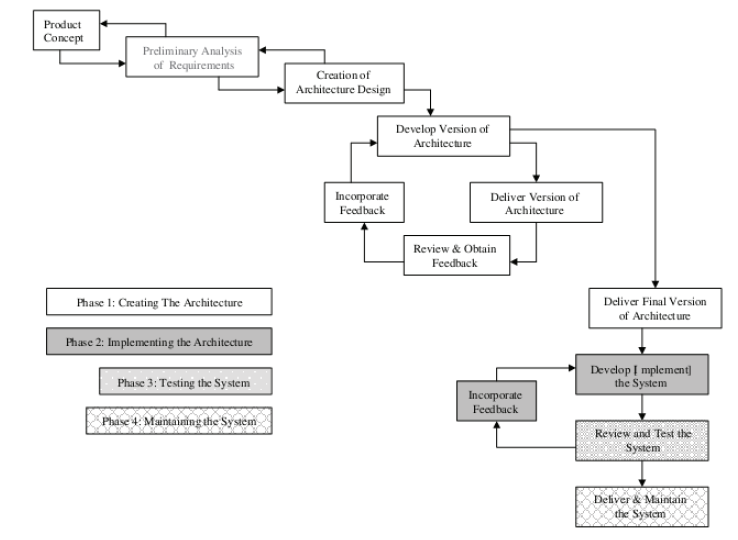
\includegraphics[width=1.0\textwidth]{Imagenes/Cap3/image001}
\end{center}
\begin{center}
\vskip -0.5cm
\caption{\small{Diseño del sistema empotrado y el modelo del ciclo de vida del desarrollo.}}
\label{fig:figura3.1}
{\small{Fuente: \cite{tammy}}}
\end{center}
\end{figure}

Como se puede ver en la Figura \ref{fig:figura3.1}, en el diseño de un sistema empotrado, según la metodología de \cite{tammy}, se pueden distinguir 4 fases: 
\begin{enumerate}
\item[-]\textbf{Fase 1. Creación de la arquitectura}, el cual es el proceso de planear el diseño del sistema empotrado.
\item[-]\textbf{Fase 2. Implementación de la arquitectura}, el cual es el proceso de desarrollar el sistema empotrado. 
\item[-]\textbf{Fase 3. Testeo del sistema}, el cual es el proceso de testear el sistema empotrado para buscar problemas y luego solucionarlos. 
\item[-]\textbf{Fase 4. Mantenimiento del sistema}, el cual es el proceso de desplegar el sistema empotrado en el mercado, y proveerlo de soporte técnico para los usuarios del dispositivo por la duración del tiempo de vida del mismo.
\end{enumerate}

\section{Fase 1. Creación de la arquitectura}
Esta fase se divide en 3 etapas:
\begin{enumerate}
\item[-]Etapa 1: Tener una base técnica sólida.
\item[-]Etapa 2: Entender el ciclo de negocio de la arquitectura.
\item[-]Etapa 3: Definir los patrones arquitectónicos y modelos de referencia.
\end{enumerate}

\subsection{Etapa 1: Tener una base técnica sólida}
Esta etapa tiene como fundamento la base cognitiva de los autores de la presente tesis y ha sido descrita tanto en el título, introducción y marco teórico.

\subsection{Etapa 2: Entender el ciclo de negocio de la arquitectura}
En la Figura \ref{fig:figura3.2} vemos que el ciclo de negocio de la arquitectura de un sistema empotrado son los diferentes tipos de influencias los que generan los requerimientos del sistema, los requerimientos a su vez generan la arquitectura, luego esta produce el sistema y el sistema resultante a su vez provee los requerimientos y capacidades devuelta a la organización para futuros diseños.
\begin{figure}[H]
\begin{center}
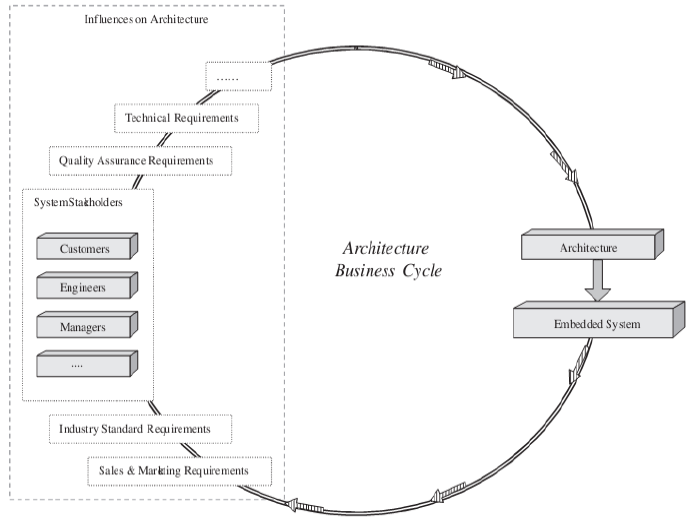
\includegraphics[width=0.5\textwidth]{Imagenes/Cap3/image002}
\end{center}
\begin{center}
\vskip -0.5cm
\caption{\small{Ciclo de negocio de la arquitectura.}}
\label{fig:figura3.2}
{\small{Fuente: \cite{tammy}}}
\end{center}
\end{figure}

Una vez entendido el ciclo de negocio de la arquitectura, se debe plasmar la información obtenida de varias influencias, que en otras palabras son los requerimientos. La presente metodología propone hacerlo mediante la tabla general de características del ciclo de negocio de la arquitectura o el uso de prototipos. Se eligió representar los requerimientos mediante la tabla general de características del ciclo de negocio de la arquitectura, ver la Tabla \ref{table:tabla3.1}.

\begin{center}
\begin{table}[H]
\centering
\caption{\small{Características generales del ciclo de negocio de la arquitectura.}}
\label{table:tabla3.1}
\vskip 0.2cm
\begin{tabular}{|p{3cm}|p{4cm}|p{6cm}|p{3cm}|}
\hline
{\small Influencia} & {\small Característica} & {\small Descripción}  \\ 
\hline 
{\small \multirow{3}{4em}{Negocios}} & {\small Costo} & {\small El sistema de seguridad para el control de acceso por medio de la voz, debe tener un costo de desarrollo menor a los S/. 500.}  \\ 
\cline{2-3}
 & {\small Objetivo de Mercado} & {\small El sistema a diseñar es del tipo de módulo reconocedor de la voz y está dirigido al control de acceso, sin embargo, puede ser usado para el control de cualquier otro objeto.}  \\ 
\cline{2-3}
 & {\small Capacidad} & {\small El sistema debe poder reconocer la voz con una tasa de acierto del 95\%. El sistema debe poder controlar los accesos para nuevos de usuarios. El sistema debe poder dar información de todos los accesos que tuvo un usuario. El sistema debe poder permitir o denegar el acceso a un usuario. El sistema debe ser capaz de trabajar en ambientes con ruido no mayores a 80 dBC.
} \\
\hline 
{\small \multirow{4}{4em}{Técnicos}} & {\small Desempeño} & {\small El sistema debe ser capaz de reconocer la voz de un locutor en un tiempo menor o igual a 5 segundos. Sin embargo, la rapidez de respuesta del sistema dependerá de la cantidad de usuarios registrados en el sistema}  \\ 
\cline{2-3}
 & {\small Amistad con Usuario} & {\small La interfaz de usuario del sistema no será muy compleja, y solo mostrará lo necesario para su manipulación.}  \\ 
\cline{2-3}
 & {\small Modificabilidad} & {\small La modificación dependerá únicamente de los desarrolladores del software}  \\ 
\cline{2-3}
 & {\small Portabilidad} & {\small El sistema podrá ser usado por cualquier dispositivo móvil Android superior a 4.4
y menor a 9.0, por lo que será portable para la mayoría de los dispositivos existentes en el mercado aproximadamente el 95\%.}  \\ 
\hline 
\end{tabular} 
\begin{center}
\vskip 0.2cm
{\small{Fuente: Elaboración propia}}
\end{center}
\end{table}
\end{center}

\subsection{Etapa 3: Definir el patrón arquitectónico y modelo de referencia}
El patrón arquitectónico a usar será el patrón arquitectónico en capas y el modelo de referencia será el modelo de referencia de sistemas empotrados, definido en \citep{tammy}. El modelo de referencia para un sistema empotrado está construido en capas y no es más que una distribución topológica de los elementos del patrón arquitectónico en capas, se define que todo sistema empotrado está formado por tres capas: de hardware, de software de sistema y de aplicación.

\begin{enumerate}
\item[a)]Capa de hardware
\par
Esta capa estará formada principalmente por un microcontrolador Arduino, el cual alojará el controlador para la activación de la cerradura eléctrica por medio del módulo relé, además este se acoplará con el módulo Ethernet Shield, lo que permitirá conectarse a un router para poder establecer así la comunicación con el dispositivo móvil.

\item[b)]Capa de software de sistema
\par
Esta capa estará formada por el controlador para la activación de la cerradura eléctrica y por el servidor para poder establecer la comunicación con la aplicación de reconocimiento de voz alojado en el dispositivo móvil.

\item[c)]Capa de software de aplicación
\par
El sistema estará formado por hardware de propósito específico, diseñado solamente para la demostración de la aplicación de reconocimiento de voz, el cual estará compuesto por 3 módulos: preprocesamiento, entrenamiento y reconocimiento de la señal de voz.

\item[d)]Modelo de referencia
\par
El modelo de referencia servirá para aproximarse al posible hardware y software que deberá contener el sistema incorporando elementos relativos. La Figura \ref{fig:figura3.3} muestra el modelo de referencia del sistema de seguridad para el control de acceso por reconocimiento de voz.
\begin{figure}[H]
\captionsetup{justification=centering}
\begin{center}
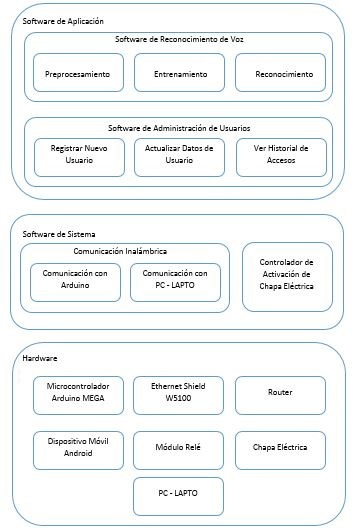
\includegraphics[width=0.43\textwidth]{Imagenes/Cap3/image003}
\end{center}
\begin{center}
\vskip -0.5cm
\caption{\small{Modelo de referencia del sistema.}}
\label{fig:figura3.3}
{\small{Fuente: Elaboración propia}}
\end{center}
\end{figure}
\end{enumerate}

\section{Fase 2. Implementación de la arquitectura}
\subsection{Desarrollo del software de aplicación}
\subsubsection{Software de reconocimiento de voz}
Primero se implementará una aplicación de escritorio en lenguaje Java, este nos permitirá evaluar y testear el algoritmo de reconocimiento de voz encontrando así las mejores funciones y los parámetros adecuados para un correcto y eficiente funcionamiento del reconocimiento de voz, para luego, finalmente ser llevado a una aplicación Android, el cual servirá como interfaz entre el usuario y el sistema. A continuación, se mostrará algunos codigos fuente de los algoritmos más importantes que usaremos para nuestro sistema de reconocimiento de voz.

\begin{enumerate}
\item[a)]Eliminación de ruido
\par
En la Figura \ref{fig:figura3.8} podemos ver la función del algoritmo NLMS definido por las Ecuaciones \eqref{eq:ecuacion10}, \eqref{eq:ecuacion11}, \eqref{eq:ecuacion12} y \eqref{eq:ecuacion13}, donde $beta/DEN$ es el factor de convergencia, $nord$ el tamaño del filtro y $a0$ el vector de pesos inicial.
\begin{figure}[H]
\captionsetup{justification=centering}
\begin{center}
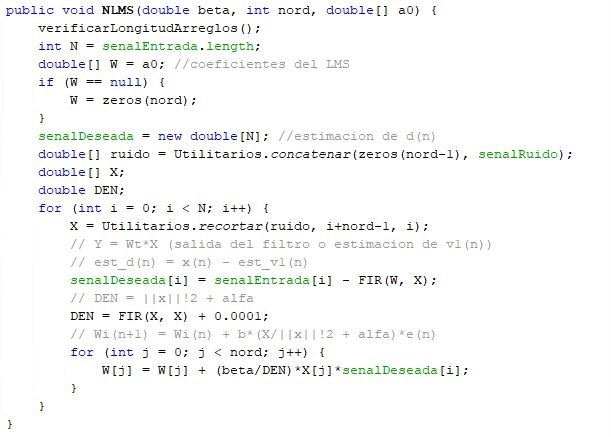
\includegraphics[width=0.6\textwidth]{Imagenes/Cap3/image008}
\end{center}
\begin{center}
\vskip -0.5cm
\caption{\small{Código fuente del algoritmo NLMS.}}
\label{fig:figura3.8}
{\small{Fuente: Elaboración propia}}
\end{center}
\end{figure}
\vskip -0.5cm
Al eliminar el ruido en la señal de voz a veces esta puede quedar con valores que sobrepasan el valor de cuantificación dado inicialmente, por lo que será necesario aplicar una normalización en la señal, esta función se muestra en la Figura \ref{fig:figura3.9} definida por las Ecuaciones \eqref{eq:ecuacion14}, \eqref{eq:ecuacion15} y \eqref{eq:ecuacion16}.
\begin{figure}[H]
\captionsetup{justification=centering}
\begin{center}
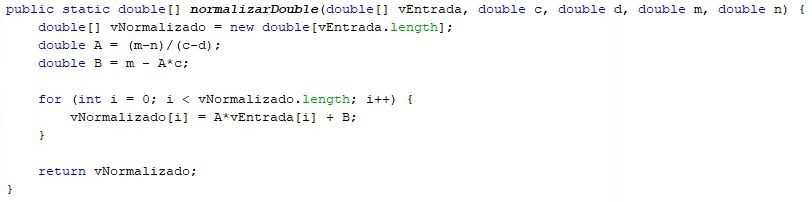
\includegraphics[width=0.8\textwidth]{Imagenes/Cap3/image009}
\end{center}
\begin{center}
\vskip -0.5cm
\caption{\small{Código fuente de la función de normalización de datos.}}
\label{fig:figura3.9}
{\small{Fuente: Elaboración propia}}
\end{center}
\end{figure}
\vskip -0.5cm
\item[b)]Filtro preénfasis
\par
En la Figura \ref{fig:figura3.10} se muestra la función para el filtro de preénfasis definida en la Ecuación \eqref{eq:ecuacion32}, donde $vEntrada$ es el vector de datos de la señal a filtrar y $alfa$ el parámetro de preénfasis.
\begin{figure}[H]
\captionsetup{justification=centering}
\begin{center}
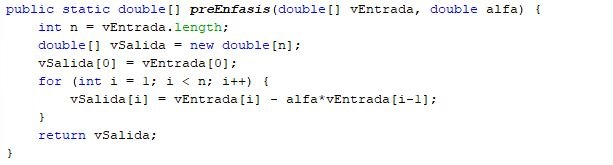
\includegraphics[width=0.7\textwidth]{Imagenes/Cap3/image010}
\end{center}
\begin{center}
\vskip -0.5cm
\caption{\small{Código fuente de la función del filtro de preénfasis.}}
\label{fig:figura3.10}
{\small{Fuente: Elaboración propia}}
\end{center}
\end{figure}
\vskip -0.5cm
\item[c)]Detección de inicio y fin de la señal de voz
\par
La Figura \ref{fig:figura3.13} muestra la función de energía de tiempo corto definida en la Ecuación \eqref{eq:ecuacion22}.
\begin{figure}[H]
\captionsetup{justification=centering}
\begin{center}
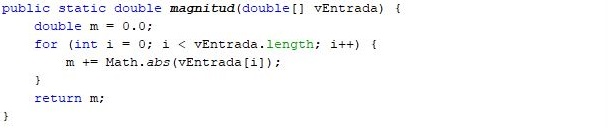
\includegraphics[width=0.7\textwidth]{Imagenes/Cap3/image013}
\end{center}
\begin{center}
\vskip -0.5cm
\caption{\small{Código fuente de la función de energía de tiempo corto.}}
\label{fig:figura3.13}
{\small{Fuente: Elaboración propia}}
\end{center}
\end{figure}
\vskip -0.5cm
En la Figura \ref{fig:figura3.14} se muestra la función de la tasa de cruce por ceros definida por las Ecuaciones \eqref{eq:ecuacion19}, \eqref{eq:ecuacion20}, \eqref{eq:ecuacion21} y \eqref{eq:ecuacion23}.
\begin{figure}[H]
\captionsetup{justification=centering}
\begin{center}
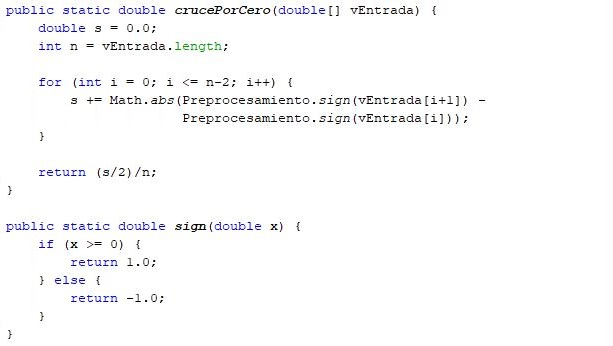
\includegraphics[width=0.75\textwidth]{Imagenes/Cap3/image014}
\end{center}
\begin{center}
\vskip -0.5cm
\caption{\small{Código fuente de la función de tasa de cruce por ceros.}}
\label{fig:figura3.14}
{\small{Fuente: Elaboración propia}}
\end{center}
\end{figure}
\vskip -0.5cm
En la Figura \ref{fig:figura3.17} se muestra el algoritmo de Rabiner y Sambur de Tipo 1, definido por las Ecuaciones \eqref{eq:ecuacion22}, \eqref{eq:ecuacion23}, \eqref{eq:ecuacion24}, \eqref{eq:ecuacion25} y \eqref{eq:ecuacion26}, teniendo como entradas a $vEntrada$ que es el vector de datos de la señal y $tamTrana$ que es la longitud de la trama con la que se hará la evaluación, retornando el punto de inicio o fin de la voz en la señal según sea el caso.

\begin{figure}[H]
\captionsetup{justification=centering}
\begin{center}
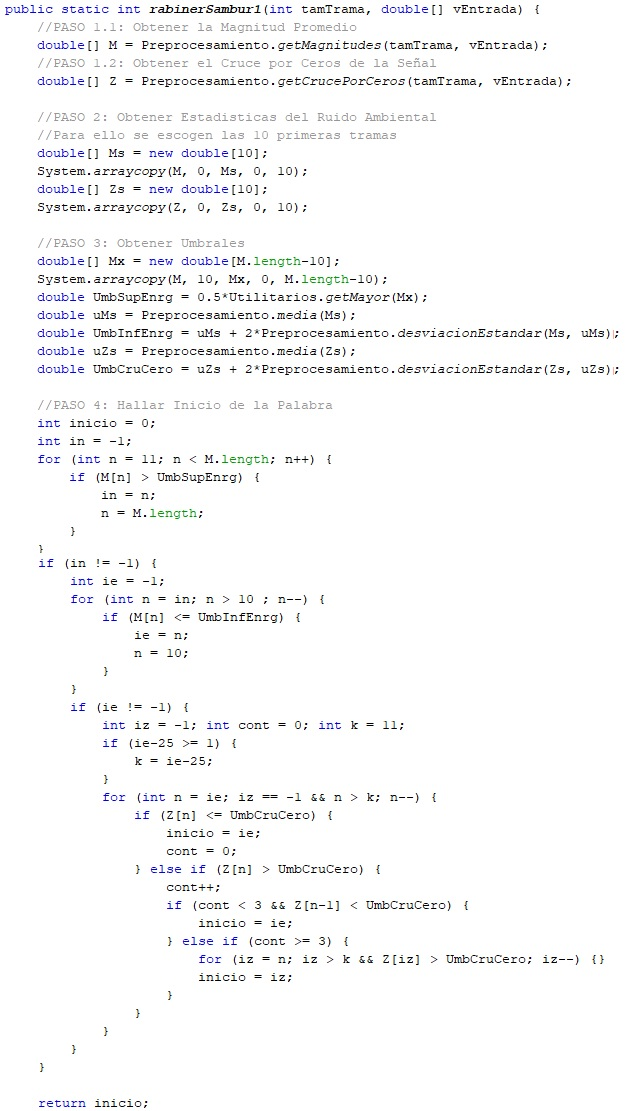
\includegraphics[width=0.65\textwidth]{Imagenes/Cap3/image017}
\end{center}
\begin{center}
\vskip -0.5cm
\caption{\small{Código fuente del algoritmo Rabiner y Sambur Tipo 1.}}
\label{fig:figura3.17}
{\small{Fuente: Elaboración propia}}
\end{center}
\end{figure}
\vskip -0.5cm
\item[d)]Segmentación
\par
En la Figura \ref{fig:figura3.19} se muestra la función para la segmentación de una señal definida por las Ecuaciones \eqref{eq:ecuacion33} y \eqref{eq:ecuacion34}, además se aplica un ponderado por una ventana.
\begin{figure}[H]
\captionsetup{justification=centering}
\begin{center}
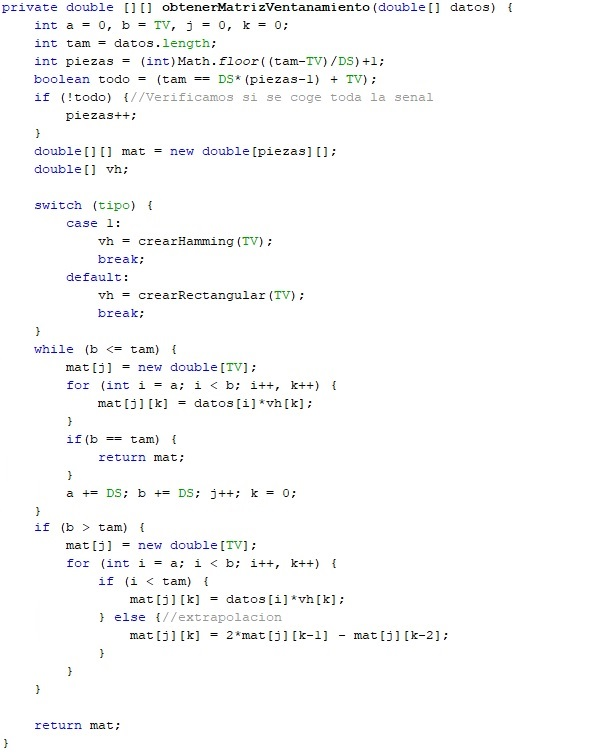
\includegraphics[width=0.65\textwidth]{Imagenes/Cap3/image019}
\end{center}
\begin{center}
\vskip -0.5cm
\caption{\small{Código fuente de la función para la segmentación de una señal.}}
\label{fig:figura3.19}
{\small{Fuente: Elaboración propia}}
\end{center}
\end{figure}
\vskip -0.5cm
\item[e)]Transformada rápida de Fourier
\par
En la Figura \ref{fig:figura3.23} se muestra la función para la transformada rápida de Fourier, definida por las Ecuación \eqref{eq:ecuacion43} y \eqref{eq:ecuacion44}, como podemos ver esta función es un método recursivo que tiene como entradas a $vEntrada$ y $N$, que son el vector de datos de la señal (rellenado con ceros) y el tamaño de este vector respectivamente.
\begin{figure}[H]
\captionsetup{justification=centering}
\begin{center}
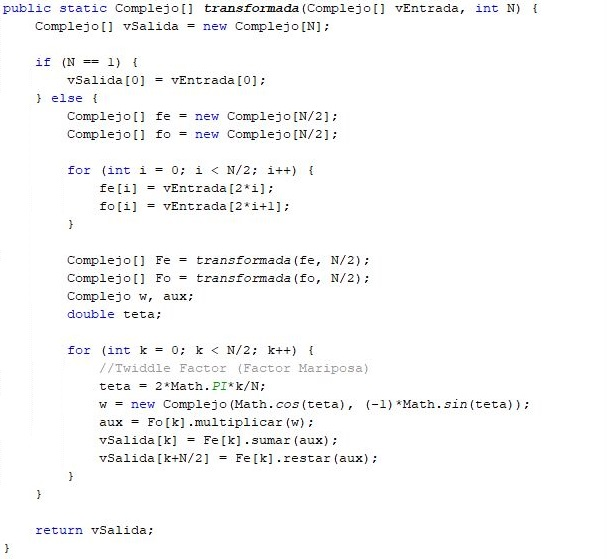
\includegraphics[width=0.7\textwidth]{Imagenes/Cap3/image023}
\end{center}
\begin{center}
\vskip -0.5cm
\caption{\small{Código fuente de la función de la transformada rápida de Fourier.}}
\label{fig:figura3.23}
{\small{Fuente: Elaboración propia}}
\end{center}
\end{figure}
\vskip -0.5cm
\item[f)]Filtrado e integración o remuestreo por bandas críticas
\par
En la Figura \ref{fig:figura3.25} se muestra la función de remuestreo por bandas críticas, definido por las Ecuaciones desde \eqref{eq:ecuacion49} hasta \eqref{eq:ecuacion57}, esta función tiene como entradas a $fmin$ y a $fmax$ que son la frecuencia mínima y máxima de la señal respectivamente.
\begin{figure}[H]
\captionsetup{justification=centering}
\begin{center}
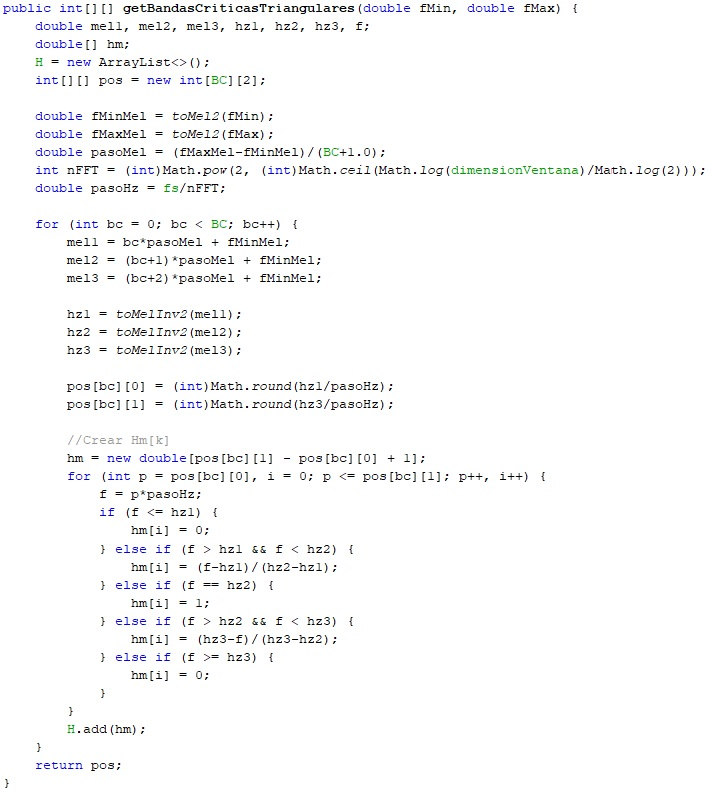
\includegraphics[width=0.72\textwidth]{Imagenes/Cap3/image025}
\end{center}
\begin{center}
\vskip -0.5cm
\caption{\small{Código fuente de la función de remuestreo por bandas críticas.}}
\label{fig:figura3.25}
{\small{Fuente: Propia}}
\end{center}
\end{figure}
\newpage
\item[g)]Obtención de los coeficientes MFCC
\par
La Figura \ref{fig:figura3.26} muestra la función para la obtención de los coeficientes MFCC, definido por las Ecuaciones \eqref{eq:ecuacion63}, \eqref{eq:ecuacion64} y \eqref{eq:ecuacion65}. Estas ecuaciones definen las etapas de compresión y la transformada discreta inversa de Fourier de la señal.
\begin{figure}[H]
\captionsetup{justification=centering}
\begin{center}
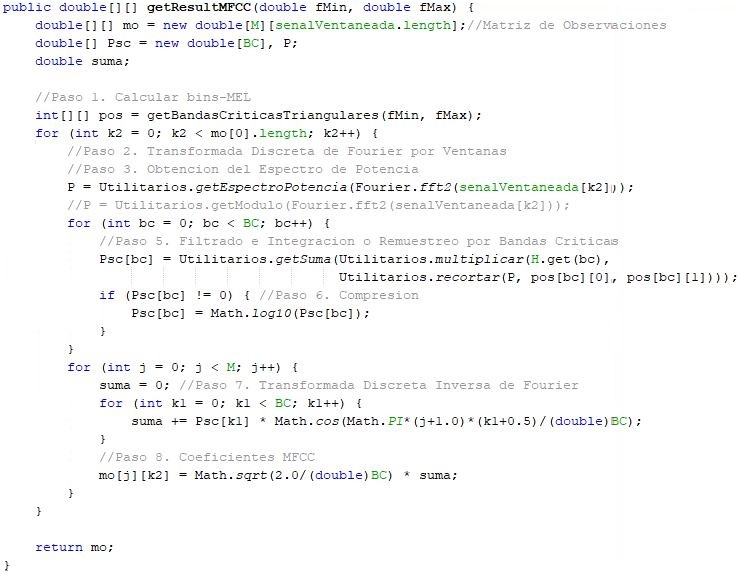
\includegraphics[width=0.85\textwidth]{Imagenes/Cap3/image026}
\end{center}
\begin{center}
\vskip -0.5cm
\caption{\small{Código fuente de la función para la obtención de coeficientes MFCC.}}
\label{fig:figura3.26}
{\small{Fuente: Elaboración propia}}
\end{center}
\end{figure}
\newpage
\item[h)]Medidas de distorsión
\par
En las Figura \ref{fig:figura3.30} se muestra las funcion de la distancia de error cuadrático medio entre dos señales de voz, definida por la Ecuación \eqref{eq:ecuacion100}.

\begin{figure}[H]
\captionsetup{justification=centering}
\begin{center}
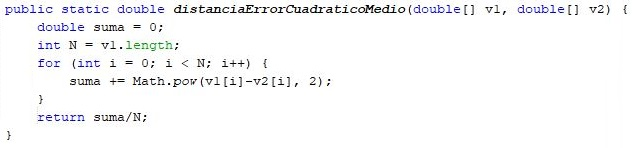
\includegraphics[width=0.7\textwidth]{Imagenes/Cap3/image030}
\end{center}
\begin{center}
\vskip -0.5cm
\caption{\small{Código fuente de la función de distancia de error cuadrático medio.}}
\label{fig:figura3.30}
{\small{Fuente: Elaboración propia}}
\end{center}
\end{figure}
\vskip -0.5cm
\item[i)]Alineamiento temporal dinámico
\par
En la Figura \ref{fig:figura3.32} se muestra la función DTW de tipo simétrico con slope constrain $P = 1/2$ sin ventana de ajuste en la comparación de patrones.
\begin{figure}[H]
\captionsetup{justification=centering}
\begin{center}
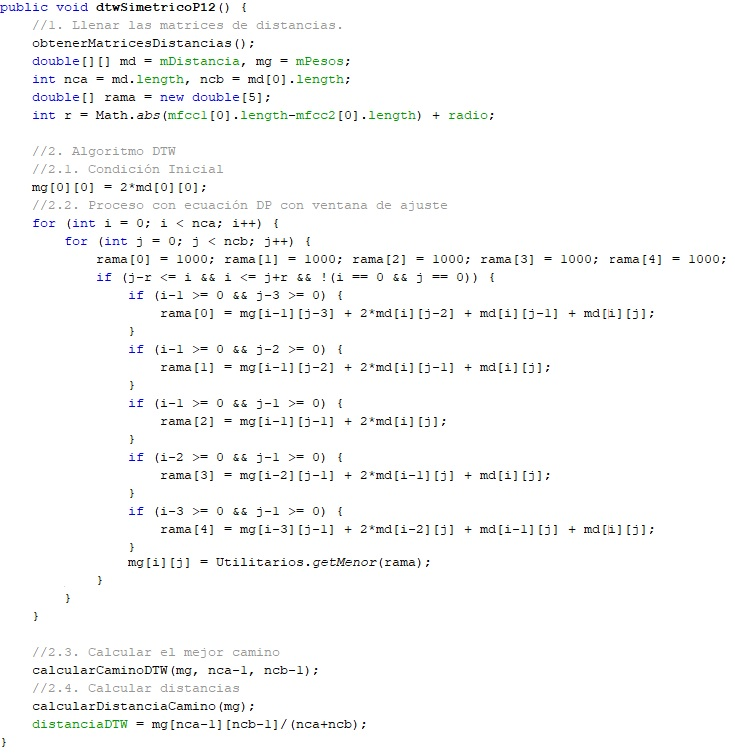
\includegraphics[width=0.79\textwidth]{Imagenes/Cap3/image032}
\end{center}
\begin{center}
\vskip -0.5cm
\caption{\small{Código fuente de la función de DTW simétrico con P = 1/2 sin ventana de ajuste.}}
\label{fig:figura3.32}
{\small{Fuente: Elaboración propia}}
\end{center}
\end{figure}

\item[j)]Construcción del patrón de referencia
\par
En la Figura \ref{fig:figura3.33} tenemos la función $indicesMinAnterior$ que nos permite hallar el punto anterior con menor peso en la matriz de comparación de patrones $mg$, esta es usada por la función $calcularCaminoDTW$, la cual permite obtener el camino con menor distancia $y_{w(n)}$, definida por la Ecuación \eqref{eq:ecuacion101}, llamada función warping o función de alineamiento.
\begin{figure}[H]
\captionsetup{justification=centering}
\begin{center}
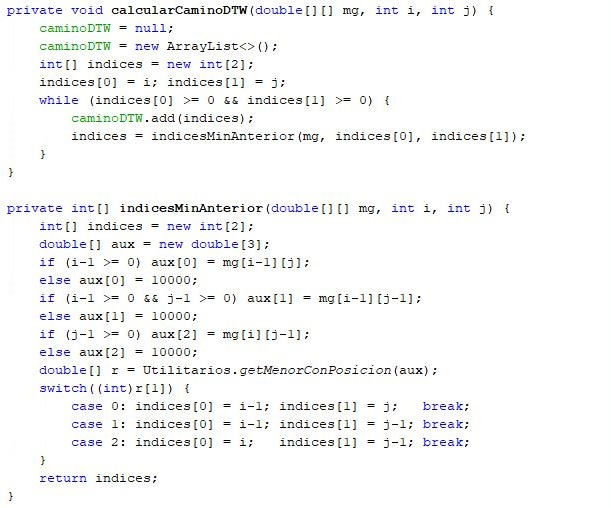
\includegraphics[width=0.7\textwidth]{Imagenes/Cap3/image033}
\end{center}
\begin{center}
\vskip -0.5cm
\caption{\small{Código fuente de la función para obtener el recorrido mínimo DTW.}}
\label{fig:figura3.33}
{\small{Fuente: Elaboración propia}}
\end{center}
\end{figure}
\vskip -0.5cm
En la Figura \ref{fig:figura3.34} se muestra la función para la construcción de los patrones de referencia, definido por la Ecuación \eqref{eq:ecuacion101}.
\begin{figure}[H]
\captionsetup{justification=centering}
\begin{center}
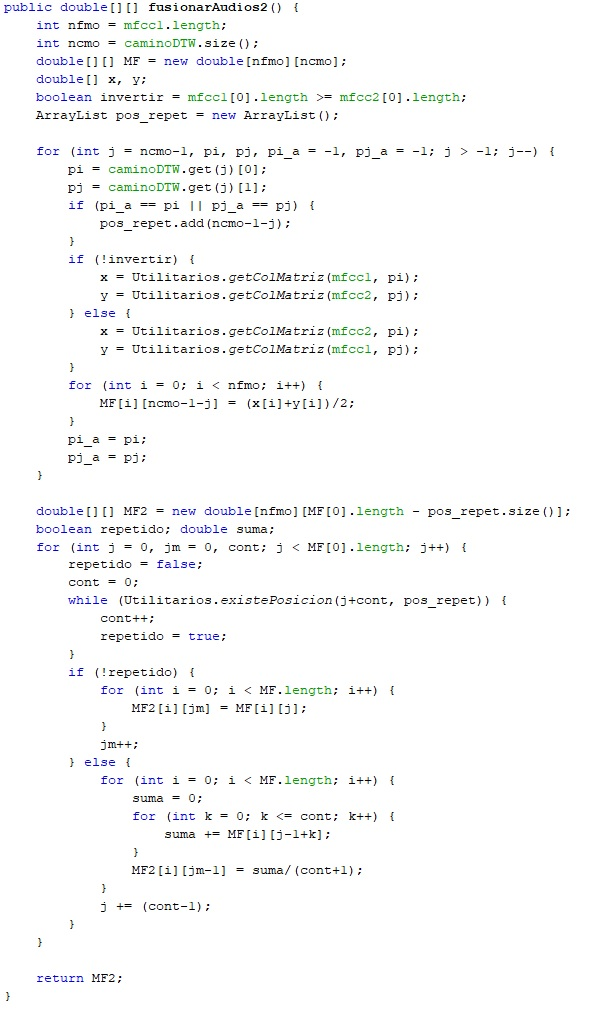
\includegraphics[width=0.7\textwidth]{Imagenes/Cap3/image034}
\end{center}
\begin{center}
\vskip -0.5cm
\caption{\small{Código fuente de la función para la construcción del patrón de referencia.}}
\label{fig:figura3.34}
{\small{Fuente: Elaboración propia}}
\end{center}
\end{figure}
\end{enumerate}

\newpage
\subsubsection{Software de administración de usuarios}
A continuación, veremos algunas de las interfaces gráficas de usuario del software de aplicación del sistema de control de acceso por reconocimiento de voz. En la Figura \ref{fig:figura3.35} podemos ver la primera interfaz que se mostrará después de haber instalado la aplicación en el dispositivo móvil Android, donde tendremos dos opciones \textit{Iniciar} y \textit{Crear Cuenta}. La primera es cuando ya se tiene un usuario del tipo \textit{Administrador}, pero sin tener aún el registro de su patrón de voz de clave de acceso, en caso de no ocurrir esto entonces se escogerá la segunda opción.
\begin{figure}[H]
\captionsetup{justification=centering}
\begin{center}
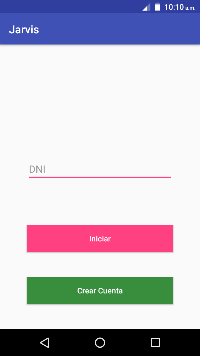
\includegraphics[width=0.25\textwidth]{Imagenes/Cap3/image035}
\end{center}
\begin{center}
\vskip -0.5cm
\caption{\small{Inicio de sesión al sistema por primera vez.}}
\label{fig:figura3.35}
{\small{Fuente: Elaboración propia}}
\end{center}
\end{figure}

Después de registrar el usuario \textit{Administrador} del sistema (esto solo se hará una sola vez), la opción \textit{Crear Cuenta} desaparecerá.

En la Figura \ref{fig:figura3.39} se muestra las opciones del menú principal del sistema que son: \textit{Comandos por Voz}, \textit{Cerrar Sesión}, \textit{Micrófono Externo}, \textit{Dispositivo Arduino}, \textit{Administrar Cuentas} y \textit{Consultar Accesos}, donde estos dos últimos solo se mostrarán para usuarios del tipo \textit{Administrador}.
\begin{figure}[H]
\captionsetup{justification=centering}
\begin{center}
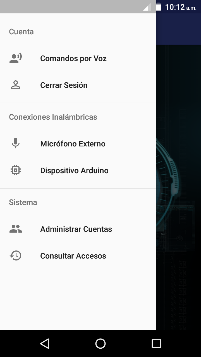
\includegraphics[width=0.25\textwidth]{Imagenes/Cap3/image039}
\end{center}
\begin{center}
\vskip -0.5cm
\caption{\small{Menú principal del sistema.}}
\label{fig:figura3.39}
{\small{Fuente: Elaboración propia}}
\end{center}
\end{figure}

En la Figura \ref{fig:figura3.40} se puede ver la interfaz para la opción del menú principal \textit{Administrar Cuentas}, donde se muestra una lista de las cuentas de los usuarios del sistema. La opción con el \textit{ícono de lupa} es para buscar usuarios, esta búsqueda puede ser por su nombre o DNI (Documento Nacional de Identidad), la opción con el \textit{ícono del mas} es para registrar un nuevo usuario al sistema, además al seleccionar un usuario de la lista podemos ver y editar sus datos.
\begin{figure}[H]
\captionsetup{justification=centering}
\begin{center}
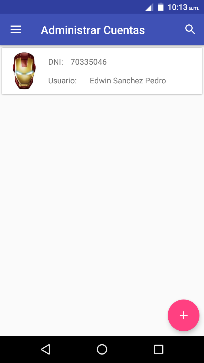
\includegraphics[width=0.25\textwidth]{Imagenes/Cap3/image040}
\end{center}
\begin{center}
\vskip -0.5cm
\caption{\small{Lista de cuentas de usuario del sistema.}}
\label{fig:figura3.40}
{\small{Fuente: Elaboración propia}}
\end{center}
\end{figure}

En la Figura \ref{fig:figura3.41} se muestra la interfaz para registrar a un nuevo usuario al sistema, donde en \textit{tipo} se especificará que tipo de acceso tendrá este usuario al sistema, si es \textit{Administrador} tendrá todos los privilegios del sistema, si es \textit{Normal} no podrá registrar ni editar los datos de los usuarios ni tampoco podrá consultar los accesos de estos al sistema y si es \textit{Sin Acceso} se le denegará el acceso al sistema.

\begin{figure}[H]
\captionsetup{justification=centering}
\begin{center}
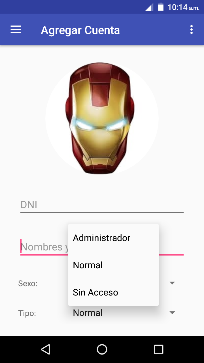
\includegraphics[width=0.25\textwidth]{Imagenes/Cap3/image041}
\end{center}
\begin{center}
\vskip -0.5cm
\caption{\small{Registrar un nuevo usuario al sistema.}}
\label{fig:figura3.41}
{\small{Fuente: Elaboración propia}}
\end{center}
\end{figure}

En la Figura \ref{fig:figura3.42} se muestra el menú con las opciones \textit{Guardar}, \textit{Patrón de Voz} y \textit{Comando de Voz}. El primero es para guardar el registro o el editado de los datos de un usuario. El segundo es para poder asignar un patrón de voz clave al usuario que le permitirá acceder al sistema. Y la última opción es para asignar los comandos de voz que realizará el sistema por parte del usuario.
\begin{figure}[H]
\captionsetup{justification=centering}
\begin{center}
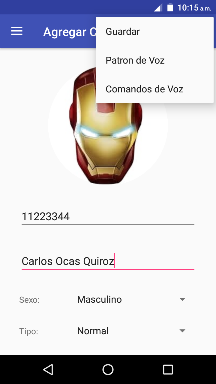
\includegraphics[width=0.25\textwidth]{Imagenes/Cap3/image042}
\end{center}
\begin{center}
\vskip -0.5cm
\caption{\small{Menú de opciones para la administración de usuarios del sistema.}}
\label{fig:figura3.42}
{\small{Fuente: Elaboración propia}}
\end{center}
\end{figure}

En la Figura \ref{fig:figura3.43} se muestra la lista de audios de los patrones de voz que conforman la clave de acceso de un usuario, esta interfaz se muestra a través de la opción \textit{Patrones de Voz} del menú de opciones que se vió en la Figura \ref{fig:figura3.42}.
\begin{figure}[H]
\captionsetup{justification=centering}
\begin{center}
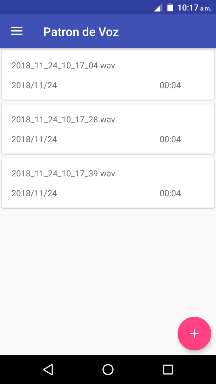
\includegraphics[width=0.25\textwidth]{Imagenes/Cap3/image043}
\end{center}
\begin{center}
\vskip -0.5cm
\caption{\small{Lista de audios del patrón clave de usuario para el acceso al sistema.}}
\label{fig:figura3.43}
{\small{Fuente: Elaboración propia}}
\end{center}
\end{figure}

En la Figura \ref{fig:figura3.44} se muestra la interfaz para la grabación de un nuevo audio, a través de la opción con \textit{ícono de mas} que se vió en la interfaz anterior en la Figura \ref{fig:figura3.43}. Como podemos ver en esta interfaz al inicio se muestran tres opciones, la primera es para iniciar la grabación, la segunda es para reproducir la grabación y la tercera es para regresar a la lista de audios.
\begin{figure}[H]
\captionsetup{justification=centering}
\begin{center}
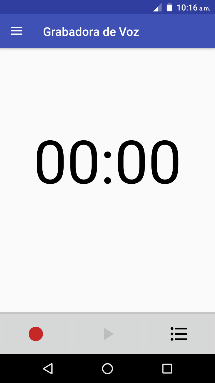
\includegraphics[width=0.25\textwidth]{Imagenes/Cap3/image044}
\end{center}
\begin{center}
\vskip -0.5cm
\caption{\small{Grabación de un nuevo audio en el sistema.}}
\label{fig:figura3.44}
{\small{Fuente: Elaboración propia}}
\end{center}
\end{figure}

Una vez terminada la grabación se mostrarán las opciones de \textit{cancelar} y \textit{aceptar} el almacenamiento del audio en la base datos, \textit{grabar} un nuevo audio, \textit{reproducir} el audio grabado, y por ultimo ir a la \textit{lista de audios}, ver la Figura \ref{fig:figura3.45}.
\begin{figure}[H]
\captionsetup{justification=centering}
\begin{center}
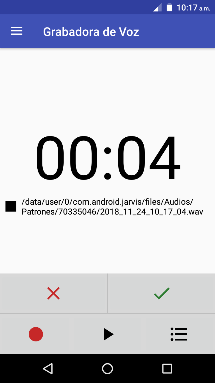
\includegraphics[width=0.25\textwidth]{Imagenes/Cap3/image045}
\end{center}
\begin{center}
\vskip -0.5cm
\caption{\small{Opciones despúes de grabar un audio en el sistema.}}
\label{fig:figura3.45}
{\small{Fuente: Elaboración propia}}
\end{center}
\end{figure}

También, podemos eliminar audios del sistema, para ello mantenemos presionado por un tiempo el audio a eliminar y así la vista cambiará a modo eliminación, permitiendo seleccionar uno a más audios a eliminar, al seleccionar la opción con \textit{ícono de tacho} se eliminarán todos los audios seleccionados de la base datos, ver la Figura \ref{fig:figura3.46}.
\begin{figure}[H]
\captionsetup{justification=centering}
\begin{center}
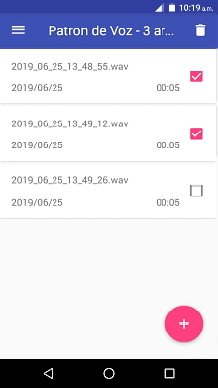
\includegraphics[width=0.25\textwidth]{Imagenes/Cap3/image046}
\end{center}
\begin{center}
\vskip -0.5cm
\caption{\small{Eliminar audios de un usuario del sistema.}}
\label{fig:figura3.46}
{\small{Fuente: Elaboración propia}}
\end{center}
\end{figure}

En la Figura \ref{fig:figura3.47} podemos ver la lista de los accesos de los usuarios del sistema, esta se mostrará a través de la opción \textit{Consultar Accesos} del menú principal del sistema mostrado en la Figura \ref{fig:figura3.39}. En esta interfaz se puede realizar búsquedas por DNI del usuario o por fecha de acceso al sistema, a través de la opción con \textit{ícono de lupa}.
\begin{figure}[H]
\captionsetup{justification=centering}
\begin{center}
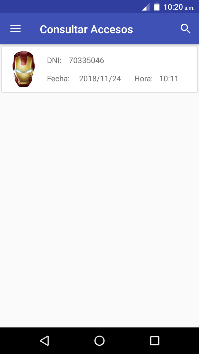
\includegraphics[width=0.25\textwidth]{Imagenes/Cap3/image047}
\end{center}
\begin{center}
\vskip -0.5cm
\caption{\small{Lista de los accesos de los usuarios en el sistema.}}
\label{fig:figura3.47}
{\small{Fuente: Elaboración propia}}
\end{center}
\end{figure}

En la Figura \ref{fig:figura3.48} podemos observar la interfaz que nos permitirá realizar el reconocimiento del usuario para su acceso al sistema, así como los comandos de voz. A través de la opción con \textit{ícono de cámara}, nos permitirá cambiar la foto de la cuenta que ha iniciado sesíon, para ello se abrirá la cámara del dispositivo para poder tomar la foto.
\begin{figure}[H]
\captionsetup{justification=centering}
\begin{center}
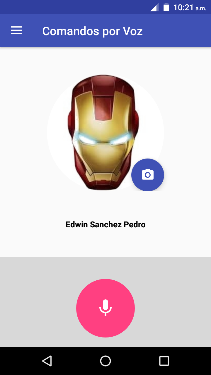
\includegraphics[width=0.25\textwidth]{Imagenes/Cap3/image048}
\end{center}
\begin{center}
\vskip -0.5cm
\caption{\small{Interfaz para el reconocimiento del usuario y comandos por voz.}}
\label{fig:figura3.48}
{\small{Fuente: Elaboración propia}}
\end{center}
\end{figure}

En la Figura \ref{fig:figura3.50} se muestra la grabación de un comando de voz para su reconocimiento por parte del sistema, a través de la opción con \textit{ícono de micrófono} (el tiempo máximo de grabación es de un minuto), una vez terminada la grabación esta puede ser cancelada o enviada para su procesamiento y reconocimiento del comando de voz.
\begin{figure}[H]
\captionsetup{justification=centering}
\begin{center}
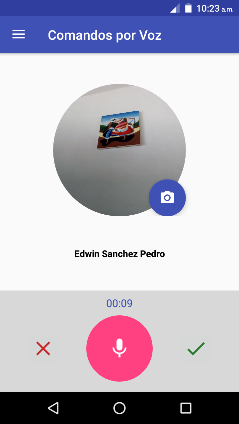
\includegraphics[width=0.25\textwidth]{Imagenes/Cap3/image050}
\end{center}
\begin{center}
\vskip -0.5cm
\caption{\small{Cancelar o enviar el comando de voz para su reconocimiento.}}
\label{fig:figura3.50}
{\small{Fuente: Elaboración propia}}
\end{center}
\end{figure}

En el reconocimiento pueden darse los resultados de \textit{usuario reconocido, usuario no reconocido, usted no es el usuario, comando reconocido o comando no reconocido.} En la Figura \ref{fig:figura3.51} se muestra el reconocimiento del comando de voz \textit{encender}. Para esta aplicación solo se reconocerán los comandos \textit{encender}, \textit{apagar} y \textit{jarvis}.
\begin{figure}[H]
\captionsetup{justification=centering}
\begin{center}
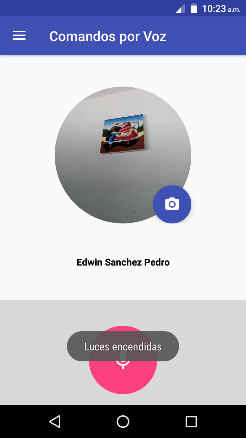
\includegraphics[width=0.25\textwidth]{Imagenes/Cap3/image051}
\end{center}
\begin{center}
\vskip -0.5cm
\caption{\small{Reconocimiento del comando de voz encender.}}
\label{fig:figura3.51}
{\small{Fuente: Elaboración propia}}
\end{center}
\end{figure}

Después de dar en la opción \textit{Cerrar Sesión} del menú principal de la Figura \ref{fig:figura3.39}, nos llevará a la pantalla principal. En la Figura \ref{fig:figura3.53} se muestra el menú principal antes de iniciar sesión al sistema con una cuenta de usuario.

\begin{figure}[H]
\captionsetup{justification=centering}
\begin{center}
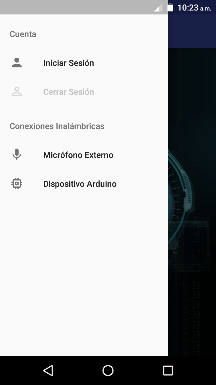
\includegraphics[width=0.25\textwidth]{Imagenes/Cap3/image053}
\end{center}
\begin{center}
\vskip -0.5cm
\caption{\small{Menú de opciones antes de iniciar sesión en el sistema.}}
\label{fig:figura3.53}
{\small{Fuente: Elaboración propia}}
\end{center}
\end{figure}

Para iniciar sesión debemos ir a la opción \textit{Iniciar Sesión} del menú principal, ver la Figura \ref{fig:figura3.53}, donde se nos mostrará la interfaz para poder hacer la grabación del patrón clave de voz a reconocer, esta interfaz es la misma que para grabar comandos que se vió en la Figura \ref{fig:figura3.50}. Si el patrón clave de acceso es incorrecto, o si el usuario todavía no se ha registrado o si un usuario quiere hacerse pasar por otro usuario se mostrará un mensaje de error, tal como se ve en la Figura \ref{fig:figura3.54}.
\begin{figure}[H]
\captionsetup{justification=centering}
\begin{center}
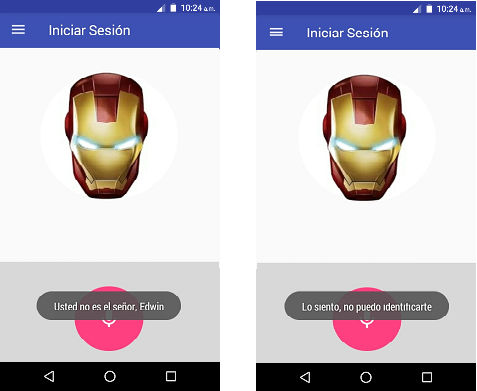
\includegraphics[width=0.55\textwidth]{Imagenes/Cap3/image054}
\end{center}
\begin{center}
\vskip -0.5cm
\caption{\small{Respuestas después de tratar de acceder al sistema.}}
\label{fig:figura3.54}
{\small{Fuente: Elaboración propia}}
\end{center}
\end{figure}

En la Figura \ref{fig:figura3.60} se muestra un mensaje de error al momento de establecer la comunicación con el Arduino para el control del hardware del sistema, a través de la opción \textit{Dispositivo Arduino} del menú principal, esto se debe a que el Arduino se encuentra apagado. Por otro lado, en la Figura \ref{fig:figura3.61} se muestra un mensaje de una conexión correcta con el Arduino, permitiendo así el control del hardware del sistema.
\begin{figure}[H]
\captionsetup{justification=centering}
\begin{center}
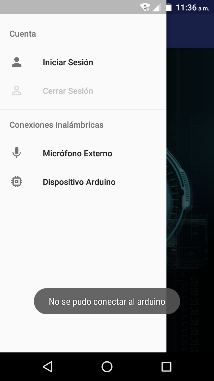
\includegraphics[width=0.25\textwidth]{Imagenes/Cap3/image060}
\end{center}
\begin{center}
\vskip -0.5cm
\caption{\small{Error en la conexión con arduino.}}
\label{fig:figura3.60}
{\small{Fuente: Elaboración propia}}
\end{center}
\end{figure}

\begin{figure}[H]
\captionsetup{justification=centering}
\begin{center}
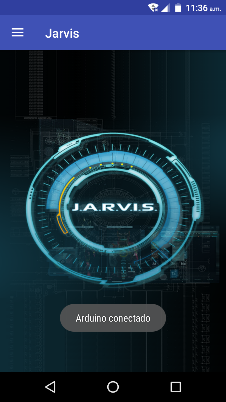
\includegraphics[width=0.25\textwidth]{Imagenes/Cap3/image061}
\end{center}
\begin{center}
\vskip -0.5cm
\caption{\small{Conexión establecida con arduino.}}
\label{fig:figura3.61}
{\small{Fuente: Elaboración propia}}
\end{center}
\end{figure}

\newpage
\subsection{Desarrollo del software del sistema}
Esta etapa consiste en construir los algoritmos utilizados para establecer la comunicación entre el software de aplicación y el hardware del sistema, esta está conformada por tres módulos \textit{Controlador de Activación de la Cerradura Eléctrica}, \textit{Comunicación con el Arduino} y \textit{Comunicación con el Computador}, ver la Figura \ref{fig:figura3.3}.
\vskip 0.5cm
El módulo \textit{Comunicación con Computador} consiste en implementar un algoritmo tanto en el dispositivo móvil como en el computador, para establecer la comunicación entre ellos para el uso del micrófono para la grabación del ruido del ambiente. A continuación, mostraremos los códigos fuentes de la implementación de los otros módulos restantes.
\vskip 0.5cm
En la Figura se muestra el código fuente que se implementará en el Arduino para establecer la comunicación con el dispositivo móvil, para poder desde este manipular el hardware del sistema, para nuestro caso solo se ralizarán las acciones de \textit{abrir}, \textit{cerrar}, \textit{encender} y \textit{apagar}.

\begin{figure}[H]
\captionsetup{justification=centering}
\begin{center}
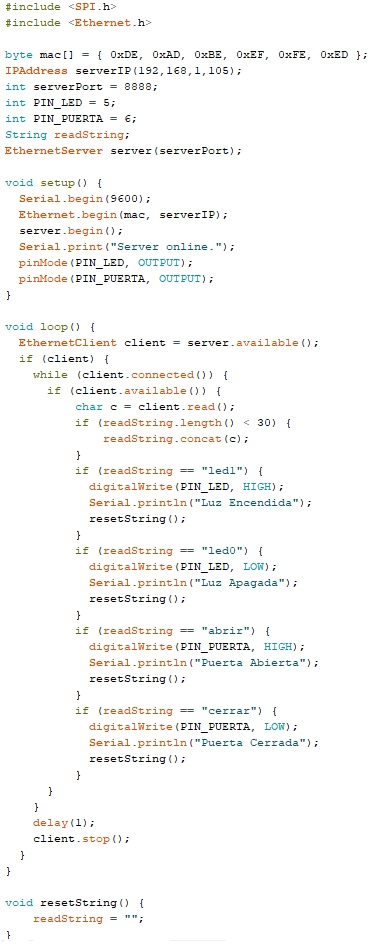
\includegraphics[width=0.4\textwidth]{Imagenes/Cap3/image062}
\end{center}
\begin{center}
\vskip -0.5cm
\caption{\small{Código fuente para establecer la comunicación con el dispositivo móvil en arduino.}}
\label{fig:figura3.62}
{\small{Fuente: Elaboración propia}}
\end{center}
\end{figure}

En la Figura \ref{fig:figura3.63} se muestra el código fuente que se implementará en la aplicación del dispositivo móvil para la comunicación con el arduino para la manipulación del hardware del sistema.
\begin{figure}[H]
\captionsetup{justification=centering}
\begin{center}
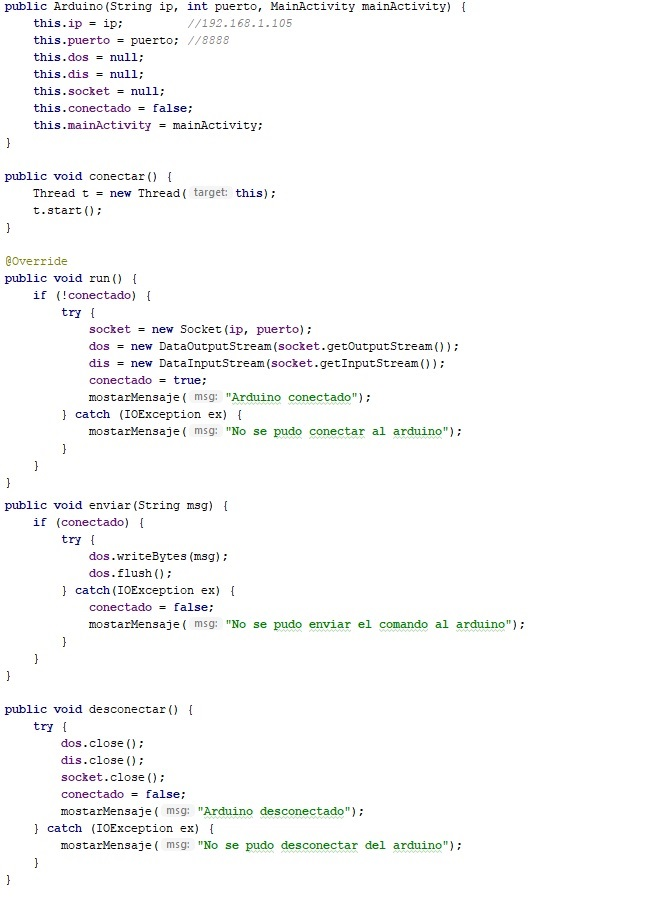
\includegraphics[width=0.65\textwidth]{Imagenes/Cap3/image063}
\end{center}
\begin{center}
\vskip -0.5cm
\caption{\small{Código fuente para establecer la comunicación con el arduino en android.}}
\label{fig:figura3.63}
{\small{Fuente: Elaboración propia}}
\end{center}
\end{figure}

\subsection{Construcción del hardware}
\subsubsection{Instrumentos}
\begin{enumerate}
\item[-]Un dispositivo móvil con Android 8.0, memoria RAM 3GB y CPU 4x1.4GHz.
\item[-]Un computador con Windows 10, memoria RAM 8GB y CPU Intel Core i5 2x2.60GHz.
\item[-]Un módem router pasarela con tecnología 802.11 b,g,n.
\item[-]Un Arduino Mega 2560 R3.
\item[-]Un módulo Ethernet Shield W5100 compatible con Arduino Mega.
\item[-]Un módulo relé 4 Songle 10A 250VAC.
\item[-]Un transformador DC 9-12V 1A.
\item[-]Un transformador DC 5V 500mA.
\item[-]Un transformador DC 12V 1A.
\item[-]Una cerradura eléctrica YALE.
\item[-]Un foco ahorrador de 200V y 65W.
\end{enumerate}
\subsubsection{Diseño del hardware del sistema}
En la Figura \ref{fig:figura3.69} se muestra el diseño del hardware para nuestro sistema de seguridad por reconocimiento de voz, en dicho diagrama se indica la conexión e integración de cada componente que conforman el hardware del sistema. A continuación, explicaremos el rol que cumple cada componente en el funcionamiento del sistema.
\vskip 0.5cm
El arduino mega, este microcontrolador almacena el código fuente que nos permitirá controlar la activación o desactivación de la cerradura eléctrica y el foco, a través de un dispositivo móvil android, para ello se nececita establecer una comunicación inalámbrica con este, es por eso que se utiliza el componente ethernet shield, el cuál nos permite conectar el arduino mega a una red por medio de un cable UTP con entradas de tipo RJ45, y este es conectado a un router o móden.
\vskip 0.5cm
En cuanto al módulo relé, este componente su función es transformar el voltaje de la corriente eléctrica de 0V a 5V proveniente del arduino mega a 220V, que es usada para la activación del foco y de la cerradura eléctrica, pero para este último se requiere para su funcionamiento 12V, por lo que se usa un tranformador reductor de potencial.
\begin{figure}[H]
\captionsetup{justification=centering}
\begin{center}
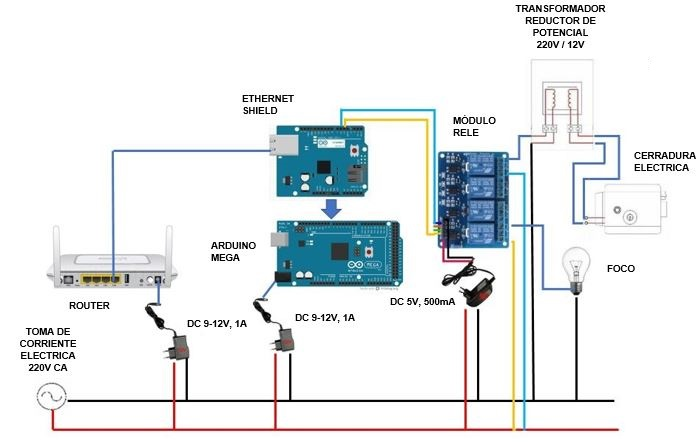
\includegraphics[width=0.62\textwidth]{Imagenes/Cap3/image069}
\end{center}
\begin{center}
\vskip -0.5cm
\caption{\small{Diseño del hardware del sistema de reconocimiento de voz.}}
\label{fig:figura3.69}
{\small{Fuente: Elaboración propia}}
\end{center}
\end{figure}

\subsubsection{Implementación del hardware del sistema}
En la Figura \ref{fig:figura3.70} se muestra la implementación del hardware de nuestro sistema de seguridad por reconocimiento de voz.
\begin{figure}[H]
\captionsetup{justification=centering}
\begin{center}
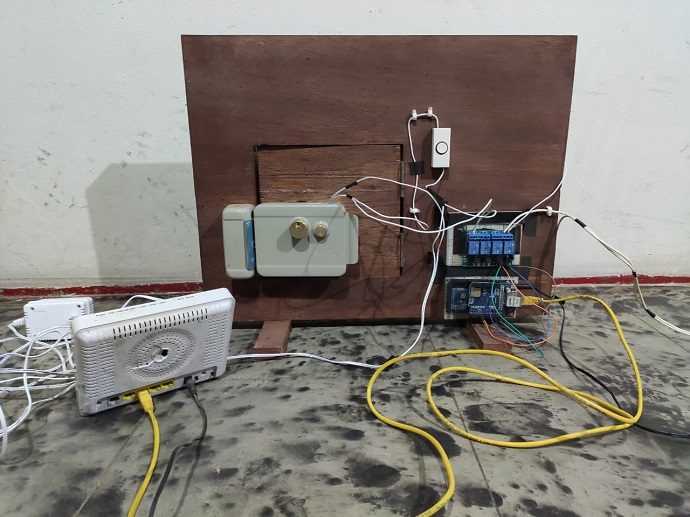
\includegraphics[width=0.42\textwidth]{Imagenes/Cap3/image070}
\end{center}
\begin{center}
\vskip -0.5cm
\caption{\small{Implementación del hardware del sistema de reconocimiento de voz.}}
\label{fig:figura3.70}
{\small{Fuente: Elaboración propia}}
\end{center}
\end{figure}
\vskip -0.5cm
\newpage
\section{Fase 3. Testeo del sistema}
En esta etapa del desarrollo utilizaremos a 5 personas del sexo masculino con edades entre 20 y 22 años, donde cada uno de ellos dirá los números del 1 al 10, repitiendo este proceso 5 veces, el entorno de grabación será en un ambiente controlado (sin ruido).
\vskip 0.5cm
Una vez recolectado las 250 grabaciones, donde cada persona pronunció cada número 5 veces, 3 de ellos los utilizaremos para la etapa de entrenamiento (150 audios) y los 2 restantes para el testeo del sistema (100 audios). Las grabaciones se realizaron con una frecuencia de muestro de 16000 Hz, canal mono, 16 bits de cuantificación y la codificación Little-Endian.
\vskip 0.5cm
A continuación, veremos los resultados obtenidos de las evaluaciones para cada configuración del algoritmo de reconocimiento de voz, mostrando el número de reconocimientos incorrectos obtenidos, donde \textit{min} es el número mínimo de errores (desaciertos en el reconocimiento) obtenidos para una configuración (algoritmo con determinados valores en los parámetros), \textit{prom} es el valor promedio de los errores obtenidos para una configuración, y finalmente \textit{error} es el promedio de los valores \textit{prom} obtenidos.

% ------------------- TABLAS -----------------------%
\subsection{Hallar BC y M}
En este primer testeo hallaremos $BC$ y $M$, parámetros del algoritmo MFCC empleado para obtener el patrón característico de una señal de voz, teniendo la siguiente configuración del algoritmo:\\
- Filtro Preénfasis \\
\hspace*{1cm} $\alpha$ = Desde 0.80 hasta 0.97 \\
- Segmentación por Hamming\\
\hspace*{1cm} V = 30 ; \qquad S = 12, 14, 15 y 16\\
- MFCC\\
\hspace*{1cm} BC = 13, 15, 18, 20, 22 y 24 ; \qquad M = 13, 15, 26 y 39\\
- DTW\\
\hspace*{1cm} P = 1 Simétrico ; \qquad R = 40 ; \qquad D = Euclidiana Cuadrática

\begin{center}
\begin{table}[H]
\centering
\caption{\small{Resultados del testeo del sistema para BC = 13, 16 y 18 con M = 13.}}
\label{table:tabla3.2}
\vskip 0.2cm
\scalebox{0.54}{
\begin{tabular}{|c|c|c|c|c|c|c|c|c|c|c|c|c|c|}
\hline 
{} & 
\multicolumn{4}{c|}{BC=13 M=13 V=30 P=S1 R=40} & 
\multicolumn{4}{c|}{BC=16 M=13 V=30 P=S1 R=40} & 
\multicolumn{4}{c|}{BC=18 M=13 V=30 P=S1 R=40}  \\ 
\hline 
$\alpha$ & 
S=16(2.5m) & S=15(3.1m) & S=14(4.1m) & S=12(5m)& 
S=16(3.4m) & S=15(4.1m) & S=14(4.2m) & S=12(5m)& 
S=16(3.4m) & S=15(4m) & S=14(4.2m) & S=12(5m) \\ 
\hline 
0.8 & 
4 & 4 & 3 & 4 & 7 & 5 & 8 & 8 & 6 & 5 & 8 & 6 \\
\hline 
0.81 & 
4 & 4 & 3 & 4 & 6 & 6 & 7 & 9 & 5 & 6 & 10 & 6 \\
\hline 
0.82 & 
4 & 4 & 3 & 4 & 7 & 3 & 7 & 10 & 7 & 7 & 10 & 6 \\
\hline 
0.83 & 
4 & 4 & 3 & 4 & 7 & 4 & 6 & 10 & 8 & 7 & 10 & 6 \\
\hline 
0.84 & 
4 & 4 & 3 & 4 & 7 & 4 & 4 & 9 & 8 & 7 & 10 & 9 \\
\hline 
0.85 & 
4 & 4 & 3 & 4 & 8 & 6 & 5 & 7 & 8 & 8 & 10 & 8 \\ 
\hline 
0.86 & 
4 & 4 & 3 & 4 & 6 & 4 & 5 & 6 & 7 & 6 & 9 & 7 \\
\hline 
0.87 & 
4 & 4 & 3 & 4 & 7 & 5 & 6 & 6 & 7 & 5 & 7 & 8 \\
\hline 
0.88 & 
4 & 4 & 3 & 4 & 5 & 6 & 3 & 6 & 7 & 3 & 5 & 7 \\
\hline 
0.89 & 
4 & 4 & 3 & 4 & 5 & 5 & 5 & 8 & 6 & 5 & 5 & 7 \\
\hline 
0.9 & 
4 & 4 & 3 & 4 & 5 & 5 & 6 & 8 & 6 & 4 & 4 & 6 \\
\hline 
0.91 & 
4 & 4 & 3 & 4 & 4 & 6 & 6 & 6 & 6 & 3 & 5 & 6 \\
\hline 
0.92 & 
4 & 4 & 3 & 4 & 7 & 6 & 5 & 5 & 8 & 4 & 3 & 8 \\
\hline 
0.93 & 
4 & 4 & 3 & 4 & 5 & 6 & 7 & 5 & 7 & 4 & 5 & 7 \\
\hline 
0.94 & 
4 & 4 & 3 & 4 & 5 & 5 & 5 & 5 & 8 & 3 & 6 & 8 \\
\hline 
0.95 & 
4 & 4 & 3 & 4 & 5 & 4 & 6 & 5 & 8 & 5 & 7 & 6 \\
\hline 
0.96 & 
4 & 4 & 3 & 3 & 8 & 4 & 7 & 7 & 7 & 5 & 4 & 4 \\
\hline 
0.97 & 
4 & 4 & 3 & 3 & 6 & 6 & 5 & 6 & 9 & 5 & 4 & 7 \\
\hline 
min & 
4 & 4 & 3 & 3 & 4 & 3 & 3 & 5 & 5 & 3 & 3 & 4 \\
\hline 
prom & 
4 & 4 & 3 & 3.8888889 & 6.111111 & 5 & 5.722222 & 7 & 7.111111 & 5.111111 & 6.777778 & 6.777778 \\
\hline 
error & 
\multicolumn{4}{c|}{3.722222222} & 
\multicolumn{4}{c|}{5.958333333} & 
\multicolumn{4}{c|}{6.444444444}\\ 
\hline 
\end{tabular} 
}
\begin{center}
\vskip 0.2cm
{\small{Fuente: Elaboración propia}}
\end{center}
\end{table}
\end{center}

\vskip -0.5cm

\begin{center}
\begin{table}[H]
\centering
\caption{\small{Resultados del testeo del sistema para BC = 20, 22 y 24 con M = 13.}}
\label{table:tabla3.3}
\vskip 0.2cm
\scalebox{0.54}{
\begin{tabular}{|c|c|c|c|c|c|c|c|c|c|c|c|c|c|}
\hline 
{} & 
\multicolumn{4}{c|}{BC=20 M=13 V=30 P=S1 R=40} & 
\multicolumn{4}{c|}{BC=22 M=13 V=30 P=S1 R=40} & 
\multicolumn{4}{c|}{BC=24 M=13 V=30 P=S1 R=40}  \\ 
\hline 
$\alpha$ & 
S=16(3.5m) & S=15(4m) & S=14(4.2m) & S=12(5m)& 
S=16(3.5m) & S=15(4m) & S=14(4.2m) & S=12(5m)& 
S=16(3.5m) & S=15(4m) & S=14(4.2m) & S=12(5m) \\ 
\hline 
0.8 & 
5 & 7 & 6 & 6 & 4 & 4 & 3 & 3 & 5 & 4 & 3 & 3 \\
\hline 
0.81 & 
5 & 7 & 7 & 6 & 4 & 4 & 3 & 3 & 5 & 4 & 3 & 3 \\
\hline 
0.82 & 
5 & 7 & 8 & 7 & 4 & 4 & 3 & 3 & 5 & 4 & 3 & 3 \\
\hline 
0.83 & 
7 & 6 & 5 & 7 & 4 & 4 & 3 & 3 & 5 & 4 & 3 & 3 \\
\hline 
0.84 & 
6 & 7 & 7 & 7 & 4 & 4 & 3 & 3 & 5 & 4 & 3 & 3 \\
\hline 
0.85 & 
6 & 6 & 8 & 7 & 4 & 4 & 3 & 3 & 5 & 4 & 3 & 3 \\
\hline 
0.86 & 
6 & 6 & 7 & 7 & 4 & 4 & 3 & 3 & 5 & 4 & 3 & 3 \\
\hline 
0.87 & 
5 & 6 & 7 & 6 & 4 & 4 & 3 & 3 & 5 & 4 & 3 & 3 \\
\hline 
0.88 & 
6 & 7 & 6 & 6 & 4 & 4 & 3 & 3 & 5 & 4 & 3 & 3 \\
\hline 
0.89 & 
6 & 7 & 8 & 8 & 4 & 4 & 3 & 3 & 5 & 4 & 3 & 3 \\
\hline 
0.9 & 
8 & 6 & 5 & 6 & 4 & 4 & 3 & 3 & 5 & 4 & 3 & 3 \\
\hline 
0.91 & 
8 & 6 & 5 & 6 & 4 & 4 & 3 & 3 & 5 & 4 & 3 & 3 \\
\hline 
0.92 & 
7 & 4 & 4 & 5 & 4 & 4 & 3 & 3 & 5 & 4 & 3 & 3 \\
\hline 
0.93 & 
6 & 5 & 6 & 6 & 4 & 4 & 3 & 3 & 5 & 4 & 3 & 3 \\
\hline 
0.94 & 
7 & 6 & 5 & 6 & 4 & 4 & 3 & 3 & 5 & 4 & 3 & 3 \\
\hline 
0.95 & 
7 & 5 & 6 & 5 & 4 & 4 & 3 & 3 & 4 & 4 & 3 & 3 \\
\hline 
0.96 & 
5 & 4 & 6 & 5 & 4 & 4 & 3 & 3 & 4 & 4 & 3 & 3 \\
\hline 
0.97 & 
3 & 4 & 5 & 6 & 4 & 4 & 3 & 3 & 4 & 4 & 3 & 3 \\
\hline 
min & 
3 & 4 & 4 & 2 & 4 & 4 & 3 & 3 & 4 & 4 & 3 & 3 \\
\hline 
prom & 
6 & 5.888889 & 6.166667 & 6.222222 & 4 & 4 & 3 & 3 & 4.833333 & 4 & 3 & 3 \\
\hline 
error & 
\multicolumn{4}{c|}{6.069444444} & 
\multicolumn{4}{c|}{3.5} & 
\multicolumn{4}{c|}{3.708333333}\\ 
\hline 
\end{tabular} 
}
\begin{center}
\vskip 0.2cm
{\small{Fuente: Elaboración propia}}
\end{center}
\end{table}
\end{center}

\vskip -0.5cm
Como vemos en las Tablas \ref{table:tabla3.2} y \ref{table:tabla3.3} para $M = 13$ el mejor resultado fue con $BC = 22$ donde el error promedio fue de 3.5 y el segundo mejor fue para $BC = 24$ con un error promedio de 3.7.
\vskip -0.5cm

\begin{center}
\begin{table}[H]
\centering
\caption{\small{Resultados del testeo del sistema para BC = 13, 16 y 18 con M = 15.}}
\label{table:tabla3.4}
\vskip 0.2cm
\scalebox{0.54}{
\begin{tabular}{|c|c|c|c|c|c|c|c|c|c|c|c|c|c|}
\hline 
{} & 
\multicolumn{4}{c|}{BC=13 M=15 V=30 P=S1 R=40} & 
\multicolumn{4}{c|}{BC=16 M=15 V=30 P=S1 R=40} & 
\multicolumn{4}{c|}{BC=18 M=15 V=30 P=S1 R=40}  \\ 
\hline 
$\alpha$ & 
S=16(3.3m) & S=15(3.5m) & S=14(4.1m) & S=12(5m)& 
S=16(3.4m) & S=15(4m) & S=14(4.2m) & S=12(5m)& 
S=16(3.5m) & S=15(4m) & S=14(4.2m) & S=12(5m) \\ 
\hline 
0.8 & 
4 & 4 & 3 & 4 & 7 & 6 & 8 & 8 & 7 & 5 & 9 & 6 \\
\hline 
0.81 & 
4 & 4 & 3 & 4 & 7 & 6 & 7 & 9 & 7 & 7 & 10 & 6 \\
\hline 
0.82 & 
4 & 4 & 3 & 4 & 8 & 4 & 7 & 9 & 7 & 7 & 11 & 7 \\
\hline 
0.83 & 
4 & 4 & 3 & 4 & 7 & 3 & 5 & 10 & 8 & 6 & 10 & 6 \\
\hline 
0.84 & 
4 & 4 & 3 & 4 & 7 & 4 & 4 & 11 & 9 & 8 & 10 & 9 \\
\hline 
0.85 & 
4 & 4 & 3 & 4 & 8 & 5 & 5 & 7 & 7 & 7 & 11 & 8 \\
\hline 
0.86 & 
4 & 4 & 3 & 4 & 7 & 6 & 4 & 7 & 7 & 6 & 9 & 7 \\
\hline 
0.87 & 
4 & 4 & 3 & 4 & 6 & 4 & 4 & 7 & 7 & 5 & 6 & 8 \\
\hline 
0.88 & 
4 & 4 & 3 & 4 & 6 & 8 & 3 & 8 & 7 & 3 & 5 & 7 \\
\hline 
0.89 & 
4 & 4 & 3 & 4 & 5 & 5 & 5 & 9 & 7 & 5 & 6 & 7 \\
\hline 
0.9 & 
4 & 4 & 3 & 4 & 6 & 5 & 6 & 9 & 7 & 4 & 3 & 5 \\
\hline 
0.91 & 
4 & 4 & 3 & 4 & 4 & 6 & 6 & 6 & 6 & 3 & 5 & 6 \\
\hline 
0.92 & 
4 & 4 & 3 & 4 & 7 & 5 & 5 & 6 & 5 & 3 & 3 & 8 \\
\hline 
0.93 & 
4 & 4 & 3 & 4 & 5 & 5 & 5 & 6 & 7 & 4 & 5 & 7 \\
\hline 
0.94 & 
4 & 4 & 3 & 4 & 5 & 5 & 7 & 6 & 9 & 4 & 6 & 8 \\
\hline 
0.95 & 
4 & 4 & 3 & 4 & 5 & 4 & 5 & 5 & 9 & 5 & 6 & 6 \\
\hline 
0.96 & 
4 & 4 & 3 & 3 & 6 & 6 & 7 & 7 & 7 & 5 & 4 & 4 \\
\hline 
0.97 & 
4 & 4 & 3 & 3 & 6 & 7 & 5 & 7 & 8 & 5 & 4 & 6 \\
\hline 
min & 
4 & 4 & 3 & 3 & 4 & 3 & 3 & 5 & 5 & 3 & 3 & 4 \\
\hline 
prom & 
4 & 4 & 3 & 3.888889 & 6.222222 & 5.222222 & 5.444444 & 7.611111 & 7.277778 & 5.111111 & 6.833333 & 6.722222 \\
\hline 
error & 
\multicolumn{4}{c|}{3.722222222} & 
\multicolumn{4}{c|}{6.125} & 
\multicolumn{4}{c|}{6.486111111}\\ 
\hline 
\end{tabular} 
}
\begin{center}
\vskip 0.2cm
{\small{Fuente: Elaboración propia}}
\end{center}
\end{table}
\end{center}

\begin{center}
\begin{table}[H]
\centering
\caption{\small{Resultados del testeo del sistema para BC = 20, 22 y 24 con M = 15.}}
\label{table:tabla3.5}
\vskip 0.2cm
\scalebox{0.54}{
\begin{tabular}{|c|c|c|c|c|c|c|c|c|c|c|c|c|c|}
\hline 
{} & 
\multicolumn{4}{c|}{BC=20 M=15 V=30 P=S1 R=40} & 
\multicolumn{4}{c|}{BC=22 M=15 V=30 P=S1 R=40} & 
\multicolumn{4}{c|}{BC=24 M=15 V=30 P=S1 R=40}  \\ 
\hline 
$\alpha$ & 
S=16(3.3m) & S=15(3.5m) & S=14(4.1m) & S=12(5m)& 
S=16(3.4m) & S=15(4m) & S=14(4.2m) & S=12(5m)& 
S=16(3.5m) & S=15(4m) & S=14(4.2m) & S=12(5m) \\ 
\hline 
0.8 & 
6 & 6 & 7 & 6 & 5 & 4 & 3 & 3 & 3 & 4 & 3 & 3 \\
\hline 
0.81 & 
6 & 6 & 6 & 6 & 5 & 4 & 3 & 3 & 3 & 4 & 3 & 3 \\
\hline 
0.82 & 
7 & 7 & 6 & 7 & 5 & 4 & 3 & 3 & 3 & 4 & 3 & 3 \\
\hline 
0.83 & 
7 & 6 & 6 & 7 & 5 & 4 & 3 & 3 & 3 & 4 & 3 & 3 \\
\hline 
0.84 & 
6 & 6 & 6 & 7 & 5 & 4 & 3 & 3 & 3 & 4 & 3 & 3 \\
\hline 
0.85 & 
6 & 6 & 7 & 7 & 5 & 4 & 3 & 3 & 3 & 4 & 3 & 3 \\
\hline 
0.86 & 
6 & 6 & 8 & 7 & 5 & 4 & 3 & 3 & 3 & 4 & 3 & 3 \\
\hline 
0.87 & 
5 & 6 & 7 & 7 & 4 & 4 & 3 & 3 & 3 & 4 & 3 & 3 \\
\hline 
0.88 & 
6 & 7 & 7 & 7 & 4 & 4 & 3 & 3 & 3 & 4 & 3 & 3 \\
\hline 
0.89 & 
6 & 6 & 7 & 7 & 4 & 4 & 3 & 3 & 3 & 4 & 3 & 3 \\
\hline 
0.9 & 
7 & 6 & 6 & 7 & 4 & 4 & 3 & 3 & 4 & 4 & 3 & 3 \\
\hline 
0.91 & 
8 & 6 & 4 & 6 & 4 & 4 & 3 & 3 & 4 & 4 & 3 & 3 \\
\hline 
0.92 & 
7 & 6 & 5 & 6 & 4 & 4 & 3 & 3 & 4 & 4 & 3 & 3 \\
\hline 
0.93 & 
6 & 4 & 6 & 6 & 4 & 4 & 3 & 3 & 4 & 4 & 3 & 3 \\
\hline 
0.94 & 
7 & 6 & 6 & 5 & 4 & 3 & 3 & 3 & 4 & 4 & 3 & 3 \\
\hline 
0.95 & 
6 & 5 & 5 & 6 & 4 & 3 & 3 & 3 & 3 & 4 & 3 & 3 \\
\hline 
0.96 & 
5 & 4 & 6 & 5 & 4 & 3 & 3 & 3 & 3 & 4 & 3 & 3 \\
\hline 
0.97 & 
4 & 4 & 5 & 5 & 4 & 3 & 3 & 3 & 3 & 3 & 3 & 3 \\
\hline 
min & 
4 & 4 & 4 & 5 & 4 & 3 & 3 & 3 & 3 & 3 & 3 & 3 \\
\hline 
prom & 
6.166667 & 5.722222 & 6.111111 & 6.333333 & 4.3888889 & 3.777778 & 3 & 3 & 3.2777778 & 3.944444 & 3 & 3 \\
\hline 
error & 
\multicolumn{4}{c|}{6.083333333} & 
\multicolumn{4}{c|}{3.541666667} & 
\multicolumn{4}{c|}{3.305555556}\\ 
\hline 
\end{tabular} 
}
\begin{center}
\vskip 0.2cm
{\small{Fuente: Elaboración propia}}
\end{center}
\end{table}
\end{center}

\vskip -0.5cm
Como vemos en las Tablas \ref{table:tabla3.4} y \ref{table:tabla3.5} para $M = 15$ el mejor resultado fue con $BC = 24$ donde el error promedio fue de 3.3 y el segundo mejor fue para $BC = 22$ con un error promedio de 3.5.
\vskip -0.5cm

\begin{center}
\begin{table}[H]
\centering
\caption{\small{Resultados del testeo del sistema para BC = 13, 16 y 18 con M = 26.}}
\label{table:tabla3.6}
\vskip 0.2cm
\scalebox{0.54}{
\begin{tabular}{|c|c|c|c|c|c|c|c|c|c|c|c|c|c|}
\hline 
{} & 
\multicolumn{4}{c|}{BC=13 M=26 V=30 P=S1 R=40} & 
\multicolumn{4}{c|}{BC=16 M=26 V=30 P=S1 R=40} & 
\multicolumn{4}{c|}{BC=18 M=26 V=30 P=S1 R=40}  \\ 
\hline 
$\alpha$ & 
S=16(3.4m) & S=15(3.8m) & S=14(4.2m) & S=12(5m)& 
S=16(3.4m) & S=15(3.8m) & S=14(4.2m) & S=12(5m)& 
S=16(3.5m) & S=15(4m) & S=14(4.2m) & S=12(5m) \\ 
\hline 
0.8 & 
14 & 10 & 7 & 8 & 14 & 14 & 16 & 15 & 14 & 13 & 13 & 13 \\
\hline 
0.81 & 
11 & 12 & 10 & 8 & 17 & 14 & 15 & 17 & 15 & 15 & 13 & 15 \\
\hline 
0.82 & 
10 & 11 & 9 & 8 & 17 & 13 & 15 & 17 & 16 & 14 & 9 & 16 \\
\hline 
0.83 & 
12 & 9 & 7 & 10 & 16 & 15 & 12 & 15 & 16 & 14 & 11 & 15 \\
\hline 
0.84 & 
9 & 13 & 8 & 13 & 14 & 15 & 13 & 17 & 16 & 14 & 12 & 14 \\
\hline 
0.85 & 
15 & 11 & 9 & 11 & 14 & 13 & 11 & 15 & 12 & 11 & 9 & 14 \\
\hline 
0.86 & 
13 & 11 & 10 & 14 & 14 & 13 & 13 & 12 & 11 & 10 & 9 & 14 \\
\hline 
0.87 & 
12 & 11 & 9 & 13 & 18 & 13 & 9 & 11 & 11 & 11 & 11 & 12 \\
\hline 
0.88 & 
15 & 11 & 11 & 14 & 17 & 12 & 11 & 11 & 10 & 13 & 11 & 13 \\
\hline 
0.89 & 
13 & 11 & 10 & 13 & 16 & 9 & 11 & 12 & 12 & 9 & 12 & 12 \\
\hline 
0.9 & 
14 & 11 & 11 & 13 & 17 & 10 & 13 & 13 & 17 & 10 & 12 & 14 \\
\hline 
0.91 & 
14 & 11 & 12 & 12 & 18 & 15 & 12 & 13 & 14 & 10 & 13 & 15 \\
\hline 
0.92 & 
12 & 11 & 12 & 11 & 19 & 18 & 13 & 13 & 15 & 13 & 18 & 13 \\
\hline 
0.93 & 
14 & 11 & 10 & 14 & 15 & 19 & 15 & 12 & 14 & 13 & 16 & 13 \\
\hline 
0.94 & 
14 & 11 & 13 & 11 & 15 & 18 & 13 & 10 & 13 & 14 & 16 & 13 \\
\hline 
0.95 & 
15 & 10 & 9 & 9 & 16 & 14 & 13 & 11 & 15 & 14 & 16 & 12 \\
\hline 
0.96 & 
14 & 11 & 8 & 9 & 14 & 12 & 12 & 10 & 12 & 12 & 15 & 10 \\
\hline 
0.97 & 
13 & 11 & 8 & 12 & 18 & 14 & 13 & 12 & 13 & 11 & 12 & 10 \\
\hline 
min & 
9 & 9 & 7 & 8 & 14 & 9 & 9 & 10 & 10 & 9 & 9 & 10 \\
\hline 
prom & 
13 & 10.94444 & 9.611111 & 11.27778 & 16.05556 & 13.94444 & 12.77778 & 13.11111 & 13.66667 & 12.27778 & 12.66667 & 13.22222 \\
\hline 
error & 
\multicolumn{4}{c|}{11.20833333} & 
\multicolumn{4}{c|}{13.97222222} & 
\multicolumn{4}{c|}{12.95833333}\\ 
\hline 
\end{tabular} 
}
\begin{center}
\vskip 0.2cm
{\small{Fuente: Elaboración propia}}
\end{center}
\end{table}
\end{center}

\begin{center}
\begin{table}[H]
\centering
\caption{\small{Resultados del testeo del sistema para BC = 20, 22 y 24 con M = 26.}}
\label{table:tabla3.7}
\vskip 0.2cm
\scalebox{0.54}{
\begin{tabular}{|c|c|c|c|c|c|c|c|c|c|c|c|c|c|}
\hline 
{} & 
\multicolumn{4}{c|}{BC=20 M=26 V=30 P=S1 R=40} & 
\multicolumn{4}{c|}{BC=22 M=26 V=30 P=S1 R=40} & 
\multicolumn{4}{c|}{BC=24 M=26 V=30 P=S1 R=40}  \\ 
\hline 
$\alpha$ & 
S=16(3.5m) & S=15(4.1m) & S=14(4.2m) & S=12(5.1m)& 
S=16(3.5m) & S=15(4.1m) & S=14(4.2m) & S=12(5.1m)& 
S=16(3.5m) & S=15(4.1m) & S=14(4.2m) & S=12(5.1m) \\ 
\hline 
0.8 & 
15 & 12 & 10 & 9 & 5 & 5 & 4 & 4 & 4 & 5 & 4 & 4 \\
\hline 
0.81 & 
12 & 13 & 11 & 11 & 5 & 5 & 4 & 4 & 4 & 5 & 4 & 4 \\
\hline 
0.82 & 
14 & 11 & 13 & 10 & 5 & 5 & 4 & 4 & 4 & 5 & 4 & 4 \\
\hline 
0.83 & 
15 & 11 & 11 & 9 & 5 & 5 & 4 & 4 & 4 & 5 & 4 & 4 \\
\hline 
0.84 & 
13 & 10 & 11 & 9 & 5 & 5 & 4 & 4 & 4 & 5 & 4 & 4 \\
\hline 
0.85 & 
14 & 10 & 11 & 10 & 5 & 5 & 4 & 4 & 4 & 5 & 4 & 4 \\
\hline 
0.86 & 
13 & 9 & 10 & 10 & 5 & 5 & 4 & 4 & 4 & 5 & 4 & 4 \\
\hline 
0.87 & 
12 & 9 & 11 & 12 & 5 & 5 & 4 & 4 & 4 & 5 & 4 & 4 \\
\hline 
0.88 & 
12 & 11 & 8 & 12 & 5 & 5 & 4 & 4 & 4 & 5 & 4 & 4 \\
\hline 
0.89 & 
12 & 10 & 9 & 12 & 5 & 5 & 4 & 4 & 4 & 5 & 4 & 4 \\
\hline 
0.9 & 
12 & 7 & 11 & 9 & 5 & 5 & 4 & 4 & 4 & 5 & 4 & 4 \\
\hline 
0.91 & 
14 & 9 & 12 & 8 & 5 & 5 & 4 & 4 & 4 & 5 & 4 & 4 \\
\hline 
0.92 & 
12 & 9 & 12 & 9 & 5 & 5 & 4 & 4 & 4 & 5 & 4 & 4 \\
\hline 
0.93 & 
13 & 9 & 10 & 9 & 5 & 5 & 4 & 4 & 4 & 5 & 4 & 4 \\
\hline 
0.94 & 
12 & 12 & 8 & 9 & 5 & 5 & 4 & 4 & 4 & 5 & 4 & 4 \\
\hline 
0.95 & 
13 & 11 & 7 & 10 & 5 & 5 & 4 & 4 & 4 & 5 & 4 & 4 \\
\hline 
0.96 & 
13 & 10 & 8 & 8 & 5 & 6 & 4 & 4 & 4 & 5 & 4 & 4 \\
\hline 
0.97 & 
11 & 10 & 9 & 8 & 5 & 6 & 5 & 4 & 4 & 5 & 4 & 4 \\
\hline 
min & 
11 & 7 & 7 & 8 & 5 & 5 & 4 & 4 & 4 & 5 & 4 & 4 \\
\hline 
prom & 
12.88889 & 10.16667 & 10.11111 & 9.666667 & 5 & 5.111111 & 4.055556 & 4 & 4 & 5 & 4 & 4 \\
\hline 
error & 
\multicolumn{4}{c|}{10.70833333} & 
\multicolumn{4}{c|}{4.541666667} & 
\multicolumn{4}{c|}{4.25}\\ 
\hline 
\end{tabular} 
}
\begin{center}
\vskip 0.2cm
{\small{Fuente: Elaboración propia}}
\end{center}
\end{table}
\end{center}

\vskip -0.5cm
Como vemos en las Tablas \ref{table:tabla3.6} y \ref{table:tabla3.7} para $M = 26$ el mejor resultado fue con $BC = 24$ donde el error promedio fue de 4.2 y el segundo mejor fue para $BC = 22$ con un error promedio de 4.5.
\vskip -0.5cm

\begin{center}
\begin{table}[H]
\centering
\caption{\small{Resultados del testeo del sistema para BC = 13, 16 y 18 con M = 39.}}
\label{table:tabla3.8}
\vskip 0.2cm
\scalebox{0.54}{
\begin{tabular}{|c|c|c|c|c|c|c|c|c|c|c|c|c|c|}
\hline 
{} & 
\multicolumn{4}{c|}{BC=13 M=39 V=30 P=S1 R=40} & 
\multicolumn{4}{c|}{BC=16 M=39 V=30 P=S1 R=40} & 
\multicolumn{4}{c|}{BC=18 M=39 V=30 P=S1 R=40}  \\ 
\hline 
$\alpha$ & 
S=16(3.5m) & S=15(4.0m) & S=14(4.1m) & S=12(5m)& 
S=16(3.5m) & S=15(4.0m) & S=14(4.2m) & S=12(5m)& 
S=16(3.5m) & S=15(4.0m) & S=14(4.2m) & S=12(5m) \\ 
\hline 
0.8 & 
19 & 16 & 17 & 18 & 19 & 21 & 21 & 19 & 21 & 14 & 18 & 19 \\
\hline 
0.81 & 
19 & 16 & 16 & 17 & 19 & 22 & 21 & 19 & 19 & 17 & 17 & 18 \\
\hline 
0.82 & 
17 & 19 & 18 & 18 & 20 & 23 & 22 & 22 & 20 & 14 & 18 & 17 \\
\hline 
0.83 & 
18 & 20 & 18 & 16 & 21 & 22 & 21 & 23 & 20 & 14 & 18 & 20 \\
\hline 
0.84 & 
18 & 18 & 19 & 16 & 17 & 23 & 19 & 26 & 18 & 15 & 18 & 19 \\
\hline 
0.85 & 
19 & 17 & 18 & 17 & 21 & 22 & 20 & 20 & 16 & 12 & 19 & 19 \\
\hline 
0.86 & 
20 & 18 & 20 & 21 & 20 & 19 & 19 & 19 & 15 & 12 & 17 & 18 \\
\hline 
0.87 & 
19 & 17 & 17 & 18 & 21 & 21 & 20 & 16 & 14 & 13 & 18 & 17 \\
\hline 
0.88 & 
18 & 18 & 20 & 19 & 21 & 22 & 21 & 20 & 17 & 13 & 20 & 17 \\
\hline 
0.89 & 
18 & 15 & 18 & 17 & 21 & 18 & 18 & 17 & 17 & 15 & 19 & 18 \\
\hline 
0.9 & 
22 & 16 & 24 & 18 & 21 & 20 & 19 & 18 & 17 & 14 & 19 & 17 \\
\hline 
0.91 & 
20 & 15 & 19 & 17 & 22 & 21 & 21 & 20 & 18 & 18 & 21 & 19 \\
\hline 
0.92 & 
21 & 16 & 19 & 16 & 22 & 24 & 19 & 17 & 18 & 18 & 18 & 18 \\
\hline 
0.93 & 
18 & 18 & 18 & 15 & 20 & 22 & 19 & 16 & 14 & 18 & 22 & 17 \\
\hline 
0.94 & 
16 & 19 & 19 & 17 & 18 & 23 & 20 & 17 & 17 & 20 & 21 & 17 \\
\hline 
0.95 & 
16 & 19 & 16 & 14 & 19 & 22 & 21 & 18 & 18 & 16 & 20 & 18 \\
\hline 
0.96 & 
15 & 20 & 15 & 15 & 19 & 22 & 17 & 16 & 17 & 15 & 20 & 17 \\
\hline 
0.97 & 
17 & 19 & 13 & 16 & 21 & 24 & 19 & 17 & 16 & 15 & 17 & 17 \\
\hline 
min & 
15 & 15 & 13 & 14 & 17 & 18 & 17 & 16 & 14 & 12 & 17 & 17 \\
\hline 
prom & 
18.33333 & 17.555556 & 18 & 16.94444 & 20.11111 & 21.72222 & 19.83333 & 18.88889 & 17.33333 & 15.1.6667 & 18.88889 & 17.88889 \\
\hline 
error & 
\multicolumn{4}{c|}{17.70833333} & 
\multicolumn{4}{c|}{20.13888889} & 
\multicolumn{4}{c|}{17.31944444}\\ 
\hline 
\end{tabular} 
}
\begin{center}
\vskip 0.2cm
{\small{Fuente: Elaboración propia}}
\end{center}
\end{table}
\end{center}

\begin{center}
\begin{table}[H]
\centering
\caption{\small{Resultados del testeo del sistema para BC = 20, 22 y 24 con M = 39.}}
\label{table:tabla3.9}
\vskip 0.2cm
\scalebox{0.54}{
\begin{tabular}{|c|c|c|c|c|c|c|c|c|c|c|c|c|c|}
\hline 
{} & 
\multicolumn{4}{c|}{BC=20 M=39 V=30 P=S1 R=40} & 
\multicolumn{4}{c|}{BC=22 M=39 V=30 P=S1 R=40} & 
\multicolumn{4}{c|}{BC=24 M=39 V=30 P=S1 R=40}  \\ 
\hline 
$\alpha$ & 
S=16(4m) & S=15(4.1m) & S=14(4.3m) & S=12(5m)& 
S=16(4.1m) & S=15(4.2m) & S=14(4.3m) & S=12(5m)& 
S=16(3.5m) & S=15(4.1m) & S=14(4.3m) & S=12(5.1m) \\ 
\hline 
0.8 & 
18 & 17 & 17 & 14 & 11 & 11 & 11 & 5 & 12 & 10 & 9 & 5 \\
\hline 
0.81 & 
17 & 20 & 19 & 15 & 11 & 11 & 11 & 5 & 12 & 10 & 9 & 5 \\
\hline 
0.82 & 
18 & 18 & 17 & 16 & 11 & 11 & 11 & 5 & 12 & 10 & 9 & 5 \\
\hline 
0.83 & 
20 & 16 & 19 & 13 & 11 & 11 & 11 & 5 & 12 & 10 & 9 & 5 \\
\hline 
0.84 & 
20 & 14 & 17 & 13 & 11 & 11 & 11 & 5 & 12 & 10 & 9 & 5 \\
\hline 
0.85 & 
18 & 15 & 18 & 15 & 11 & 11 & 11 & 5 & 12 & 10 & 9 & 5 \\
\hline 
0.86 & 
17 & 14 & 18 & 14 & 11 & 11 & 11 & 5 & 12 & 10 & 9 & 5 \\
\hline 
0.87 & 
14 & 13 & 16 & 12 & 11 & 11 & 11 & 5 & 12 & 10 & 9 & 5 \\
\hline 
0.88 & 
17 & 14 & 16 & 14 & 11 & 11 & 11 & 5 & 12 & 10 & 9 & 5 \\
\hline 
0.89 & 
17 & 15 & 15 & 12 & 11 & 11 & 11 & 5 & 12 & 10 & 9 & 5 \\
\hline 
0.9 & 
16 & 13 & 17 & 12 & 11 & 11 & 11 & 5 & 12 & 10 & 9 & 5 \\
\hline 
0.91 & 
17 & 16 & 17 & 13 & 11 & 11 & 11 & 5 & 12 & 10 & 9 & 5 \\
\hline 
0.92 & 
16 & 16 & 16 & 12 & 11 & 11 & 11 & 5 & 12 & 10 & 9 & 5 \\
\hline 
0.93 & 
16 & 17 & 14 & 13 & 11 & 11 & 11 & 5 & 12 & 10 & 9 & 5 \\
\hline 
0.94 & 
16 & 16 & 17 & 14 & 11 & 11 & 11 & 5 & 12 & 10 & 9 & 5 \\
\hline 
0.95 & 
16 & 14 & 14 & 14 & 11 & 11 & 11 & 5 & 12 & 10 & 9 & 5 \\
\hline 
0.96 & 
16 & 15 & 14 & 14 & 11 & 11 & 11 & 5 & 11 & 10 & 10 & 5 \\
\hline 
0.97 & 
15 & 16 & 14 & 12 & 11 & 11 & 11 & 5 & 11 & 10 & 10 & 5 \\
\hline 
min & 
14 & 13 & 14 & 12 & 11 & 11 & 11 & 5 & 11 & 10 & 9 & 5 \\
\hline 
prom & 
16.88889 & 15.5 & 16.38889 & 12.44444 & 11 & 11 & 11 & 5 & 11.88889 & 10 & 9.111111 & 5 \\
\hline 
error & 
\multicolumn{4}{c|}{15.55555556} & 
\multicolumn{4}{c|}{9.5} & 
\multicolumn{4}{c|}{9}\\ 
\hline 
\end{tabular} 
}
\begin{center}
\vskip 0.2cm
{\small{Fuente: Elaboración propia}}
\end{center}
\end{table}
\end{center}

\vskip -0.5cm
Como vemos en las Tablas \ref{table:tabla3.8} y \ref{table:tabla3.9} para $M = 39$ el mejor resultado obtenido fue con $BC = 24$ donde el error promedio fue de 9 y el segundo mejor fue para $BC = 22$ con un error promedio de 9.5. Podemos concluir de este primer testeo del sistema que se obtuvieron mejores resultados con MFCC ($M = 13, BC = 22$) y ($M = 15, BC = 24$), que los MFCC Delta y Doble Delta.

\subsection{Hallar V}
En este segundo testeo hallaremos \textit{V}, parámetro usado para la segmentación o ventaneamiento de una señal de voz, teniendo la siguiente configuración del algoritmo:
\newpage
- Filtro Preénfasis \\
\hspace*{1cm} $\alpha$ = Desde 0.80 hasta 0.97 \\ \\
- Segmentación por Hamming \\
\hspace*{1cm} V = 28, 30 y 32 ; \qquad S = 12, 14, 15 y 16 \\
- MFCC \\
\hspace*{1cm} BC = 22 y 24 ; \qquad M = 13 y 15 \\
- DTW \\
\hspace*{1cm} P = 1 Simétrico ; \qquad R = 40 ; \qquad D = Euclidiana Cuadrática

\begin{center}
\begin{table}[H]
\centering
\caption{\small{Resultados del testeo del sistema para V = 28.}}
\label{table:tabla3.10}
\vskip 0.2cm
\scalebox{0.54}{
\begin{tabular}{|c|c|c|c|c|c|c|c|c|c|}
\hline 
{} & 
\multicolumn{4}{c|}{BC=22 M=13 V=28 P=S1 R=40} & 
\multicolumn{4}{c|}{BC=24 M=15 V=28 P=S1 R=40} \\ 
\hline 
$\alpha$ & 
S=16(3.5m) & S=15(4m) & S=14(4.2m) & S=12(5m)& 
S=16(4m) & S=15(4.1m) & S=14(4.2m) & S=12(5.1m) \\ 
\hline 
0.8 & 
4 & 3 & 3 & 3 & 3 & 3 & 3 & 4 \\
\hline 
0.81 & 
4 & 3 & 3 & 3 & 3 & 3 & 3 & 4 \\
\hline 
0.82 & 
4 & 3 & 3 & 3 & 3 & 3 & 3 & 4 \\
\hline 
0.83 & 
4 & 3 & 3 & 3 & 3 & 3 & 3 & 4 \\
\hline 
0.84 & 
4 & 3 & 3 & 3 & 3 & 3 & 3 & 4 \\
\hline 
0.85 & 
4 & 3 & 3 & 3 & 3 & 3 & 3 & 4 \\
\hline 
0.86 & 
4 & 3 & 3 & 3 & 3 & 2 & 3 & 3 \\
\hline 
0.87 & 
4 & 3 & 3 & 3 & 3 & 2 & 3 & 3 \\
\hline 
0.88 & 
3 & 3 & 3 & 3 & 3 & 2 & 3 & 3 \\
\hline 
0.89 & 
3 & 3 & 3 & 3 & 3 & 2 & 3 & 3 \\
\hline 
0.9 & 
3 & 3 & 3 & 3 & 3 & 2 & 3 & 3 \\
\hline 
0.91 & 
3 & 3 & 3 & 3 & 3 & 2 & 3 & 3 \\
\hline 
0.92 & 
3 & 3 & 3 & 3 & 3 & 2 & 3 & 3 \\
\hline 
0.93 & 
3 & 3 & 3 & 3 & 3 & 3 & 3 & 3 \\
\hline 
0.94 & 
3 & 3 & 3 & 3 & 3 & 3 & 3 & 3 \\
\hline 
0.95 & 
3 & 3 & 3 & 3 & 3 & 3 & 3 & 3 \\
\hline 
0.96 & 
3 & 3 & 3 & 3 & 3 & 3 & 3 & 3 \\
\hline 
0.97 & 
3 & 3 & 3 & 3 & 3 & 3 & 3 & 3 \\
\hline 
min & 
3 & 3 & 3 & 3 & 3 & 2 & 3 & 3 \\
\hline 
prom & 
3.4444444 & 3 & 3 & 3 & 3 & 2.61111111 & 3 & 3.3333333 \\
\hline 
error & 
\multicolumn{4}{c|}{3.111111111} & 
\multicolumn{4}{c|}{2.986111111} \\ 
\hline 
\end{tabular} 
}
\begin{center}
\vskip 0.2cm
{\small{Fuente: Elaboración propia}}
\end{center}
\end{table}
\end{center}

\begin{center}
\begin{table}[H]
\centering
\caption{\small{Resultados del testeo del sistema para V = 30.}}
\label{table:tabla3.11}
\vskip 0.2cm
\scalebox{0.54}{
\begin{tabular}{|c|c|c|c|c|c|c|c|c|c|}
\hline 
{} & 
\multicolumn{4}{c|}{BC=22 M=13 V=30 P=S1 R=40} & 
\multicolumn{4}{c|}{BC=24 M=15 V=30 P=S1 R=40} \\ 
\hline 
$\alpha$ & 
S=16(3.5m) & S=15(4m) & S=14(4.2m) & S=12(5m)& 
S=16(4m) & S=15(4.1m) & S=14(4.2m) & S=12(5.1m) \\ 
\hline 
0.8 & 
4 & 3 & 3 & 3 & 3 & 3 & 3 & 4 \\
\hline 
0.81 & 
4 & 4 & 3 & 3 & 3 & 4 & 3 & 3 \\
\hline 
0.82 & 
4 & 4 & 3 & 3 & 3 & 4 & 3 & 3 \\
\hline 
0.83 & 
4 & 4 & 3 & 3 & 3 & 4 & 3 & 3 \\
\hline 
0.84 & 
4 & 4 & 3 & 3 & 3 & 4 & 3 & 3 \\
\hline 
0.85 & 
4 & 4 & 3 & 3 & 3 & 4 & 3 & 3 \\
\hline 
0.86 & 
4 & 4 & 3 & 3 & 3 & 4 & 3 & 3 \\
\hline 
0.87 & 
4 & 4 & 3 & 3 & 3 & 4 & 3 & 3 \\
\hline 
0.88 & 
4 & 4 & 3 & 3 & 3 & 4 & 3 & 3 \\
\hline 
0.89 & 
4 & 4 & 3 & 3 & 3 & 4 & 3 & 3 \\
\hline 
0.9 & 
4 & 4 & 3 & 3 & 4 & 4 & 3 & 3 \\
\hline 
0.91 & 
4 & 4 & 3 & 3 & 4 & 4 & 3 & 3 \\
\hline 
0.92 & 
4 & 4 & 3 & 3 & 4 & 4 & 3 & 3 \\
\hline 
0.93 & 
4 & 4 & 3 & 3 & 4 & 4 & 3 & 3 \\
\hline 
0.94 & 
4 & 4 & 3 & 3 & 4 & 4 & 3 & 3 \\
\hline 
0.95 & 
4 & 4 & 3 & 3 & 3 & 4 & 3 & 3 \\
\hline 
0.96 & 
4 & 4 & 3 & 3 & 3 & 4 & 3 & 3 \\
\hline 
0.97 & 
4 & 4 & 3 & 3 & 3 & 3 & 3 & 3 \\
\hline 
min & 
4 & 4 & 3 & 3 & 3 & 3 & 3 & 3 \\
\hline 
prom & 
4 & 4 & 3 & 3 & 3.2777778 & 3.9444444 & 3 & 3 \\
\hline 
error & 
\multicolumn{4}{c|}{3.5} & 
\multicolumn{4}{c|}{3.305555556} \\ 
\hline 
\end{tabular} 
}
\begin{center}
\vskip 0.2cm
{\small{Fuente: Elaboración propia}}
\end{center}
\end{table}
\end{center}

\begin{center}
\begin{table}[H]
\centering
\caption{\small{Resultados del testeo del sistema para V = 32.}}
\label{table:tabla3.12}
\vskip 0.2cm
\scalebox{0.54}{
\begin{tabular}{|c|c|c|c|c|c|c|c|c|c|}
\hline 
{} & 
\multicolumn{4}{c|}{BC=22 M=13 V=32 P=S1 R=40} & 
\multicolumn{4}{c|}{BC=24 M=15 V=32 P=S1 R=40} \\ 
\hline 
$\alpha$ & 
S=16(3.5m) & S=15(4m) & S=14(4.2m) & S=12(5m)& 
S=16(4m) & S=15(4.1m) & S=14(4.2m) & S=12(5.1m) \\ 
\hline 
0.8 & 
5 & 4 & 3 & 3 & 3 & 4 & 3 & 3 \\
\hline 
0.81 & 
5 & 4 & 3 & 3 & 3 & 4 & 3 & 3 \\
\hline 
0.82 & 
5 & 4 & 3 & 3 & 3 & 4 & 3 & 3 \\
\hline 
0.83 & 
5 & 4 & 3 & 3 & 3 & 4 & 3 & 3 \\
\hline 
0.84 & 
5 & 4 & 3 & 3 & 3 & 4 & 3 & 3 \\
\hline 
0.85 & 
5 & 4 & 3 & 3 & 3 & 4 & 3 & 3 \\
\hline 
0.86 & 
5 & 4 & 3 & 3 & 3 & 4 & 3 & 3 \\
\hline 
0.87 & 
4 & 4 & 3 & 3 & 3 & 4 & 3 & 3 \\
\hline 
0.88 & 
4 & 4 & 3 & 3 & 3 & 4 & 3 & 3 \\
\hline 
0.89 & 
4 & 4 & 3 & 3 & 3 & 4 & 3 & 3 \\
\hline 
0.9 & 
4 & 4 & 3 & 3 & 4 & 4 & 3 & 3 \\
\hline 
0.91 & 
4 & 4 & 3 & 3 & 4 & 4 & 3 & 3 \\
\hline 
0.92 & 
4 & 4 & 3 & 3 & 4 & 4 & 3 & 3 \\
\hline 
0.93 & 
4 & 4 & 3 & 3 & 4 & 4 & 3 & 3 \\
\hline 
0.94 & 
4 & 3 & 3 & 3 & 4 & 4 & 3 & 3 \\
\hline 
0.95 & 
4 & 3 & 3 & 3 & 3 & 4 & 3 & 3 \\
\hline 
0.96 & 
4 & 3 & 3 & 3 & 3 & 4 & 3 & 3 \\
\hline 
0.97 & 
4 & 3 & 3 & 3 & 3 & 3 & 3 & 3 \\
\hline 
min & 
4 & 3 & 3 & 3 & 3 & 3 & 3 & 3 \\
\hline 
prom & 
4.3888889 & 3.7777778 & 3 & 3 & 3.2777778 & 3.9444444 & 3 & 3 \\
\hline 
error & 
\multicolumn{4}{c|}{3.541666667} & 
\multicolumn{4}{c|}{3.305555556} \\ 
\hline 
\end{tabular} 
}
\begin{center}
\vskip 0.2cm
{\small{Fuente: Elaboración propia}}
\end{center}
\end{table}
\end{center}

\vskip 1cm
Con los resultados de las Tablas \ref{table:tabla3.10}, \ref{table:tabla3.11} y \ref{table:tabla3.12} podemos concluir que se obtuvieron mejores resultados con $V = 28$, $BC = 24$ y $M = 15$ fue el mejor con un error promedio de 2.9.

\subsection{Hallar P}
En este tercer testeo hallaremos \textit{P}, parámetro del algoritmo DTW usado para la comparación de patrones característicos de las señales de voz, teniendo la siguiente configuración del algoritmo: \\
- Filtro Preénfasis \\
\hspace*{1cm} $\alpha$ = Desde 0.80 hasta 0.97 \\
- Segmentación por Hamming \\
\hspace*{1cm} V = 28 ; \qquad S = 12, 14, 15 y 16 \\
- MFCC \\
\hspace*{1cm} BC = 24 ; \qquad M = 15 \\
- DTW \\
\hspace*{1cm} P = 0, 1/2, 1 y 2 (Simétrico y Asimétrico) ; \qquad R = 40 ; \qquad D = Euclidiana Cuadrática

\begin{center}
\begin{table}[H]
\centering
\caption{\small{Resultados del testeo del sistema para P = 0 simétrico y asimétrico.}}
\label{table:tabla3.13}
\vskip 0.2cm
\scalebox{0.54}{
\begin{tabular}{|c|c|c|c|c|c|c|c|c|c|}
\hline 
{} & 
\multicolumn{4}{c|}{BC=24 M=15 V=28 P=S0 R=40} & 
\multicolumn{4}{c|}{BC=24 M=15 V=28 P=A0 R=40} \\ 
\hline 
$\alpha$ & 
S=16(4m) & S=15(4.1m) & S=14(4.2m) & S=12(5.1m)& 
S=16(4m) & S=15(4.1m) & S=14(4.2m) & S=12(5.1m) \\ 
\hline 
0.8 & 
15 & 21 & 26 & 42 & 25 & 32 & 34 & 54 \\
\hline 
0.81 & 
15 & 21 & 26 & 42 & 25 & 32 & 34 & 54 \\
\hline 
0.82 & 
15 & 21 & 27 & 42 & 25 & 32 & 34 & 54 \\
\hline 
0.83 & 
15 & 21 & 27 & 42 & 25 & 32 & 34 & 54 \\
\hline 
0.84 & 
15 & 21 & 27 & 42 & 25 & 32 & 34 & 54 \\
\hline 
0.85 & 
15 & 21 & 27 & 42 & 25 & 32 & 34 & 54 \\
\hline 
0.86 & 
15 & 21 & 28 & 42 & 25 & 32 & 34 & 54 \\
\hline 
0.87 & 
15 & 21 & 28 & 43 & 25 & 32 & 34 & 54 \\
\hline 
0.88 & 
15 & 21 & 28 & 43 & 25 & 32 & 34 & 54 \\
\hline 
0.89 & 
15 & 21 & 28 & 43 & 25 & 32 & 34 & 54 \\
\hline 
0.9 & 
15 & 21 & 28 & 43 & 25 & 32 & 34 & 54 \\
\hline 
0.91 & 
15 & 21 & 28 & 43 & 25 & 32 & 34 & 54 \\
\hline 
0.92 & 
15 & 21 & 28 & 44 & 25 & 32 & 34 & 54 \\
\hline 
0.93 & 
16 & 21 & 28 & 44 & 25 & 32 & 34 & 54 \\
\hline 
0.94 & 
16 & 21 & 28 & 44 & 25 & 32 & 35 & 54 \\
\hline 
0.95 & 
16 & 21 & 28 & 44 & 24 & 32 & 35 & 54 \\
\hline 
0.96 & 
16 & 21 & 28 & 45 & 24 & 32 & 35 & 53 \\
\hline 
0.97 & 
16 & 21 & 28 & 45 & 24 & 32 & 36 & 53 \\
\hline 
min & 
15 & 21 & 26 & 42 & 24 & 32 & 34 & 53 \\
\hline 
prom & 
15.277778 & 21.055556 & 27.555556 & 43.055556 & 24.833333 & 32 & 34.277778 & 53.888889 \\
\hline 
error & 
\multicolumn{4}{c|}{26.73611111} & 
\multicolumn{4}{c|}{36.25} \\ 
\hline 
\end{tabular} 
}
\begin{center}
\vskip 0.2cm
{\small{Fuente: Elaboración propia}}
\end{center}
\end{table}
\end{center}

\begin{center}
\begin{table}[H]
\centering
\caption{\small{Resultados del testeo del sistema para P = 1 simétrico y asimétrico.}}
\label{table:tabla3.14}
\vskip 0.2cm
\scalebox{0.54}{
\begin{tabular}{|c|c|c|c|c|c|c|c|c|c|}
\hline 
{} & 
\multicolumn{4}{c|}{BC=24 M=15 V=28 P=S1 R=40} & 
\multicolumn{4}{c|}{BC=24 M=15 V=28 P=A1 R=40} \\ 
\hline 
$\alpha$ & 
S=16(4m) & S=15(4.1m) & S=14(4.2m) & S=12(5.1m)& 
S=16(4m) & S=15(4.1m) & S=14(4.2m) & S=12(5.1m) \\ 
\hline 
0.8 & 
1 & 2 & 2 & 3 & 4 & 6 & 4 & 4 \\
\hline 
0.81 & 
1 & 2 & 2 & 3 & 4 & 5 & 4 & 4 \\
\hline 
0.82 & 
1 & 2 & 2 & 3 & 4 & 5 & 4 & 4 \\
\hline 
0.83 & 
1 & 2 & 2 & 3 & 4 & 5 & 4 & 4 \\
\hline 
0.84 & 
1 & 2 & 2 & 3 & 4 & 5 & 4 & 4 \\
\hline 
0.85 & 
1 & 2 & 2 & 3 & 4 & 5 & 4 & 4 \\
\hline 
0.86 & 
1 & 2 & 2 & 3 & 4 & 5 & 4 & 4 \\
\hline 
0.87 & 
1 & 2 & 2 & 3 & 4 & 5 & 4 & 4 \\
\hline 
0.88 & 
1 & 2 & 2 & 3 & 4 & 5 & 4 & 4 \\
\hline 
0.89 & 
1 & 2 & 2 & 3 & 4 & 5 & 4 & 4 \\
\hline 
0.9 & 
1 & 2 & 2 & 3 & 4 & 5 & 4 & 4 \\
\hline 
0.91 & 
1 & 2 & 2 & 3 & 4 & 5 & 4 & 4 \\
\hline 
0.92 & 
1 & 2 & 2 & 3 & 4 & 5 & 4 & 4 \\
\hline 
0.93 & 
1 & 2 & 2 & 3 & 4 & 5 & 4 & 4 \\
\hline 
0.94 & 
1 & 2 & 2 & 3 & 4 & 5 & 5 & 4 \\
\hline 
0.95 & 
1 & 2 & 2 & 3 & 4 & 5 & 5 & 4 \\
\hline 
0.96 & 
1 & 2 & 2 & 3 & 4 & 5 & 5 & 4 \\
\hline 
0.97 & 
2 & 2 & 2 & 3 & 4 & 5 & 5 & 5 \\
\hline 
min & 
1 & 2 & 2 & 3 & 4 & 5 & 4 & 4 \\
\hline 
prom & 
1.0555556 & 2 & 2 & 3 & 4 & 5.0555556 & 4.2222222 & 4.0555556 \\
\hline 
error & 
\multicolumn{4}{c|}{2.013888889} & 
\multicolumn{4}{c|}{4.333333333} \\ 
\hline 
\end{tabular} 
}
\begin{center}
\vskip 0.2cm
{\small{Fuente: Elaboración propia}}
\end{center}
\end{table}
\end{center}

\begin{center}
\begin{table}[H]
\centering
\caption{\small{Resultados del testeo del sistema para P = 1/2 simétrico y asimétrico.}}
\label{table:tabla3.15}
\vskip 0.2cm
\scalebox{0.54}{
\begin{tabular}{|c|c|c|c|c|c|c|c|c|c|}
\hline 
{} & 
\multicolumn{4}{c|}{BC=24 M=15 V=28 P=S1/2 R=40} & 
\multicolumn{4}{c|}{BC=24 M=15 V=28 P=A1/2 R=40} \\ 
\hline 
$\alpha$ & 
S=16(4m) & S=15(4.1m) & S=14(4.2m) & S=12(5.1m)& 
S=16(4m) & S=15(4.1m) & S=14(4.2m) & S=12(5.1m) \\ 
\hline 
0.8 & 
3 & 3 & 3 & 4 & 3 & 3 & 3 & 3 \\
\hline 
0.81 & 
3 & 3 & 3 & 4 & 3 & 3 & 3 & 3 \\
\hline 
0.82 & 
3 & 3 & 3 & 4 & 3 & 3 & 3 & 3 \\
\hline 
0.83 & 
3 & 3 & 3 & 4 & 3 & 3 & 3 & 3 \\
\hline 
0.84 & 
3 & 3 & 3 & 4 & 3 & 3 & 3 & 3 \\
\hline 
0.85 & 
3 & 3 & 3 & 4 & 3 & 3 & 3 & 3 \\
\hline 
0.86 & 
3 & 2 & 3 & 3 & 3 & 3 & 3 & 3 \\
\hline 
0.87 & 
3 & 2 & 3 & 3 & 3 & 3 & 3 & 3 \\
\hline 
0.88 & 
3 & 2 & 3 & 3 & 3 & 3 & 3 & 3 \\
\hline 
0.89 & 
3 & 2 & 3 & 3 & 3 & 3 & 3 & 3 \\
\hline 
0.9 & 
3 & 2 & 3 & 3 & 3 & 3 & 3 & 3 \\
\hline 
0.91 & 
3 & 2 & 3 & 3 & 3 & 3 & 3 & 3 \\
\hline 
0.92 & 
3 & 2 & 3 & 3 & 3 & 3 & 3 & 3 \\
\hline 
0.93 & 
3 & 3 & 3 & 3 & 4 & 3 & 3 & 3 \\
\hline 
0.94 & 
3 & 3 & 3 & 3 & 4 & 3 & 3 & 3 \\
\hline 
0.95 & 
3 & 3 & 3 & 3 & 4 & 3 & 3 & 3 \\
\hline 
0.96 & 
3 & 3 & 3 & 3 & 4 & 3 & 3 & 3 \\
\hline 
0.97 & 
3 & 3 & 3 & 3 & 4 & 3 & 4 & 3 \\
\hline 
min & 
3 & 2 & 3 & 3 & 3 & 3 & 3 & 3 \\
\hline 
prom & 
3 & 2.6111111 & 3 & 3.3333333 & 3.2777778 & 3 & 3.0555556 & 3 \\
\hline 
error & 
\multicolumn{4}{c|}{2.986111111} & 
\multicolumn{4}{c|}{3.083333333} \\ 
\hline 
\end{tabular} 
}
\begin{center}
\vskip 0.2cm
{\small{Fuente: Elaboración propia}}
\end{center}
\end{table}
\end{center}

\begin{center}
\begin{table}[H]
\centering
\caption{\small{Resultados del testeo del sistema para P = 2 simétrico y asimétrico.}}
\label{table:tabla3.16}
\vskip 0.2cm
\scalebox{0.54}{
\begin{tabular}{|c|c|c|c|c|c|c|c|c|c|}
\hline 
{} & 
\multicolumn{4}{c|}{BC=24 M=15 V=28 P=S2 R=40} & 
\multicolumn{4}{c|}{BC=24 M=15 V=28 P=A2 R=40} \\ 
\hline 
$\alpha$ & 
S=16(4m) & S=15(4.1m) & S=14(4.2m) & S=12(5.1m)& 
S=16(4m) & S=15(4.1m) & S=14(4.2m) & S=12(5.1m) \\ 
\hline 
0.8 & 
7 & 7 & 5 & 7 & 81 & 79 & 83 & 82 \\
\hline 
0.81 & 
7 & 7 & 5 & 7 & 81 & 79 & 83 & 82 \\
\hline 
0.82 & 
7 & 7 & 5 & 7 & 81 & 79 & 83 & 82 \\
\hline 
0.83 & 
7 & 7 & 5 & 7 & 81 & 79 & 83 & 82 \\
\hline 
0.84 & 
7 & 7 & 5 & 7 & 81 & 79 & 83 & 82 \\
\hline 
0.85 & 
7 & 7 & 5 & 7 & 81 & 79 & 83 & 82 \\
\hline 
0.86 & 
7 & 7 & 5 & 7 & 81 & 79 & 83 & 82 \\
\hline 
0.87 & 
7 & 7 & 5 & 7 & 81 & 80 & 83 & 82 \\
\hline 
0.88 & 
7 & 7 & 5 & 7 & 81 & 80 & 83 & 82 \\
\hline 
0.89 & 
7 & 7 & 5 & 7 & 81 & 80 & 83 & 82 \\
\hline 
0.9 & 
7 & 7 & 5 & 7 & 81 & 80 & 83 & 82 \\
\hline 
0.91 & 
7 & 7 & 5 & 7 & 81 & 80 & 83 & 82 \\
\hline 
0.92 & 
7 & 7 & 5 & 7 & 81 & 80 & 83 & 82 \\
\hline 
0.93 & 
7 & 7 & 5 & 7 & 81 & 80 & 83 & 82 \\
\hline 
0.94 & 
7 & 7 & 5 & 7 & 81 & 80 & 83 & 82 \\
\hline 
0.95 & 
7 & 7 & 5 & 7 & 81 & 79 & 83 & 82 \\
\hline 
0.96 & 
7 & 7 & 5 & 7 & 81 & 79 & 83 & 82 \\
\hline 
0.97 & 
7 & 7 & 5 & 7 & 81 & 79 & 83 & 82 \\
\hline 
min & 
7 & 7 & 5 & 7 & 81 & 79 & 83 & 82 \\
\hline 
prom & 
7 & 7 & 5 & 7 & 81 & 79.444444 & 83 & 82 \\
\hline 
error & 
\multicolumn{4}{c|}{6.5} & 
\multicolumn{4}{c|}{3.81.36111111} \\ 
\hline 
\end{tabular} 
}
\begin{center}
\vskip 0.2cm
{\small{Fuente: Elaboración propia}}
\end{center}
\end{table}
\end{center}

\vskip 1cm
A partir de los resultados obtenidos y vistos en las Tablas \ref{table:tabla3.13}, \ref{table:tabla3.14}, \ref{table:tabla3.15} y \ref{table:tabla3.16} podemos concluir que se obtuvieron mejores resultados para $P = 1$ simétrico con un error promedio de 2.0, por lo que se cumplió con lo que se dijo en la teoría para el valor de $P$, y en segundo lugar para $P = 1/2$ simétrico con un error promedio de 2.9.

\subsection{Hallar S}
En este cuarto testeo hallaremos \textit{S}, parámetro usado para la segmentación o ventaneamiento de una señal de voz, teniendo la siguiente configuración del algoritmo: \\
- Filtro Preénfasis \\
\hspace*{1cm} $\alpha$ = Desde 0.80 hasta 0.97 \\
- Segmentación por Hamming \\
\hspace*{1cm} V = 28 ; \qquad S = 12, 14, 15, 16, 17, 18, 19, 20 y 21 \\
- MFCC \\
\hspace*{1cm} BC = 24 ; \qquad M = 15 \\
- DTW \\
\hspace*{1cm} P = 1/2 y 1 Simétrico ; \qquad R = 40 ; \qquad D = Euclidiana Cuadrática \\

\begin{center}
\begin{table}[H]
\centering
\caption{\small{Resultados del testeo del sistema para P = 1/2 simétrico.}}
\label{table:tabla3.17}
\vskip 0.2cm
\scalebox{0.54}{
\begin{tabular}{|c|c|c|c|c|c|c|c|c|c|c|}
\hline 
{} & 
\multicolumn{9}{c|}{BC=24 M=15 V=28 P=S1/2 R=40} \\ 
\hline 
$\alpha$ & 
S=21(4m) & S=20(4.1m) & S=19(4.2m) & S=18(5.1m)& 
S=17(5.1m) & S=16(4m) & S=15(4.1m) & S=14(4.2m) & S=12(5.1m) \\ 
\hline 
0.8 & 
1 & 2 & 1 & 1 & 1 & 1 & 2 & 2 & 3 \\
\hline 
0.81 & 
1 & 2 & 1 & 1 & 1 & 1 & 2 & 2 & 3 \\
\hline 
0.82 & 
1 & 2 & 1 & 1 & 1 & 1 & 2 & 2 & 3 \\
\hline 
0.83 & 
1 & 2 & 1 & 1 & 1 & 1 & 2 & 2 & 3 \\
\hline 
0.84 & 
1 & 2 & 1 & 1 & 1 & 1 & 2 & 2 & 3 \\
\hline 
0.85 & 
1 & 2 & 1 & 1 & 1 & 1 & 2 & 2 & 3 \\
\hline 
0.86 & 
1 & 2 & 1 & 1 & 1 & 1 & 2 & 2 & 3 \\
\hline 
0.87 & 
1 & 2 & 1 & 1 & 1 & 1 & 2 & 2 & 3 \\
\hline 
0.88 & 
1 & 2 & 1 & 1 & 1 & 1 & 2 & 2 & 3 \\
\hline 
0.89 & 
1 & 2 & 1 & 1 & 1 & 1 & 2 & 2 & 3 \\
\hline 
0.9 & 
1 & 2 & 1 & 1 & 1 & 1 & 2 & 2 & 3 \\
\hline 
0.91 & 
1 & 2 & 1 & 1 & 1 & 1 & 2 & 2 & 3 \\
\hline 
0.92 & 
1 & 2 & 1 & 1 & 1 & 1 & 2 & 2 & 3 \\
\hline 
0.93 & 
1 & 2 & 1 & 1 & 1 & 1 & 2 & 2 & 3 \\
\hline 
0.94 & 
1 & 2 & 1 & 1 & 1 & 1 & 2 & 2 & 3 \\
\hline 
0.95 & 
1 & 2 & 1 & 1 & 1 & 1 & 2 & 2 & 3 \\
\hline 
0.96 & 
2 & 2 & 2 & 1 & 1 & 1 & 2 & 2 & 3 \\
\hline 
0.97 & 
2 & 2 & 2 & 1 & 1 & 2 & 2 & 2 & 3 \\
\hline 
min & 
1 & 2 & 1 & 1 & 1 & 1 & 2 & 2 & 3 \\
\hline 
prom & 
1.1111111 & 2 & 1.1111111 & 1 & 1 & 1.0555556 & 2 & 2 & 3 \\
\hline 
error & 
\multicolumn{9}{c|}{1.586419753} \\ 
\hline 
\end{tabular} 
}
\begin{center}
\vskip 0.2cm
{\small{Fuente: Elaboración propia}}
\end{center}
\end{table}
\end{center}

\begin{center}
\begin{table}[H]
\centering
\caption{\small{Resultados del testeo del sistema para P = 1 simétrico.}}
\label{table:tabla3.18}
\vskip 0.2cm
\scalebox{0.54}{
\begin{tabular}{|c|c|c|c|c|c|c|c|c|c|c|}
\hline 
{} & 
\multicolumn{9}{c|}{BC=24 M=15 V=28 P=S1 R=40} \\ 
\hline
$\alpha$ & 
S=21(4m) & S=20(4.1m) & S=19(4.2m) & S=18(5.1m)& 
S=17(5.1m) & S=16(4m) & S=15(4.1m) & S=14(4.2m) & S=12(5.1m) \\ 
\hline 
0.8 & 
3 & 2 & 2 & 4 & 2 & 1 & 1 & 3 & 3 \\
\hline 
0.81 & 
3 & 2 & 2 & 4 & 2 & 1 & 1 & 3 & 3 \\
\hline 
0.82 & 
3 & 2 & 2 & 4 & 2 & 1 & 1 & 3 & 3 \\
\hline 
0.83 & 
3 & 2 & 2 & 4 & 2 & 1 & 1 & 3 & 3 \\
\hline 
0.84 & 
3 & 2 & 2 & 4 & 2 & 1 & 1 & 3 & 3 \\
\hline 
0.85 & 
3 & 2 & 2 & 4 & 2 & 1 & 1 & 3 & 3 \\
\hline 
0.86 & 
3 & 2 & 2 & 4 & 2 & 1 & 1 & 3 & 3 \\
\hline 
0.87 & 
3 & 2 & 2 & 4 & 2 & 1 & 1 & 3 & 3 \\
\hline 
0.88 & 
3 & 2 & 2 & 4 & 2 & 1 & 1 & 3 & 3 \\
\hline 
0.89 & 
3 & 2 & 2 & 4 & 2 & 1 & 1 & 3 & 3 \\
\hline 
0.9 & 
3 & 2 & 2 & 4 & 2 & 1 & 1 & 3 & 3 \\
\hline 
0.91 & 
3 & 2 & 2 & 4 & 2 & 1 & 1 & 3 & 3 \\
\hline 
0.92 & 
3 & 2 & 2 & 4 & 2 & 1 & 1 & 3 & 3 \\
\hline 
0.93 & 
3 & 2 & 2 & 4 & 2 & 1 & 1 & 3 & 3 \\
\hline 
0.94 & 
3 & 2 & 2 & 4 & 2 & 1 & 1 & 3 & 3 \\
\hline 
0.95 & 
3 & 2 & 2 & 4 & 2 & 1 & 1 & 3 & 4 \\
\hline 
0.96 & 
3 & 2 & 2 & 4 & 2 & 1 & 1 & 3 & 4 \\
\hline 
0.97 & 
3 & 2 & 2 & 3 & 2 & 1 & 1 & 3 & 3 \\
\hline 
min & 
3 & 2 & 2 & 3 & 2 & 1 & 1 & 3 & 3 \\
\hline 
prom & 
3 & 2 & 2 & 3.9444444 & 2 & 1 & 1 & 3 & 3.1111111 \\
\hline 
error & 
\multicolumn{9}{c|}{2.339506173} \\ 
\hline 
\end{tabular} 
}
\begin{center}
\vskip 0.2cm
{\small{Fuente: Elaboración propia}}
\end{center}
\end{table}
\end{center}

\vskip 1cm
A partir de los resultados obtenidos y vistos en las Tablas \ref{table:tabla3.17} y \ref{table:tabla3.18} podemos concluir que se obtuvieron mejores resultados para $P = 1/2$ Simétrico con un error promedio de 1.58 donde $S = 17$ y $S = 18$ obtuvieron un $prom = 1$.

\subsection{Hallar S}
En el testeo anterior no se pudo decidir el valor de $S = 17$ o $S = 18$, ya que ambos tienen de error promedio 1.0, para ello realizaremos un quinto testeo calculando la diferencia de ese error, teniendo la siguiente configuración del algoritmo: \\
- Filtro Preénfasis \\
\hspace*{1cm} $\alpha$ = Desde 0.80 hasta 0.97 \\
- Segmentación por Hamming \\
\hspace*{1cm} V = 28 ; \qquad S = 17 y 18 \\
- MFCC \\
\hspace*{1cm} BC = 24 ; \qquad M = 15 \\
- DTW \\
\hspace*{1cm} P = 1 Simétrico ; \qquad R = 40 ; \qquad D = Euclidiana Cuadrática

\vskip -0.5cm
\begin{center}
\begin{table}[H]
\centering
\caption{\small{Resultados del testeo del sistema para P = 1 simétrico con S = 17 y 18.}}
\label{table:tabla3.19}
\vskip 0.2cm
\scalebox{0.54}{
\begin{tabular}{|c|c|c|c|}
\hline 
{} & 
\multicolumn{2}{c|}{BC=24 M=15 V=28 P=S1 R=40} \\ 
\hline 
$\alpha$ & 
S=17 & S=18 \\ 
\hline 
0.8 & 
0.1094124943 & 0.177730377 \\
\hline 
0.81 & 
0.109218433 & 0.1777551714 \\
\hline 
0.82 & 
0.109042847 & 0.177391216 \\
\hline 
0.83 & 
0.108885997 & 0.177253609 \\
\hline 
0.84 & 
0.108749186 & 0.177144889 \\
\hline 
0.85 & 
0.108632233 & 0.177072825 \\
\hline 
0.86 & 
0.108533699 & 0.177047698 \\
\hline 
0.87 & 
0.1084665 & 0.177083403 \\
\hline 
0.88 & 
0.108441072 & 0.177199142 \\
\hline 
0.89 & 
0.108469676 & 0.177422935 \\
\hline 
0.9 & 
0.108568203 & 0.177796984 \\
\hline 
0.91 & 
0.108757903 & 0.178388854 \\
\hline 
0.92 & 
0.109073457 & 0.179303729 \\
\hline 
0.93 & 
0.109559355 & 0.180665003 \\
\hline 
0.94 & 
0.110277193 & 0.182589138 \\
\hline 
0.95 & 
0.111342347 & 0.185213138 \\
\hline 
0.96 & 
0.112971013 & 0.18867958 \\
\hline 
0.97 & 
0.115673769 & 0.193678132 \\
\hline 
min & 
0.108441072 & 0.177047698 \\
\hline 
prom & 
0.109412494 & 0.179956242 \\
\hline 
error & 1 & 1 \\ 
\hline 
\end{tabular} 
}
\begin{center}
\vskip 0.2cm
{\small{Fuente: Elaboración propia}}
\end{center}
\end{table}
\end{center}

Como podemos ver en la Tabla \ref{table:tabla3.19} se obtuvo mejores resultados con $S = 17$ con una diferencia de error promedio de $prom = 0.10$ mientras que con $S = 18$ se obtuvo una diferencia de error promedio de $prom = 0.17$.

\subsection{Hallar r}
En este sexto testeo hallaremos \textit{r}, parámetro usado por el algoritmo DTW empleado para la comparación de patrones de las señales de voz, teniendo la siguiente configuración del algoritmo:
\newpage
- Filtro Preénfasis \\
\hspace*{1cm} $\alpha$ = Desde 0.80 hasta 0.97 \\ \\ \\
- Segmentación por Hamming \\
\hspace*{1cm} V = 28 ; \qquad S = 17 \\
- MFCC \\
\hspace*{1cm} BC = 24 ; \qquad M = 15 \\
- DTW \\
\hspace*{1cm} P = 1/2 y 1 Simétrico ; R = 20, 25, 30, 35, 40, 45, 50, 55 y 60 ; D = Euclidiana Cuadrática

\begin{center}
\begin{table}[H]
\centering
\caption{\small{Resultados del testeo del sistema para P = 1/2 simétrico con S = 17 y 18.}}
\label{table:tabla3.20}
\vskip 0.2cm
\scalebox{0.54}{
\begin{tabular}{|c|c|c|c|c|c|c|c|c|c|c|}
\hline 
{} & 
\multicolumn{9}{c|}{BC=24 M=15 V=28 S=17 P=S1/2} \\ 
\hline
$\alpha$ & 
R=20 & R=15 & R=30 & R=35 & R=40 & R=45 & R=50 & R=55 & R=60 \\ 
\hline 
0.8 & 
14 & 5 & 2 & 2 & 1 & 1 & 1 & 1 & 1 \\
\hline 
0.81 & 
14 & 5 & 2 & 2 & 1 & 1 & 1 & 1 & 1 \\
\hline 
0.82 & 
14 & 5 & 2 & 2 & 1 & 1 & 1 & 1 & 1 \\
\hline 
0.83 & 
13 & 5 & 2 & 2 & 1 & 1 & 1 & 1 & 1 \\
\hline 
0.84 & 
13 & 5 & 2 & 2 & 1 & 1 & 1 & 1 & 1 \\
\hline 
0.85 & 
13 & 5 & 2 & 2 & 1 & 1 & 1 & 1 & 1 \\
\hline 
0.86 & 
13 & 5 & 2 & 2 & 1 & 1 & 1 & 1 & 1 \\
\hline 
0.87 & 
13 & 5 & 2 & 2 & 1 & 1 & 1 & 1 & 1 \\
\hline 
0.88 & 
13 & 5 & 2 & 2 & 1 & 1 & 1 & 1 & 1 \\
\hline 
0.89 & 
13 & 5 & 2 & 2 & 1 & 1 & 1 & 1 & 1 \\
\hline 
0.9 & 
13 & 5 & 2 & 2 & 1 & 1 & 1 & 1 & 1 \\
\hline 
0.91 & 
13 & 5 & 2 & 2 & 1 & 1 & 1 & 1 & 1 \\
\hline 
0.92 & 
13 & 5 & 2 & 2 & 1 & 1 & 1 & 1 & 1 \\
\hline 
0.93 & 
13 & 5 & 2 & 2 & 1 & 1 & 1 & 1 & 1 \\
\hline 
0.94 & 
14 & 5 & 2 & 2 & 1 & 1 & 1 & 1 & 1 \\
\hline 
0.95 & 
14 & 5 & 2 & 2 & 1 & 1 & 1 & 1 & 1 \\
\hline 
0.96 & 
14 & 5 & 2 & 2 & 1 & 1 & 1 & 1 & 1 \\
\hline 
0.97 & 
14 & 5 & 2 & 2 & 1 & 1 & 1 & 1 & 1 \\
\hline 
min & 
13 & 5 & 2 & 2 & 1 & 1 & 1 & 1 & 1 \\
\hline 
prom & 
13.444444 & 5 & 2 & 2 & 1 & 1 & 1 & 1 & 1 \\
\hline 
error & 
\multicolumn{9}{c|}{3.049382716} \\ 
\hline 
\end{tabular} 
}
\begin{center}
\vskip 0.2cm
{\small{Fuente: Elaboración propia}}
\end{center}
\end{table}
\end{center}

\begin{center}
\begin{table}[H]
\centering
\caption{\small{Resultados del testeo del sistema para P = 1 simétrico con S = 17 y 18.}}
\label{table:tabla3.21}
\vskip 0.2cm
\scalebox{0.54}{
\begin{tabular}{|c|c|c|c|c|c|c|c|c|c|c|}
\hline 
{} & 
\multicolumn{9}{c|}{BC=24 M=15 V=28 S=17 P=S1} \\ 
\hline
$\alpha$ & 
R=20 & R=15 & R=30 & R=35 & R=40 & R=45 & R=50 & R=55 & R=60 \\ 
\hline 
0.8 & 
20 & 7 & 3 & 2 & 1 & 1 & 1 & 1 & 1 \\
\hline 
0.81 & 
20 & 7 & 3 & 2 & 1 & 1 & 1 & 1 & 1 \\
\hline 
0.82 & 
20 & 7 & 3 & 2 & 1 & 1 & 1 & 1 & 1 \\
\hline 
0.83 & 
20 & 7 & 3 & 2 & 1 & 1 & 1 & 1 & 1 \\
\hline 
0.84 & 
20 & 7 & 3 & 2 & 1 & 1 & 1 & 1 & 1 \\
\hline 
0.85 & 
20 & 7 & 3 & 2 & 1 & 1 & 1 & 1 & 1 \\
\hline 
0.86 & 
20 & 7 & 3 & 2 & 1 & 1 & 1 & 1 & 1 \\
\hline 
0.87 & 
20 & 7 & 3 & 2 & 1 & 1 & 1 & 1 & 1 \\
\hline 
0.88 & 
20 & 7 & 3 & 2 & 1 & 1 & 1 & 1 & 1 \\
\hline 
0.89 & 
20 & 7 & 3 & 2 & 1 & 1 & 1 & 1 & 1 \\
\hline 
0.9 & 
20 & 7 & 3 & 2 & 1 & 1 & 1 & 1 & 1 \\
\hline 
0.91 & 
20 & 7 & 3 & 2 & 1 & 1 & 1 & 1 & 1 \\
\hline 
0.92 & 
20 & 7 & 3 & 2 & 1 & 1 & 1 & 1 & 1 \\
\hline 
0.93 & 
20 & 7 & 3 & 2 & 1 & 1 & 1 & 1 & 1 \\
\hline 
0.94 & 
20 & 7 & 3 & 2 & 1 & 1 & 1 & 1 & 1 \\
\hline 
0.95 & 
20 & 7 & 3 & 2 & 1 & 1 & 1 & 1 & 1 \\
\hline 
0.96 & 
20 & 7 & 3 & 2 & 1 & 1 & 1 & 1 & 1 \\
\hline 
0.97 & 
20 & 8 & 3 & 2 & 1 & 1 & 1 & 1 & 1 \\
\hline 
min & 
20 & 7 & 3 & 2 & 1 & 1 & 1 & 1 & 1 \\
\hline 
prom & 
20 & 7.0555556 & 3 & 2 & 1 & 1 & 1 & 1 & 1 \\
\hline 
error & 
\multicolumn{9}{c|}{4.117283951} \\ 
\hline 
\end{tabular} 
}
\begin{center}
\vskip 0.2cm
{\small{Fuente: Elaboración propia}}
\end{center}
\end{table}
\end{center}

\vskip -0.5cm
Como podemos ver en la Tabla \ref{table:tabla3.20} y \ref{table:tabla3.21} con $P = 1/2$ se obtuvo mejores resultados con $R > 40$.

\subsection{Hallar T}
En este séptimo testeo hallaremos \textit{T}, parámetro usado por el algoritmo de \textit{Eliminación de Segmentos Inútiles por Energía} empleado para la etapa de \textit{Detección de Inicio y Fin de la Señal de Voz} en las señales de voz, teniendo la siguiente configuración del algoritmo: \\
- Detección de Inicio y Fin de la Señal de Voz (por función de energía) \\
\hspace*{1cm} T = 80, 96, 112, 128, 144, 160, 170, 176, 192, 200, 208, 210, 220, 224, 230, 240, 256, 260, 270 y 272 \\
\hspace*{1cm} E = 1 y 3 número de tramas para el cálculo de los puntos de inicio y fin de la señal de voz \\ \\
- Filtro Preénfasis \\
\hspace*{1cm} $\alpha$ = 0.95 \\
- Segmentación por Hamming \\
\hspace*{1cm} V = 28 ; \qquad S = 17 \\
- MFCC \\
\hspace*{1cm} BC = 24 ; \qquad M = 15 \\
- DTW \\
\hspace*{1cm} P = 1/2 Simétrico ; \qquad R = 40 ; \qquad D = Euclidiana Cuadrática 

\vskip -0.5cm
\begin{center}
\begin{table}[H]
\centering
\caption{\small{Resultados del testeo del sistema para E = 1 y 3.}}
\label{table:tabla3.22}
\vskip 0.2cm
\scalebox{0.54}{
\begin{tabular}{|c|c|c|c|}
\hline 
{} & 
\multicolumn{2}{c|}{A=0.95 BC=24 M=15 V=28 P=S1 R=40} \\ 
\hline 
T & 
E=1 & E=3 \\ 
\hline 
272 & 
0.1423361234 & 0.131170041 \\
\hline 
270 & 
0.142265312 & 0.169930906 \\
\hline 
260 & 
0.14654467 & 0.138318809 \\
\hline 
256 & 
0.206047218 & 0.089632901 \\
\hline 
240 & 
0.180985061 & 0.099563841 \\
\hline 
230 & 
0.13636777 & 0.123425669 \\
\hline 
224 & 
0.162440198 & 0.122705063 \\
\hline 
0.87 & 
0.1084665 & 0.177083403 \\
\hline 
220 & 
0.152063116 & 0.143037404 \\
\hline 
210 & 
0.130882351 & 0.138373347 \\
\hline 
208 & 
0.14477218 & 0.129921146 \\
\hline 
200 & 
0.163915064 & 0.142663281 \\
\hline 
192 & 
0.136109187 & 0.12011364 \\
\hline 
176 & 
0.177405319 & 0.163441463 \\
\hline 
160 & 
0.183944807 & 0.161748511 \\
\hline 
144 & 
0.182718486 & 0.196339446 \\
\hline 
128 & 
0.206047218 & 0.175164863 \\
\hline 
112 & 
0.196310078 & 0.143973071 \\
\hline 
96 & 
0.182718486 & 0.182723452 \\
\hline 
80 & 
0.180985061 & 0.177249872 \\
\hline 
min & 
0.1308823509 & 0.89632901 \\
\hline 
prom & 
0.1660451424 & 0.177796984 \\
\hline 
error & 1 & 1 \\ 
\hline 
\end{tabular} 
}
\begin{center}
\vskip 0.2cm
{\small{Fuente: Elaboración propia}}
\end{center}
\end{table}
\end{center}

\vskip 1cm
Como podemos ver en la Tabla \ref{table:tabla3.22} con $E = 3$ se obtuvo mejores resultados con un error promedio de $prom = 0.14$ teniendo como error mínimo para $T = 256$, el segundo lugar para $T = 240$ y en tercer lugar para $T = 192$, pero vemos que el valor de error para $T = 192$ tanto en $E = 1$ como para $E = 3$ ocupa el tercer lugar siendo este el más estable por lo que se escogerá a este como mejor valor para la longitud de trama para la eliminación de segmentos inútiles por energía.

\subsection{Hallar V y S}
En este octavo testeo hallaremos \textit{V} y \textit{S}, parámetros usados para la etapa de segmentación o ventaneamiento de la señal de voz, teniendo la siguiente configuración del algoritmo:\\
- Detección de Inicio y Fin de la Señal de Voz (por función de energía) \\
\hspace*{1cm} T = 192 ; \qquad E = 3 \\
- Filtro Preénfasis \\
\hspace*{1cm} $\alpha$ = Desde 0.80 hasta 0.97 \\
- Segmentación por Hamming \\
\hspace*{1cm} V = Desde 20 hasta 31 ; \qquad S = Desde 9 hasta 21 \\
- MFCC \\
\hspace*{1cm} BC = 24 ; \qquad M = 15 \\
- DTW \\
\hspace*{1cm} P = 1/2 Simétrico ; \qquad R = 40 ; \qquad D = Euclidiana Cuadrática 

\begin{center}
\begin{table}[H]
\centering
\caption{\small{Resultados del testeo del sistema para V = 20 y 21.}}
\label{table:tabla3.23}
\vskip 0.2cm
\scalebox{0.54}{
\begin{tabular}{|c|c|c|c|c|c|c|c|c|c|c|c|c|c|}
\hline 
{} & 
\multicolumn{6}{c|}{BC=24 M=15 V=20 T=192 P=S1/2 R=40} & 
\multicolumn{6}{c|}{BC=24 M=15 V=21 T=192 P=S1/2 R=40}  \\ 
\hline 
$\alpha$ & 
S=14(4m) & S=13(4.1m) & S=12(4.2m) & S=11(5.1m) & S=10(5.1m) & S=9(4m) & 
S=14(4m) & S=13(4.1m) & S=12(4.2m) & S=11(5.1m) & S=10(5.1m) & S=9(4m)\\ 
\hline 
0.8 & 
4 & 3 & 6 & 7 & 13 & 20 & 3 & 2 & 4 & 5 & 10 & 14 \\
\hline 
0.81 & 
4 & 3 & 6 & 7 & 13 & 20 & 3 & 2 & 4 & 5 & 10 & 14 \\
\hline 
0.82 & 
4 & 3 & 6 & 7 & 13 & 20 & 3 & 2 & 4 & 5 & 10 & 14 \\
\hline 
0.83 & 
4 & 3 & 6 & 7 & 13 & 20 & 3 & 2 & 4 & 5 & 10 & 14 \\
\hline 
0.84 & 
4 & 3 & 6 & 6 & 13 & 20 & 2 & 2 & 4 & 5 & 10 & 14 \\
\hline 
0.85 & 
4 & 3 & 6 & 6 & 13 & 20 & 2 & 2 & 4 & 5 & 10 & 14 \\
\hline 
0.86 & 
4 & 3 & 6 & 6 & 13 & 20 & 2 & 2 & 4 & 5 & 10 & 14 \\
\hline 
0.87 & 
4 & 3 & 6 & 6 & 13 & 20 & 2 & 2 & 4 & 5 & 10 & 14 \\
\hline 
0.88 & 
4 & 3 & 6 & 6 & 13 & 20 & 2 & 2 & 4 & 5 & 10 & 14 \\
\hline 
0.89 & 
4 & 3 & 7 & 6 & 13 & 20 & 2 & 2 & 4 & 5 & 10 & 14 \\
\hline 
0.9 & 
4 & 2 & 6 & 6 & 13 & 19 & 2 & 2 & 4 & 5 & 10 & 14 \\
\hline 
0.91 & 
4 & 2 & 6 & 6 & 13 & 19 & 2 & 2 & 4 & 5 & 10 & 14 \\
\hline 
0.92 & 
4 & 2 & 6 & 6 & 13 & 19 & 2 & 2 & 4 & 5 & 10 & 14 \\
\hline 
0.93 & 
4 & 2 & 7 & 6 & 13 & 19 & 2 & 2 & 4 & 5 & 10 & 14 \\
\hline 
0.94 & 
4 & 2 & 7 & 6 & 13 & 19 & 2 & 2 & 4 & 5 & 10 & 14 \\
\hline 
0.95 & 
4 & 2 & 7 & 6 & 13 & 19 & 2 & 2 & 4 & 5 & 10 & 14 \\
\hline 
0.96 & 
4 & 2 & 7 & 6 & 13 & 19 & 2 & 2 & 4 & 5 & 10 & 14 \\
\hline 
0.97 & 
4 & 2 & 7 & 6 & 13 & 19 & 3 & 2 & 4 & 5 & 10 & 14 \\
\hline 
min & 
4 & 2 & 6 & 6 & 13 & 19 & 2 & 2 & 4 & 5 & 10 & 14 \\
\hline 
prom & 
4 & 2.5555556 & 6.3333333 & 6.2222222 & 13 & 19.611111 & 2.3333333 & 2 & 4 & 5 & 10 & 14 \\
\hline 
error & 
\multicolumn{6}{c|}{8.62037037} & 
\multicolumn{6}{c|}{6.222222222}\\ 
\hline 
\end{tabular} 
}
\begin{center}
\vskip 0.2cm
{\small{Fuente: Elaboración propia}}
\end{center}
\end{table}
\end{center}

\begin{center}
\begin{table}[H]
\centering
\caption{\small{Resultados del testeo del sistema para V = 22 y 23.}}
\label{table:tabla3.24}
\vskip 0.2cm
\scalebox{0.54}{
\begin{tabular}{|c|c|c|c|c|c|c|c|c|c|c|c|c|c|}
\hline 
{} & 
\multicolumn{6}{c|}{BC=24 M=15 V=22 T=192 P=S1/2 R=40} &
\multicolumn{6}{c|}{BC=24 M=15 V=23 T=192 P=S1/2 R=40}  \\ 
\hline 
$\alpha$ & 
S=15(4m) & S=14(4.1m) & S=13(4.2m) & S=12(5.1m) & S=11(5.1m) & S=10(4m) &
S=15(4m) & S=14(4.1m) & S=13(4.2m) & S=12(5.1m) & S=11(5.1m) & S=10(4m) \\ 
\hline 
0.8 & 
4 & 4 & 2 & 4 & 5 & 9 & 3 & 3 & 3 & 4 & 5 & 9 \\
\hline 
0.81 & 
4 & 4 & 2 & 4 & 5 & 9 & 3 & 3 & 3 & 4 & 5 & 9 \\
\hline 
0.82 & 
4 & 4 & 2 & 4 & 5 & 9 & 3 & 3 & 3 & 4 & 5 & 9 \\
\hline 
0.83 & 
4 & 4 & 2 & 4 & 5 & 9 & 3 & 3 & 3 & 4 & 5 & 9\\
\hline 
0.84 & 
4 & 4 & 2 & 4 & 5 & 9 & 3 & 3 & 3 & 4 & 5 & 9\\
\hline 
0.85 & 
4 & 4 & 2 & 4 & 5 & 9 & 3 & 3 & 3 & 4 & 5 & 9\\
\hline 
0.86 & 
4 & 4 & 2 & 4 & 5 & 9 & 3 & 3 & 3 & 4 & 5 & 9\\
\hline 
0.87 & 
3 & 4 & 2 & 4 & 5 & 9 & 3 & 3 & 3 & 4 & 5 & 9\\
\hline 
0.88 & 
3 & 4 & 2 & 4 & 5 & 9 & 3 & 3 & 3 & 4 & 5 & 9\\
\hline 
0.89 & 
3 & 4 & 2 & 4 & 5 & 9 & 3 & 3 & 3 & 4 & 5 & 9\\
\hline 
0.9 & 
3 & 4 & 2 & 4 & 5 & 9 & 3 & 3 & 2 & 4 & 5 & 9\\
\hline 
0.91 & 
3 & 4 & 2 & 4 & 5 & 9 & 3 & 3 & 2 & 4 & 5 & 9\\
\hline 
0.92 & 
3 & 4 & 2 & 4 & 5 & 9 & 2 & 3 & 2 & 4 & 5 & 9\\
\hline 
0.93 & 
3 & 3 & 2 & 4 & 5 & 9 & 2 & 3 & 2 & 4 & 5 & 9\\
\hline 
0.94 & 
3 & 3 & 2 & 4 & 5 & 9 & 3 & 3 & 2 & 4 & 5 & 9\\
\hline 
0.95 & 
3 & 3 & 2 & 4 & 5 & 9 & 3 & 3 & 2 & 4 & 5 & 9\\
\hline 
0.96 & 
3 & 3 & 2 & 4 & 5 & 9 & 3 & 3 & 2 & 4 & 5 & 9\\
\hline 
0.97 & 
3 & 3 & 2 & 4 & 5 & 9 & 3 & 3 & 2 & 4 & 5 & 10\\
\hline 
min & 
3 & 3 & 2 & 4 & 5 & 9 & 2 & 3 & 2 & 4 & 5 & 9\\
\hline 
prom & 
3.38888889 & 3.7222222 & 2 & 4 & 5 & 9 & 3.2777778 & 3 & 2.5555556 & 4 & 5 & 9.0555556 \\
\hline 
error & 
\multicolumn{6}{c|}{4.518518519} &
\multicolumn{6}{c|}{4.481481481}\\ 
\hline 
\end{tabular} 
}
\begin{center}
\vskip 0.2cm
{\small{Fuente: Elaboración propia}}
\end{center}
\end{table}
\end{center}

\begin{center}
\begin{table}[H]
\centering
\caption{\small{Resultados del testeo del sistema para V = 24 y 25.}}
\label{table:tabla3.25}
\vskip 0.2cm
\scalebox{0.54}{
\begin{tabular}{|c|c|c|c|c|c|c|c|c|c|c|c|c|c|}
\hline 
{} & 
\multicolumn{6}{c|}{BC=24 M=15 V=24 T=192 P=S1/2 R=40} & 
\multicolumn{6}{c|}{BC=24 M=15 V=25 T=192 P=S1/2 R=40}  \\ 
\hline 
$\alpha$ & 
S=16(4m) & S=15(4.1m) & S=14(4.2m) & S=13(5.1m) & S=12(5.1m) & S=11(4m) & 
S=17(4m) & S=16(4.1m) & S=15(4.2m) & S=14(5.1m) & S=13(5.1m) & S=12(4m) \\ 
\hline 
0.8 & 
2 & 2 & 3 & 2 & 2 & 5 & 1 & 2 & 3 & 3 & 2 & 2 \\
\hline 
0.81 & 
2 & 3 & 3 & 2 & 2 & 5 & 1 & 2 & 2 & 3 & 2 & 2 \\
\hline 
0.82 & 
2 & 3 & 3 & 2 & 2 & 5 & 1 & 2 & 2 & 3 & 2 & 2 \\
\hline 
0.83 & 
2 & 3 & 3 & 2 & 2 & 5 & 1 & 2 & 2 & 3 & 2 & 2 \\
\hline 
0.84 & 
2 & 3 & 3 & 2 & 2 & 5 & 1 & 2 & 2 & 3 & 2 & 2 \\
\hline 
0.85 & 
2 & 3 & 3 & 2 & 2 & 5 & 1 & 2 & 2 & 3 & 2 & 2 \\
\hline 
0.86 & 
2 & 3 & 3 & 2 & 2 & 5 & 1 & 2 & 2 & 3 & 2 & 2 \\
\hline 
0.87 & 
2 & 3 & 3 & 2 & 2 & 5 & 1 & 2 & 2 & 3 & 2 & 2 \\
\hline 
0.88 & 
1 & 3 & 3 & 2 & 2 & 5 & 1 & 2 & 2 & 3 & 2 & 2 \\
\hline 
0.89 & 
1 & 3 & 3 & 2 & 2 & 5 & 1 & 2 & 2 & 2 & 2 & 2 \\
\hline 
0.9 & 
1 & 3 & 3 & 2 & 2 & 5 & 1 & 2 & 2 & 2 & 2 & 2 \\
\hline 
0.91 & 
1 & 2 & 3 & 2 & 2 & 5 & 1 & 2 & 2 & 2 & 2 & 2 \\
\hline 
0.92 & 
1 & 2 & 3 & 2 & 2 & 5 & 1 & 2 & 2 & 2 & 2 & 2 \\
\hline 
0.93 & 
1 & 2 & 3 & 2 & 2 & 5 & 1 & 2 & 2 & 2 & 2 & 2 \\
\hline 
0.94 & 
1 & 2 & 2 & 2 & 2 & 5 & 1 & 2 & 2 & 2 & 2 & 2 \\
\hline 
0.95 & 
1 & 2 & 2 & 2 & 2 & 5 & 1 & 2 & 2 & 2 & 2 & 2 \\
\hline 
0.96 & 
1 & 2 & 2 & 2 & 2 & 5 & 1 & 2 & 2 & 2 & 2 & 2 \\
\hline 
0.97 & 
1 & 2 & 2 & 2 & 2 & 5 & 1 & 2 & 2 & 2 & 2 & 2 \\
\hline 
min & 
1 & 2 & 2 & 2 & 2 & 5 & 1 & 2 & 2 & 2 & 2 & 2 \\
\hline 
prom & 
1.4444444 & 2.5555556 & 2.7777778 & 2 & 2 & 5 & 1 & 2 & 2.0555556 & 2.5 & 2 & 2 \\
\hline 
error & 
\multicolumn{6}{c|}{2.62962963} & 
\multicolumn{6}{c|}{1.925925926}\\ 
\hline 
\end{tabular} 
}
\begin{center}
\vskip 0.2cm
{\small{Fuente: Elaboración propia}}
\end{center}
\end{table}
\end{center}

\begin{center}
\begin{table}[H]
\centering
\caption{\small{Resultados del testeo del sistema para V = 26 y 27.}}
\label{table:tabla3.26}
\vskip 0.2cm
\scalebox{0.54}{
\begin{tabular}{|c|c|c|c|c|c|c|c|c|c|c|c|c|c|}
\hline 
{} & 
\multicolumn{6}{c|}{BC=24 M=15 V=26 T=192 P=S1/2 R=40} & 
\multicolumn{6}{c|}{BC=24 M=15 V=27 T=192 P=S1/2 R=40}  \\ 
\hline 
$\alpha$ & 
S=17(4m) & S=16(4.1m) & S=15(4.2m) & S=14(5.1m) & S=13(5.1m) & S=12(4m) & 
S=18(4m) & S=17(4.1m) & S=16(4.2m) & S=15(5.1m) & S=14(5.1m) & S=13(4m) \\ 
\hline 
0.8 & 
1 & 2 & 2 & 3 & 3 & 2 & 2 & 1 & 1 & 2 & 2 & 2 \\
\hline 
0.81 & 
1 & 2 & 2 & 3 & 3 & 2 & 2 & 1 & 1 & 2 & 2 & 2 \\
\hline 
0.82 & 
1 & 2 & 2 & 3 & 3 & 2 & 2 & 1 & 1 & 2 & 2 & 2 \\
\hline 
0.83 & 
1 & 2 & 2 & 3 & 3 & 2 & 2 & 1 & 1 & 2 & 2 & 2 \\
\hline 
0.84 & 
1 & 2 & 2 & 3 & 3 & 2 & 2 & 1 & 1 & 2 & 2 & 2 \\
\hline 
0.85 & 
1 & 2 & 2 & 3 & 3 & 2 & 2 & 1 & 1 & 2 & 2 & 2 \\
\hline 
0.86 & 
1 & 2 & 2 & 3 & 3 & 2 & 2 & 1 & 1 & 2 & 2 & 2 \\
\hline 
0.87 & 
1 & 2 & 2 & 3 & 3 & 2 & 2 & 1 & 1 & 2 & 2 & 2 \\
\hline 
0.88 & 
1 & 2 & 2 & 3 & 3 & 2 & 2 & 1 & 1 & 2 & 2 & 2 \\
\hline 
0.89 & 
1 & 2 & 2 & 3 & 3 & 2 & 2 & 1 & 1 & 2 & 2 & 2 \\
\hline 
0.9 & 
1 & 2 & 2 & 3 & 3 & 2 & 2 & 1 & 1 & 2 & 2 & 2 \\
\hline 
0.91 & 
1 & 2 & 2 & 2 & 3 & 2 & 2 & 1 & 1 & 2 & 2 & 2 \\
\hline 
0.92 & 
1 & 2 & 2 & 2 & 3 & 2 & 2 & 1 & 1 & 2 & 2 & 2 \\
\hline 
0.93 & 
1 & 2 & 2 & 2 & 3 & 2 & 2 & 1 & 1 & 2 & 2 & 2 \\
\hline 
0.94 & 
1 & 2 & 2 & 2 & 3 & 2 & 2 & 1 & 1 & 2 & 2 & 2 \\
\hline 
0.95 & 
1 & 2 & 2 & 2 & 3 & 2 & 2 & 1 & 1 & 2 & 2 & 3 \\
\hline 
0.96 & 
1 & 2 & 2 & 2 & 3 & 2 & 2 & 1 & 1 & 2 & 2 & 3 \\
\hline 
0.97 & 
1 & 1 & 2 & 3 & 3 & 2 & 2 & 1 & 1 & 2 & 2 & 3 \\
\hline 
min & 
1 & 1 & 2 & 2 & 3 & 2 & 2 & 1 & 1 & 2 & 2 & 2 \\
\hline 
prom & 
1 & 1.9444444 & 2 & 2.6666667 & 3 & 2 & 2 & 1 & 1 & 2 & 2 & 2.1666667 \\
\hline 
error & 
\multicolumn{6}{c|}{2.101851852} & 
\multicolumn{6}{c|}{1.694444444} \\ 
\hline 
\end{tabular} 
}
\begin{center}
\vskip 0.2cm
{\small{Fuente: Elaboración propia}}
\end{center}
\end{table}
\end{center}

\begin{center}
\begin{table}[H]
\centering
\caption{\small{Resultados del testeo del sistema para V = 28 y 29.}}
\label{table:tabla3.27}
\vskip 0.2cm
\scalebox{0.54}{
\begin{tabular}{|c|c|c|c|c|c|c|c|c|c|c|c|c|c|c|c|c|c|c|c|}
\hline 
{} & 
\multicolumn{6}{c|}{BC=24 M=15 V=28 T=192 P=S1/2 R=40} &
\multicolumn{6}{c|}{BC=24 M=15 V=29 T=192 P=S1/2 R=40} \\ 
\hline 
$\alpha$ & 
S=19(4m) & S=18(4.1m) & S=17(4.2m) & S=16(5.1m) & S=15(5.1m) & S=14(4m) & 
S=19(4m) & S=18(4.1m) & S=17(4.2m) & S=16(5.1m) & S=15(5.1m) & S=14(4m) \\ 
\hline 
0.8 & 
1 & 1 & 1 & 1 & 2 & 2 & 1 & 1 & 1 & 1 & 2 & 2  \\
\hline 
0.81 & 
1 & 1 & 1 & 1 & 2 & 2 & 1 & 1 & 1 & 1 & 2 & 2 \\
\hline 
0.82 & 
1 & 1 & 1 & 1 & 2 & 2 & 1 & 1 & 1 & 1 & 2 & 2 \\
\hline 
0.83 & 
1 & 1 & 1 & 1 & 2 & 2 & 1 & 1 & 1 & 1 & 2 & 2 \\
\hline 
0.84 & 
1 & 1 & 1 & 1 & 2 & 2 & 1 & 1 & 1 & 1 & 2 & 2 \\
\hline 
0.85 & 
1 & 1 & 1 & 1 & 2 & 2 & 1 & 1 & 1 & 1 & 2 & 2 \\
\hline 
0.86 & 
1 & 1 & 1 & 1 & 2 & 2 & 1 & 1 & 1 & 1 & 2 & 2 \\
\hline 
0.87 & 
1 & 1 & 1 & 1 & 2 & 2 & 1 & 1 & 1 & 1 & 2 & 2 \\
\hline 
0.88 & 
1 & 1 & 1 & 1 & 2 & 2 & 1 & 1 & 1 & 1 & 2 & 2 \\
\hline 
0.89 & 
1 & 1 & 1 & 1 & 2 & 2 & 1 & 1 & 1 & 1 & 2 & 2 \\
\hline 
0.9 & 
1 & 1 & 1 & 1 & 2 & 2 & 1 & 1 & 1 & 1 & 2 & 2 \\
\hline 
0.91 & 
1 & 1 & 1 & 1 & 2 & 2 & 1 & 1 & 1 & 1 & 2 & 2 \\
\hline 
0.92 & 
1 & 1 & 1 & 1 & 2 & 2 & 1 & 1 & 1 & 1 & 2 & 2 \\
\hline 
0.93 & 
1 & 1 & 1 & 1 & 2 & 2 & 1 & 1 & 1 & 1 & 2 & 2 \\
\hline 
0.94 & 
1 & 1 & 1 & 1 & 2 & 2 & 1 & 1 & 1 & 1 & 2 & 2 \\
\hline 
0.95 & 
1 & 1 & 1 & 1 & 2 & 2 & 1 & 1 & 1 & 1 & 2 & 2 \\
\hline 
0.96 & 
1 & 1 & 1 & 1 & 2 & 2 & 1 & 2 & 2 & 1 & 2 & 2 \\
\hline 
0.97 & 
1 & 1 & 1 & 1 & 2 & 2 & 2 & 2 & 2 & 1 & 2 & 2 \\
\hline 
min & 
1 & 1 & 1 & 1 & 2 & 2 & 1 & 1 & 1 & 1 & 2 & 2 \\
\hline 
prom & 
1.0555556 & 1 & 1 & 1 & 2 & 2 & 1.0555556 & 1.1111111 & 1.1111111 & 1 & 2 & 2 \\
\hline 
error & 
\multicolumn{6}{c|}{1.342592593} & 
\multicolumn{6}{c|}{1.37962963} \\ 
\hline 
\end{tabular} 
}
\begin{center}
\vskip 0.2cm
{\small{Fuente: Elaboración propia}}
\end{center}
\end{table}
\end{center}

\begin{center}
\begin{table}[H]
\centering
\caption{\small{Resultados del testeo del sistema para V = 30 y 31.}}
\label{table:tabla3.28}
\vskip 0.2cm
\scalebox{0.54}{
\begin{tabular}{|c|c|c|c|c|c|c|c|c|c|c|c|c|c|}
\hline 
{} & 
\multicolumn{6}{c|}{BC=24 M=15 V=30 T=192 P=S1/2 R=40} & 
\multicolumn{6}{c|}{BC=24 M=15 V=31 T=192 P=S1/2 R=40}  \\ 
\hline 
$\alpha$ & 
S=20(4m) & S=19(4.1m) & S=18(4.2m) & S=17(5.1m) & S=16(5.1m) & S=15(4m) & 
S=20(4m) & S=19(4.1m) & S=18(4.2m) & S=17(5.1m) & S=16(5.1m) & S=15(4m) \\ 
\hline 
0.8 & 
2 & 1 & 1 & 1 & 1 & 3 & 2 & 2 & 1 & 1 & 1 & 3 \\
\hline 
0.81 & 
2 & 1 & 1 & 1 & 1 & 3 & 2 & 2 & 1 & 1 & 1 & 3 \\
\hline 
0.82 & 
2 & 1 & 2 & 1 & 1 & 2 & 2 & 2 & 1 & 1 & 1 & 2 \\
\hline 
0.83 & 
2 & 1 & 2 & 1 & 1 & 2 & 2 & 2 & 1 & 1 & 1 & 2 \\
\hline 
0.84 & 
2 & 1 & 2 & 1 & 1 & 2 & 2 & 2 & 1 & 1 & 1 & 2 \\
\hline 
0.85 & 
2 & 1 & 2 & 1 & 1 & 2 & 2 & 2 & 1 & 1 & 1 & 2 \\
\hline 
0.86 & 
2 & 1 & 2 & 1 & 1 & 2 & 2 & 2 & 1 & 1 & 1 & 2 \\
\hline 
0.87 & 
2 & 1 & 2 & 1 & 1 & 2 & 2 & 2 & 1 & 1 & 1 & 2 \\
\hline 
0.88 & 
2 & 1 & 2 & 1 & 1 & 2 & 2 & 2 & 1 & 1 & 1 & 2 \\
\hline 
0.89 & 
2 & 1 & 2 & 1 & 1 & 2 & 2 & 2 & 1 & 1 & 1 & 2 \\
\hline 
0.9 & 
2 & 1 & 2 & 1 & 1 & 2 & 2 & 2 & 1 & 1 & 1 & 2 \\
\hline 
0.91 & 
2 & 1 & 2 & 1 & 1 & 2 & 2 & 2 & 1 & 1 & 1 & 2 \\
\hline 
0.92 & 
2 & 2 & 2 & 1 & 1 & 2 & 2 & 2 & 1 & 2 & 1 & 2 \\
\hline 
0.93 & 
2 & 2 & 2 & 1 & 1 & 2 & 2 & 2 & 1 & 2 & 1 & 2 \\
\hline 
0.94 & 
2 & 2 & 2 & 1 & 1 & 2 & 2 & 2 & 1 & 2 & 1 & 2 \\
\hline 
0.95 & 
2 & 2 & 2 & 2 & 1 & 2 & 2 & 2 & 2 & 2 & 1 & 2 \\
\hline 
0.96 & 
2 & 2 & 2 & 2 & 1 & 2 & 2 & 2 & 2 & 2 & 1 & 2 \\
\hline 
0.97 & 
2 & 2 & 2 & 2 & 1 & 2 & 2 & 2 & 2 & 2 & 1 & 2 \\
\hline 
min & 
2 & 1 & 1 & 1 & 1 & 2 & 2 & 2 & 1 & 1 & 1 & 2 \\
\hline 
prom & 
2 & 1.3333333 & 1.8888889 & 1.1666667 & 1 & 2.1111111 & 2 & 2 & 1.1666667 & 1.3333333 & 1 & 2.1111111 \\
\hline 
error & 
\multicolumn{6}{c|}{1.583333333} & 
\multicolumn{6}{c|}{1.601851852}\\ 
\hline 
\end{tabular} 
}
\begin{center}
\vskip 0.2cm
{\small{Fuente: Elaboración propia}}
\end{center}
\end{table}
\end{center}

\begin{center}
\begin{table}[H]
\centering
\caption{\small{Resultados del testeo del sistema para V = 32.}}
\label{table:tabla3.29}
\vskip 0.2cm
\scalebox{0.54}{
\begin{tabular}{|c|c|c|c|c|c|c|c|}
\hline 
{} & 
\multicolumn{6}{c|}{BC=24 M=15 V=32 T=192 P=S1/2 R=40}  \\ 
\hline 
$\alpha$ & 
S=21(4m) & S=20(4.1m) & S=19(4.2m) & S=18(5.1m) & S=17(5.1m) & S=16(4m) \\ 
\hline 
0.8 & 
2 & 2 & 1 & 1 & 1 & 1 \\
\hline 
0.81 & 
2 & 2 & 1 & 1 & 1 & 1 \\
\hline 
0.82 & 
2 & 2 & 1 & 1 & 1 & 1 \\
\hline 
0.83 & 
2 & 2 & 1 & 1 & 1 & 1 \\
\hline 
0.84 & 
2 & 2 & 1 & 1 & 1 & 1 \\
\hline 
0.85 & 
2 & 2 & 1 & 1 & 1 & 1 \\
\hline 
0.86 & 
2 & 2 & 1 & 1 & 1 & 1 \\
\hline 
0.87 & 
2 & 2 & 1 & 1 & 1 & 1 \\
\hline 
0.88 & 
2 & 2 & 1 & 1 & 1 & 1 \\
\hline 
0.89 & 
2 & 2 & 1 & 1 & 1 & 1 \\
\hline 
0.9 & 
2 & 2 & 1 & 1 & 1 & 1 \\
\hline 
0.91 & 
2 & 2 & 1 & 1 & 1 & 1 \\
\hline 
0.92 & 
2 & 2 & 1 & 1 & 1 & 1 \\
\hline 
0.93 & 
2 & 2 & 1 & 1 & 1 & 1 \\
\hline 
0.94 & 
2 & 2 & 1 & 1 & 2 & 1 \\
\hline 
0.95 & 
2 & 2 & 1 & 1 & 2 & 1 \\
\hline 
0.96 & 
2 & 2 & 1 & 2 & 2 & 1 \\
\hline 
0.97 & 
2 & 3 & 1 & 2 & 2 & 1 \\
\hline 
min & 
2 & 2 & 1 & 1 & 1 & 1 \\
\hline 
prom & 
2 & 2.0555556 & 1 & 1.1111111 & 1.2222222 & 1 \\
\hline 
error & 
\multicolumn{6}{c|}{1.398148148}\\ 
\hline 
\end{tabular} 
}
\begin{center}
\vskip 0.2cm
{\small{Fuente: Elaboración propia}}
\end{center}
\end{table}
\end{center}

\vskip -0.5cm
Como podemos ver en las Tabla \ref{table:tabla3.23}, \ref{table:tabla3.24}, \ref{table:tabla3.25}, \ref{table:tabla3.26}, \ref{table:tabla3.27}, \ref{table:tabla3.28} y \ref{table:tabla3.29} que con $V = 28$ se obtuvo mejores resultados con un error promedio de $error = 1.34$, el segundo lugar para $V = 29$ con un error promedio de $error = 1.37$, el tercer lugar para $V = 32$ con un error promedio de $error = 1.39$ y el cuarto lugar para $V = 30$ con un $error = 1.58$.

\subsection{Hallar V, S, y T}
En este noveno testeo hallaremos los valores finales para \textit{V} y \textit{S}, parámetros usados para la etapa de segmentación o ventaneamiento de la señal de voz y \textit{T}, parámetro usado por el algoritmo de \textit{Eliminación de Segmentos Inútiles por Energía} empleado para la etapa de \textit{Detección de Inicio y Fin de la Señal de Voz}, teniendo la siguiente configuración del algoritmo: \\ \\
- Detección de Inicio y Fin de la Señal de Voz (por función energía) \\
\hspace*{1cm} T = 144, 160 y 192 ; \qquad E = 3 \\
- Filtro Preénfasis \\
\hspace*{1cm} $\alpha$ = Desde 0.80 hasta 0.97 \\
- Segmentación por Hamming \\
\hspace*{1cm} V = 27, 28 y 30 ; \qquad S = 13, 14, 15, 16, 17, 18, 19 y 20 \\
- MFCC \\
\hspace*{1cm} BC = 24 ; \qquad M = 15 \\
- DTW \\
\hspace*{1cm} P = 1/2 Simétrico ; \qquad R = 40 ; \qquad D = Euclidiana Cuadrática

\begin{center}
\begin{table}[H]
\centering
\caption{\small{Resultados del testeo del sistema para V = 27 con T = 192 y 160.}}
\label{table:tabla3.30}
\vskip 0.2cm
\scalebox{0.54}{
\begin{tabular}{|c|c|c|c|c|c|c|c|c|c|c|c|c|c|}
\hline 
{} & 
\multicolumn{6}{c|}{BC=24 M=15 V=27 T=192 P=S1/2 R=40} & 
\multicolumn{6}{c|}{BC=24 M=15 V=27 T=160 P=S1/2 R=40}  \\ 
\hline 
$\alpha$ & 
S=18(4m) & S=17(4.1m) & S=16(4.2m) & S=15(5.1m) & S=14(5.1m) & S=13(4m) & 
S=18(4m) & S=17(4.1m) & S=16(4.2m) & S=15(5.1m) & S=14(5.1m) & S=13(4m) \\ 
\hline 
0.8 & 
2 & 1 & 1 & 2 & 2 & 2 & 2 & 1 & 1 & 2 & 2 & 2 \\
\hline 
0.81 & 
2 & 1 & 1 & 2 & 2 & 2 & 2 & 1 & 1 & 2 & 2 & 2 \\
\hline 
0.82 & 
2 & 1 & 1 & 2 & 2 & 2 & 2 & 1 & 1 & 2 & 2 & 2 \\
\hline 
0.83 & 
2 & 1 & 1 & 2 & 2 & 2 & 2 & 1 & 1 & 2 & 2 & 2 \\
\hline 
0.84 & 
2 & 1 & 1 & 2 & 2 & 2 & 2 & 1 & 1 & 2 & 2 & 2 \\
\hline 
0.85 & 
2 & 1 & 1 & 2 & 2 & 2 & 2 & 1 & 1 & 2 & 2 & 2 \\
\hline 
0.86 & 
2 & 1 & 1 & 2 & 2 & 2 & 2 & 1 & 1 & 2 & 2 & 2 \\
\hline 
0.87 & 
2 & 1 & 1 & 2 & 2 & 2 & 2 & 1 & 1 & 2 & 2 & 2 \\
\hline 
0.88 & 
2 & 1 & 1 & 2 & 2 & 2 & 2 & 1 & 1 & 2 & 2 & 2 \\
\hline 
0.89 & 
2 & 1 & 1 & 2 & 2 & 2 & 2 & 1 & 1 & 2 & 2 & 2 \\
\hline 
0.9 & 
2 & 1 & 1 & 2 & 2 & 2 & 2 & 1 & 1 & 2 & 2 & 2 \\
\hline 
0.91 & 
2 & 1 & 1 & 2 & 2 & 2 & 2 & 1 & 1 & 2 & 2 & 2 \\
\hline 
0.92 & 
2 & 1 & 1 & 2 & 2 & 2 & 2 & 1 & 1 & 2 & 2 & 2 \\
\hline 
0.93 & 
2 & 1 & 1 & 2 & 2 & 2 & 2 & 1 & 1 & 2 & 2 & 2 \\
\hline 
0.94 & 
2 & 1 & 1 & 2 & 2 & 2 & 2 & 1 & 1 & 2 & 2 & 2 \\
\hline 
0.95 & 
2 & 1 & 1 & 2 & 2 & 3 & 2 & 1 & 1 & 2 & 2 & 2 \\
\hline 
0.96 & 
2 & 1 & 1 & 2 & 2 & 3 & 2 & 1 & 1 & 2 & 2 & 2 \\
\hline 
0.97 & 
2 & 1 & 1 & 2 & 2 & 3 & 2 & 1 & 1 & 2 & 2 & 2 \\
\hline 
min & 
2 & 1 & 1 & 2 & 2 & 2 & 2 & 1 & 1 & 2 & 2 & 2 \\
\hline 
prom & 
2 & 1 & 1 & 2 & 2 & 2.1666667 & 2 & 1 & 1 & 2 & 2 & 2 \\
\hline 
error & 
\multicolumn{6}{c|}{1.694444444} & 
\multicolumn{6}{c|}{1.666666667} \\ 
\hline 
\end{tabular} 
}
\begin{center}
\vskip 0.2cm
{\small{Fuente: Elaboración propia}}
\end{center}
\end{table}
\end{center}

\begin{center}
\begin{table}[H]
\centering
\caption{\small{Resultados del testeo del sistema para V = 27 con T = 144.}}
\label{table:tabla3.31}
\vskip 0.2cm
\scalebox{0.54}{
\begin{tabular}{|c|c|c|c|c|c|c|}
\hline 
{} & 
\multicolumn{6}{c|}{BC=24 M=15 V=27 T=144 P=S1/2 R=40}  \\ 
\hline 
$\alpha$ & 
S=18(4m) & S=17(4.1m) & S=16(4.2m) & S=15(5.1m) & S=14(5.1m) & S=13(4m) \\ 
\hline 
0.8 & 
1 & 1 & 1 & 2 & 2 & 2 \\
\hline 
0.81 & 
1 & 1 & 1 & 2 & 2 & 2 \\
\hline 
0.82 & 
1 & 1 & 1 & 2 & 2 & 2 \\
\hline 
0.83 & 
1 & 1 & 1 & 2 & 2 & 2 \\
\hline 
0.84 & 
2 & 1 & 1 & 2 & 2 & 2 \\
\hline 
0.85 & 
2 & 1 & 1 & 2 & 2 & 2 \\
\hline 
0.86 & 
2 & 1 & 1 & 2 & 2 & 2 \\
\hline 
0.87 & 
2 & 1 & 1 & 2 & 2 & 2 \\
\hline 
0.88 & 
2 & 1 & 1 & 2 & 2 & 2 \\
\hline 
0.89 & 
2 & 1 & 1 & 2 & 2 & 2 \\
\hline 
0.9 & 
2 & 1 & 1 & 2 & 2 & 2 \\
\hline 
0.91 & 
2 & 1 & 1 & 2 & 2 & 2 \\
\hline 
0.92 & 
2 & 1 & 1 & 2 & 2 & 2 \\
\hline 
0.93 & 
2 & 1 & 1 & 2 & 2 & 2 \\
\hline 
0.94 & 
2 & 1 & 1 & 2 & 2 & 2 \\
\hline 
0.95 & 
2 & 1 & 1 & 2 & 2 & 2 \\
\hline 
0.96 & 
2 & 1 & 1 & 2 & 2 & 2 \\
\hline 
0.97 & 
2 & 1 & 1 & 2 & 2 & 2 \\
\hline 
min & 
1 & 1 & 1 & 2 & 2 & 2 \\
\hline 
prom & 
1.7777778 & 1 & 1 & 2 & 2 & 2 \\
\hline 
error & 
\multicolumn{6}{c|}{1.62962963}\\ 
\hline 
\end{tabular} 
}
\begin{center}
\vskip 0.2cm
{\small{Fuente: Elaboración propia}}
\end{center}
\end{table}
\end{center}

\begin{center}
\begin{table}[H]
\centering
\caption{\small{Resultados del testeo del sistema para V = 28 con T = 192 y 160.}}
\label{table:tabla3.32}
\vskip 0.2cm
\scalebox{0.54}{
\begin{tabular}{|c|c|c|c|c|c|c|c|c|c|c|c|c|c|}
\hline 
{} & 
\multicolumn{6}{c|}{BC=24 M=15 V=27 T=192 P=S1/2 R=40} & 
\multicolumn{6}{c|}{BC=24 M=15 V=27 T=160 P=S1/2 R=40}  \\ 
\hline 
$\alpha$ & 
S=18(4m) & S=17(4.1m) & S=16(4.2m) & S=15(5.1m) & S=14(5.1m) & S=13(4m) & 
S=18(4m) & S=17(4.1m) & S=16(4.2m) & S=15(5.1m) & S=14(5.1m) & S=13(4m) \\ 
\hline 
0.8 & 
1 & 1 & 1 & 1 & 2 & 2 & 1 & 2 & 1 & 1 & 3 & 2 \\
\hline 
0.81 & 
1 & 1 & 1 & 1 & 2 & 2 & 1 & 2 & 1 & 1 & 3 & 2 \\
\hline 
0.82 & 
1 & 1 & 1 & 1 & 2 & 2 & 1 & 2 & 1 & 1 & 3 & 2 \\
\hline 
0.83 & 
1 & 1 & 1 & 1 & 2 & 2 & 1 & 2 & 1 & 1 & 3 & 2 \\
\hline 
0.84 & 
1 & 1 & 1 & 1 & 2 & 2 & 1 & 2 & 1 & 1 & 3 & 2 \\
\hline 
0.85 & 
1 & 1 & 1 & 1 & 2 & 2 & 1 & 2 & 1 & 1 & 3 & 2 \\
\hline 
0.86 & 
1 & 1 & 1 & 1 & 2 & 2 & 1 & 2 & 1 & 1 & 3 & 2 \\
\hline 
0.87 & 
1 & 1 & 1 & 1 & 2 & 2 & 1 & 2 & 1 & 1 & 3 & 2 \\
\hline 
0.88 & 
1 & 1 & 1 & 1 & 2 & 2 & 1 & 2 & 1 & 1 & 3 & 2 \\
\hline 
0.89 & 
1 & 1 & 1 & 1 & 2 & 2 & 1 & 2 & 1 & 1 & 3 & 2 \\
\hline 
0.9 & 
1 & 1 & 1 & 1 & 2 & 2 & 1 & 2 & 1 & 1 & 2 & 2 \\
\hline 
0.91 & 
1 & 1 & 1 & 1 & 2 & 2 & 1 & 2 & 1 & 1 & 2 & 2 \\
\hline 
0.92 & 
1 & 1 & 1 & 1 & 2 & 2 & 1 & 2 & 1 & 1 & 2 & 2 \\
\hline 
0.93 & 
1 & 1 & 1 & 1 & 2 & 2 & 1 & 2 & 1 & 1 & 2 & 2 \\
\hline 
0.94 & 
1 & 1 & 1 & 1 & 2 & 2 & 1 & 2 & 1 & 1 & 2 & 2 \\
\hline 
0.95 & 
1 & 1 & 1 & 1 & 2 & 2 & 1 & 2 & 1 & 1 & 2 & 2 \\
\hline 
0.96 & 
1 & 1 & 1 & 1 & 2 & 2 & 1 & 2 & 1 & 1 & 2 & 2 \\
\hline 
0.97 & 
2 & 1 & 1 & 1 & 2 & 2 & 1 & 2 & 1 & 1 & 2 & 2 \\
\hline 
min & 
1 & 1 & 1 & 1 & 2 & 2 & 1 & 2 & 1 & 1 & 2 & 2 \\
\hline 
prom & 
1.0555556 & 1 & 1 & 1 & 2 & 2 & 1 & 2 & 1 & 1 & 2.5555556 & 2 \\
\hline 
error & 
\multicolumn{6}{c|}{1.342592593} & 
\multicolumn{6}{c|}{1.592592593}\\ 
\hline 
\end{tabular} 
}
\begin{center}
\vskip 0.2cm
{\small{Fuente: Elaboración propia}}
\end{center}
\end{table}
\end{center}

\begin{center}
\begin{table}[H]
\centering
\caption{\small{Resultados del testeo del sistema para V = 28 con T = 144.}}
\label{table:tabla3.33}
\vskip 0.2cm
\scalebox{0.54}{
\begin{tabular}{|c|c|c|c|c|c|c|c|c|c|c|c|c|c|c|c|c|c|c|c|}
\hline 
{} & 
\multicolumn{6}{c|}{BC=24 M=15 V=27 T=144 P=S1/2 R=40}  \\ 
\hline 
$\alpha$ & 
S=18(4m) & S=17(4.1m) & S=16(4.2m) & S=15(5.1m) & S=14(5.1m) & S=13(4m) \\ 
\hline 
0.8 & 
1 & 1 & 1 & 1 & 2 & 2 \\
\hline 
0.81 & 
1 & 1 & 1 & 1 & 2 & 2 \\
\hline 
0.82 & 
1 & 1 & 1 & 1 & 2 & 2 \\
\hline 
0.83 & 
1 & 1 & 1 & 1 & 2 & 2 \\
\hline 
0.84 & 
1 & 1 & 1 & 1 & 2 & 2 \\
\hline 
0.85 & 
1 & 1 & 1 & 1 & 2 & 2 \\
\hline 
0.86 & 
1 & 1 & 1 & 1 & 2 & 2 \\
\hline 
0.87 & 
1 & 1 & 1 & 1 & 2 & 2 \\
\hline 
0.88 & 
1 & 1 & 1 & 1 & 2 & 2 \\
\hline 
0.89 & 
1 & 1 & 1 & 1 & 2 & 2 \\
\hline 
0.9 & 
1 & 1 & 1 & 1 & 2 & 2 \\
\hline 
0.91 & 
1 & 1 & 1 & 1 & 2 & 2 \\
\hline 
0.92 & 
1 & 1 & 1 & 1 & 2 & 2 \\
\hline 
0.93 & 
1 & 1 & 1 & 1 & 2 & 2 \\
\hline 
0.94 & 
1 & 1 & 1 & 1 & 2 & 2 \\
\hline 
0.95 & 
2 & 1 & 1 & 1 & 2 & 2 \\
\hline 
0.96 & 
2 & 1 & 1 & 1 & 2 & 2 \\
\hline 
0.97 & 
2 & 1 & 1 & 1 & 2 & 2 \\
\hline 
min & 
1 & 1 & 1 & 1 & 2 & 2 \\
\hline 
prom & 
1.16666667 & 1 & 1 & 1 & 2 & 2 \\
\hline 
error & 
\multicolumn{6}{c|}{1.361111111}\\ 
\hline 
\end{tabular} 
}
\begin{center}
\vskip 0.2cm
{\small{Fuente: Elaboración propia}}
\end{center}
\end{table}
\end{center}

\begin{center}
\begin{table}[H]
\centering
\caption{\small{Resultados del testeo del sistema para V = 30 con T = 192 y 160.}}
\label{table:tabla3.34}
\vskip 0.2cm
\scalebox{0.54}{
\begin{tabular}{|c|c|c|c|c|c|c|c|c|c|c|c|c|c|}
\hline 
{} & 
\multicolumn{6}{c|}{BC=24 M=15 V=30 T=192 P=S1/2 R=40} & 
\multicolumn{6}{c|}{BC=24 M=15 V=30 T=160 P=S1/2 R=40} \\ 
\hline 
$\alpha$ & 
S=20(4m) & S=19(4.1m) & S=18(4.2m) & S=17(5.1m) & S=16(5.1m) & S=15(4m) & 
S=20(4m) & S=19(4.1m) & S=18(4.2m) & S=17(5.1m) & S=16(5.1m) & S=15(4m) \\ 
\hline 
0.8 & 
2 & 1 & 1 & 1 & 1 & 3 & 2 & 1 & 1 & 1 & 1 & 3 \\
\hline 
0.81 & 
2 & 1 & 1 & 1 & 1 & 3 & 2 & 1 & 1 & 1 & 1 & 3 \\
\hline 
0.82 & 
2 & 1 & 2 & 1 & 1 & 2 & 2 & 1 & 1 & 1 & 1 & 3 \\
\hline 
0.83 & 
2 & 1 & 2 & 1 & 1 & 2 & 2 & 1 & 1 & 1 & 1 & 3 \\
\hline 
0.84 & 
2 & 1 & 2 & 1 & 1 & 2 & 2 & 1 & 1 & 1 & 1 & 3 \\
\hline 
0.85 & 
2 & 1 & 2 & 1 & 1 & 2 & 2 & 1 & 1 & 1 & 1 & 3 \\
\hline 
0.86 & 
2 & 1 & 2 & 1 & 1 & 2 & 2 & 1 & 1 & 1 & 1 & 3 \\
\hline 
0.87 & 
2 & 1 & 2 & 1 & 1 & 2 & 2 & 1 & 1 & 1 & 1 & 3 \\
\hline 
0.88 & 
2 & 1 & 2 & 1 & 1 & 2 & 2 & 1 & 1 & 1 & 1 & 3 \\
\hline 
0.89 & 
2 & 1 & 2 & 1 & 1 & 2 & 2 & 1 & 1 & 1 & 1 & 3 \\
\hline 
0.9 & 
2 & 1 & 2 & 1 & 1 & 2 & 2 & 1 & 1 & 1 & 1 & 3 \\
\hline 
0.91 & 
2 & 1 & 2 & 1 & 1 & 2 & 2 & 1 & 1 & 1 & 1 & 3 \\
\hline 
0.92 & 
2 & 2 & 2 & 1 & 1 & 2 & 2 & 1 & 1 & 1 & 1 & 3 \\
\hline 
0.93 & 
2 & 2 & 2 & 1 & 1 & 2 & 2 & 1 & 1 & 1 & 1 & 3 \\
\hline 
0.94 & 
2 & 2 & 2 & 1 & 1 & 2 & 2 & 1 & 1 & 1 & 1 & 3 \\
\hline 
0.95 & 
2 & 2 & 2 & 2 & 1 & 2 & 2 & 1 & 1 & 1 & 1 & 3 \\
\hline 
0.96 & 
2 & 2 & 2 & 2 & 1 & 2 & 2 & 1 & 3 & 1 & 1 & 3 \\
\hline 
0.97 & 
2 & 2 & 2 & 2 & 1 & 2 & 2 & 2 & 3 & 2 & 1 & 2 \\
\hline 
min & 
2 & 1 & 1 & 1 & 1 & 2 & 2 & 1 & 1 & 1 & 1 & 2 \\
\hline 
prom & 
2 & 1.3333333 & 1.8888889 & 1.1666667 & 1 & 2.1111111 & 2 & 1.0555556 & 1.2222222 & 1.0555556 & 1 & 2.9444444 \\
\hline 
error & 
\multicolumn{6}{c|}{1.583333333} & 
\multicolumn{6}{c|}{1.546296296}\\ 
\hline 
\end{tabular} 
}
\begin{center}
\vskip 0.2cm
{\small{Fuente: Elaboración propia}}
\end{center}
\end{table}
\end{center}

\begin{center}
\begin{table}[H]
\centering
\caption{\small{Resultados del testeo del sistema para V = 30 con T = 144.}}
\label{table:tabla3.35}
\vskip 0.2cm
\scalebox{0.54}{
\begin{tabular}{|c|c|c|c|c|c|c|}
\hline 
{} & 
\multicolumn{6}{c|}{BC=24 M=15 V=30 T=144 P=S1/2 R=40}  \\ 
\hline 
$\alpha$ & 
S=20(4m) & S=19(4.1m) & S=18(4.2m) & S=17(5.1m) & S=16(5.1m) & S=15(4m) \\ 
\hline 
0.8 & 
1 & 1 & 1 & 1 & 1 & 2 \\
\hline 
0.81 & 
1 & 1 & 1 & 1 & 1 & 2 \\
\hline 
0.82 & 
1 & 1 & 1 & 1 & 1 & 2 \\
\hline 
0.83 & 
1 & 1 & 1 & 1 & 1 & 2 \\
\hline 
0.84 & 
1 & 1 & 1 & 1 & 1 & 2 \\
\hline 
0.85 & 
1 & 1 & 1 & 1 & 1 & 2 \\
\hline 
0.86 & 
1 & 1 & 1 & 1 & 1 & 2 \\
\hline 
0.87 & 
1 & 2 & 1 & 1 & 1 & 2 \\
\hline 
0.88 & 
1 & 2 & 1 & 1 & 1 & 2 \\
\hline 
0.89 & 
1 & 2 & 1 & 1 & 1 & 2 \\
\hline 
0.9 & 
1 & 2 & 1 & 1 & 1 & 2 \\
\hline 
0.91 & 
1 & 2 & 1 & 1 & 1 & 2 \\
\hline 
0.92 & 
1 & 2 & 1 & 1 & 1 & 2 \\
\hline 
0.93 & 
1 & 2 & 1 & 1 & 1 & 2 \\
\hline 
0.94 & 
1 & 2 & 2 & 1 & 1 & 2 \\
\hline 
0.95 & 
1 & 2 & 2 & 1 & 1 & 2 \\
\hline 
0.96 & 
1 & 2 & 2 & 1 & 1 & 2 \\
\hline 
0.97 & 
1 & 2 & 2 & 1 & 1 & 2 \\
\hline 
min & 
1 & 1 & 1 & 1 & 1 & 2 \\
\hline 
prom & 
1 & 1.6111111 & 1.2222222 & 1 & 1 & 2 \\
\hline 
error & 
\multicolumn{6}{c|}{1.305555556}\\ 
\hline 
\end{tabular} 
}
\begin{center}
\vskip 0.2cm
{\small{Fuente: Elaboración propia}}
\end{center}
\end{table}
\end{center}

\vskip -0.5cm
Como podemos ver en las Tabla \ref{table:tabla3.30}, \ref{table:tabla3.31}, \ref{table:tabla3.32}, \ref{table:tabla3.33}, \ref{table:tabla3.34} y \ref{table:tabla3.35} podemos concluir que con $V = 28$ se obtuvo mejores resultados donde con $T = 192$ se obtuvo el mejor resultado con un error promedio de $error = 1.34$, sin embargo, con $V = 30$ y $T = 144$ se obtuvo un mejor resultado con un error promedio de $error = 1.30$, pero se escogerá $V = 28$ al tener un error promedio global menor que el de $V = 30$.

\subsection{Hallar d}
En este décimo testeo hallaremos \textit{d}, el tipo de medida de distancia entre dos patrones de señales de voz, usado por el algoritmo DTW en la etapa de \textit{Reconocimiento de Voz}, teniendo la siguiente configuración del algoritmo:\\ \\
- Detección de Inicio y Fin de la Señal de Voz (por función de energía) \\
\hspace*{1cm} T = 192 ; \qquad E = 3 \\
- Filtro Preénfasis \\
\hspace*{1cm} $\alpha$ = Desde 0.80 hasta 0.97 \\
- Segmentación por Hamming \\
\hspace*{1cm} V = 28 ; \qquad S = 18 \\
- MFCC \\
\hspace*{1cm} BC = 24 ; \qquad M = 15 \\
- DTW \\
\hspace*{1cm} P = 1/2 Simétrico ;  \qquad R = 40 ; \qquad D = Euclidiana Cuadrática y Error Cuadrático Medio

\begin{center}
\begin{table}[H]
\centering
\caption{\small{Resultados del testeo del sistema para distancia euclidiana cuadrática y error cuadrático medio.}}
\label{table:tabla3.36}
\vskip 0.2cm
\scalebox{0.54}{
\begin{tabular}{|c|c|c|c|}
\hline 
{} & 
\multicolumn{2}{c|}{BC=24 M=15 V=28 P=S18 T=192 P=S1/2 R=40} \\ 
\hline 
$\alpha$ & 
Euclidiana Cuadrática & Error Cuadrático Medio \\ 
\hline 
0.8 & 
0.335508635 & 0.022367242 \\
\hline 
0.81 & 
0,328620417 & 0.021908028 \\
\hline 
0.82 & 
0.321050444 & 0.021403363 \\
\hline 
0.83 & 
0.312792778 & 0.020852852 \\
\hline 
0.84 & 
0.303845430 & 0.020256362 \\
\hline 
0.85 & 
0.294211547 & 0.019614103 \\
\hline 
0.86 & 
0.283902117 & 0.018926808 \\
\hline 
0.87 & 
0.272940625 & 0.018196042 \\
\hline 
0.88 & 
0.261370472 & 0.017424698 \\
\hline 
0.89 & 
0.249266546 & 0.016617770 \\
\hline 
0.9 & 
0.236753339 & 0.015783556 \\
\hline 
0.91 & 
0.224033462 & 0.014935564 \\
\hline 
0.92 & 
0.211432457 & 0.014095497 \\
\hline 
0.93 & 
0.199467598 & 0.01329784 \\
\hline 
0.94 & 
0.188945966 & 0.012596398 \\
\hline 
0.95 & 
0.181075980 & 0.012071732 \\
\hline 
0.96 & 
0.177493532 & 0.011832902 \\
\hline 
0.97 & 
0.179872047 & 0.011991470 \\
\hline 
min & 
0.177493532 & 0.011832902 \\
\hline 
prom & 
0.253476855 & 0.016898457 \\
\hline 
error & 1 & 1 \\ 
\hline 
\end{tabular} 
}
\begin{center}
\vskip 0.2cm
{\small{Fuente: Elaboración propia}}
\end{center}
\end{table}
\end{center}

\vskip -0.5cm
Como podemos ver en la Tabla \ref{table:tabla3.36} con la Distancia de Error Cuadrático Medio se obtuvo mejores resultados con un error promedio de $prom = 0.016$ teniendo un error mínimo $min=0.011$ con $\alpha =0.96$, ademas vemos que conforme este valor va aumentando se obtiene mejores resultados verificando así el valor propuesto en la teoría por la Ecuación \eqref{eq:ecuacion33}, pero vemos que cuando $\alpha =0.97$ aumenta el error por lo que se escogerá $\alpha =0.95$, valor recomendado en la teoría.

% --------------------------------------------------%

\subsection{Hallar el algoritmo para la detección de inicio y fin de la señal de voz}
Ahora pasaremos ah escoger el mejor algoritmo para la etapa de Detección de Inicio y Fin de la Señal de Voz, teniendo la siguiente configuración del algoritmo: \\
- Eliminación de Segmentos Inútiles por Energía \\
\hspace*{1cm} T = 192 ; \qquad E = 3 \\
- Algoritmo de Rabiner \& Sambur de Tipo 1 \\
\hspace*{1cm} T = 128 \\S
- Algoritmo de Rabiner \& Sambur de Tipo 2 \\
\hspace*{1cm} T = 128 

La grabación se realizó con una frecuencia de muestreo de 16000 Hz, canal mono, 16 bits de cuantificación y la codificación Little Endian, se pronunció la palabra \texttt{manzana} y no se controló el ruido para ver como se comportan los algoritmos ante este evento.

\begin{figure}[H]
\begin{center}
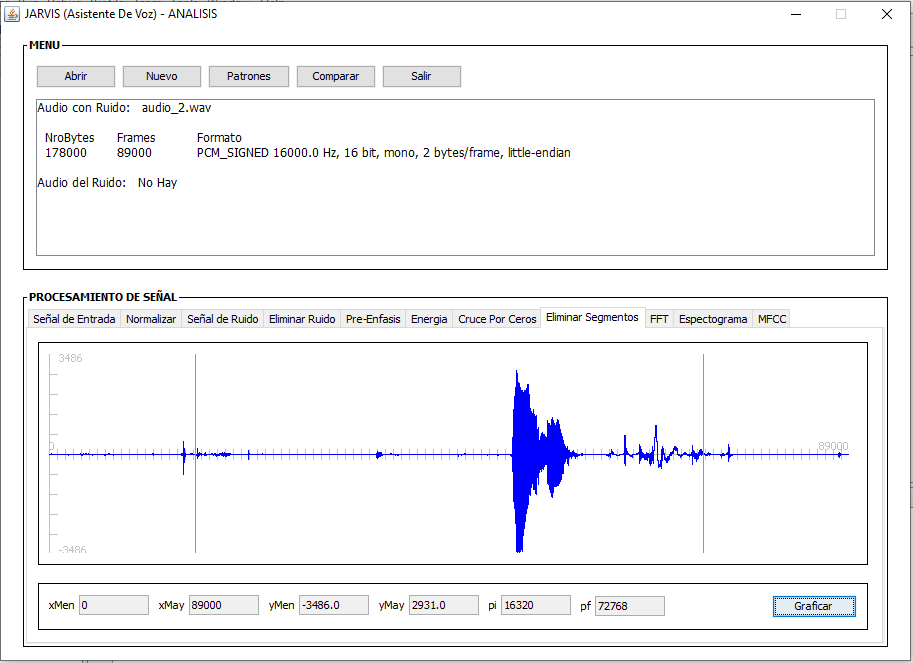
\includegraphics[width=0.65\textwidth]{Imagenes/Cap3/image074}
\end{center}
\begin{center}
\vskip -0.5cm
\caption{\small{Resultado del testeo para el \texttt{audio\_2.wav} por algoritmo de función de energía.}}
\label{fig:figura3.74}
{\small{Fuente: Elaboración propia}}
\end{center}
\end{figure}

\vskip -1.0cm

\begin{figure}[H]
\begin{center}
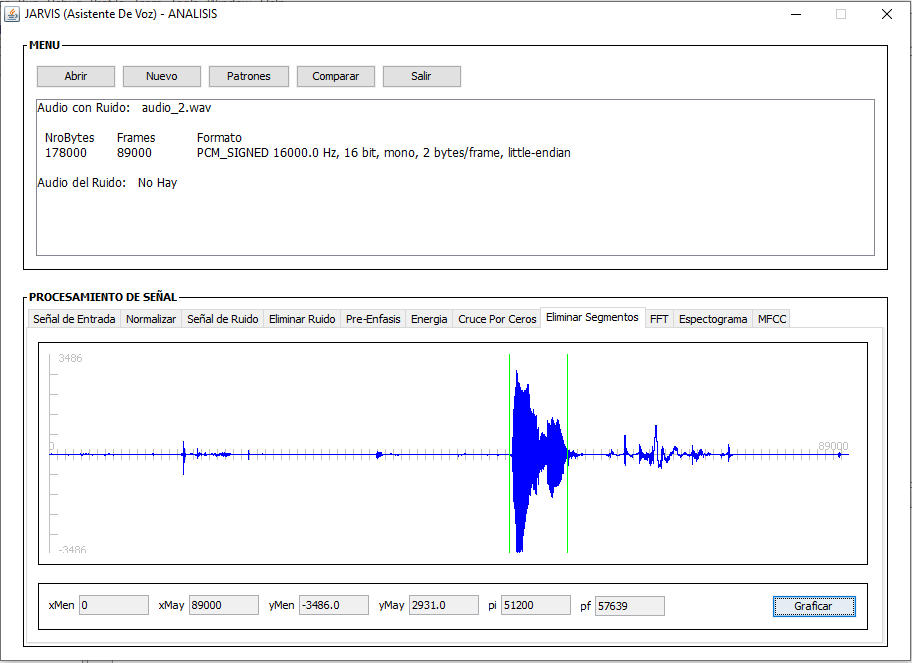
\includegraphics[width=0.65\textwidth]{Imagenes/Cap3/image075}
\end{center}
\begin{center}
\vskip -0.5cm
\caption{\small{Resultado del testeo para el \texttt{audio\_2.wav} por algoritmo de Rabiner \& Sambur tipo 1.}}
\label{fig:figura3.75}
{\small{Fuente: Elaboración propia}}
\end{center}
\end{figure}

\vskip -1.0cm

\begin{figure}[H]
\begin{center}
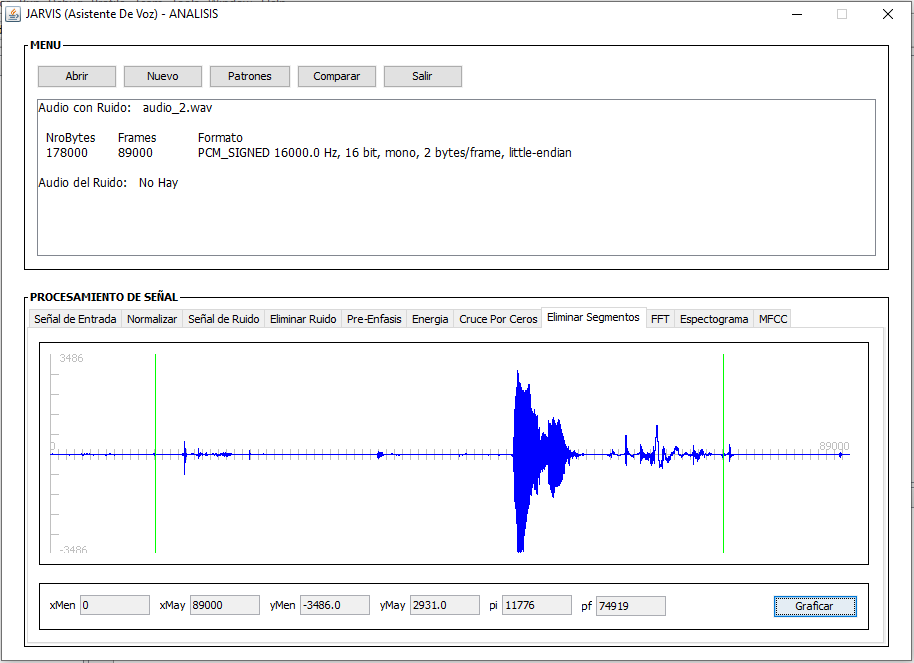
\includegraphics[width=0.65\textwidth]{Imagenes/Cap3/image076}
\end{center}
\begin{center}
\vskip -0.5cm
\caption{\small{Resultado del testeo para el \texttt{audio\_2.wav} por algoritmo de Rabiner \& Sambur tipo 2.}}
\label{fig:figura3.76}
{\small{Fuente: Elaboración propia}}
\end{center}
\end{figure}

De las Figuras \ref{fig:figura3.74}, \ref{fig:figura3.75} y \ref{fig:figura3.76} vemos que el algoritmo de Rabiner \& Sambur Tipo 1 recortó a la señal de voz mejor con respecto a los otros algoritmos, por lo tanto, se escogerá a este algoritmo para la etapa de Detección de Inicio y Fin de la Señal de Voz.

\subsection{Hallar el algoritmo para la eliminación de ruido aditivo}
Ahora pasaremos ah escoger el mejor algoritmo para la etapa de \textit{Eliminación de Ruido}, teniendo como configuración del algoritmo de reconocimiento de voz para el sistema: \\
- Algoritmo LMS\\
\hspace*{1cm} M = 128 ; \qquad $\mu$ = 0.02 y 0.002\\
- Algoritmo NLMS \\
\hspace*{1cm} M = 128 ; \qquad $\beta$ = 0.25, 0.025 y 0.0025 ; \qquad c = 0.0001
\vskip 0.5cm
Estas pruebas se realizaron con un micrófono primario ubicado a 2 metros de la fuente de ruido (en este caso fue la melodía de un celular) y un segundo micrófono ubicado a 50 cm de la fuente de ruido. Los micrófonos que se usaron fueron las de dos laptops y la palabra que se pronunció fue \textit{uno}, la grabación se realizó con una frecuencia de muestreo de 16000 Hz, canal mono, 16 bits de cuantificación y la codificación Little Endian.
\vskip 0.5cm
En la Figura \ref{fig:figura3.77} se muestra la señal de voz contaminada por el ruido capturada por el primer micrófono y en la Figura \ref{fig:figura3.78} se muestra la señal producida por la fuente de ruido capturada por el segundo micrófono.

\begin{figure}[H]
\begin{center}
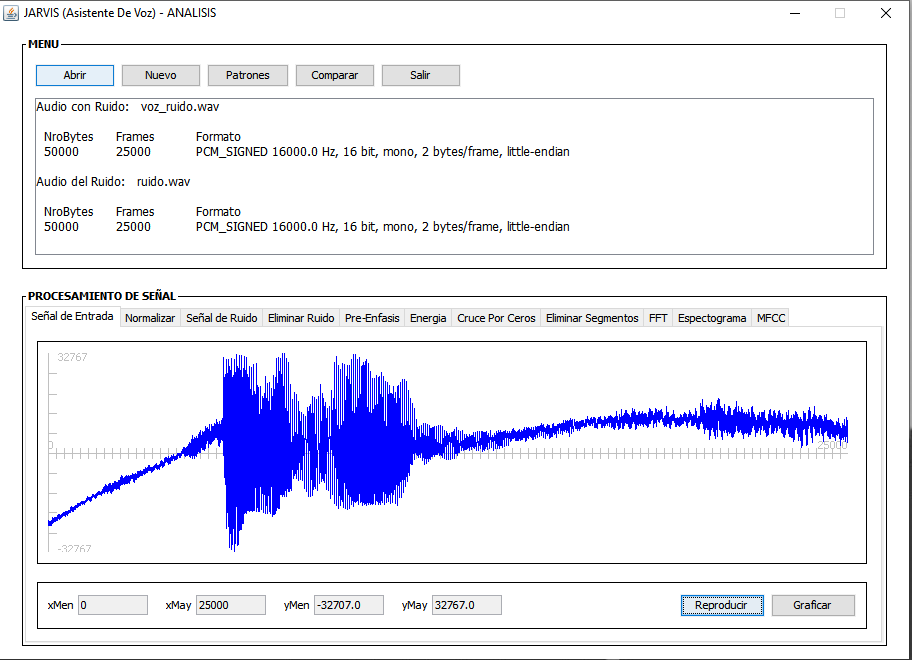
\includegraphics[width=0.65\textwidth]{Imagenes/Cap3/image077}
\end{center}
\begin{center}
\vskip -0.5cm
\caption{\small{Grafica de la señal de voz contaminada \texttt{voz\_ruido.wav}.}}
\label{fig:figura3.77}
{\small{Fuente: Elaboración propia}}
\end{center}
\end{figure}

\vskip -1.0cm

\begin{figure}[H]
\begin{center}
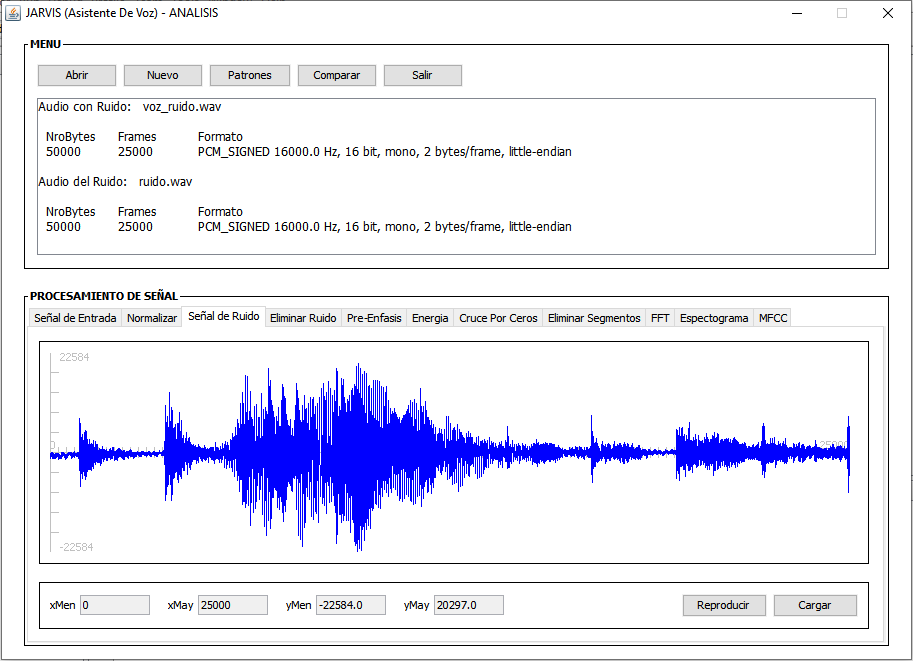
\includegraphics[width=0.65\textwidth]{Imagenes/Cap3/image078}
\end{center}
\begin{center}
\vskip -0.5cm
\caption{\small{Grafica de la señal de ruido \texttt{ruido.wav}.}}
\label{fig:figura3.78}
{\small{Fuente: Elaboración propia}}
\end{center}
\end{figure}

\begin{figure}[H]
\begin{center}
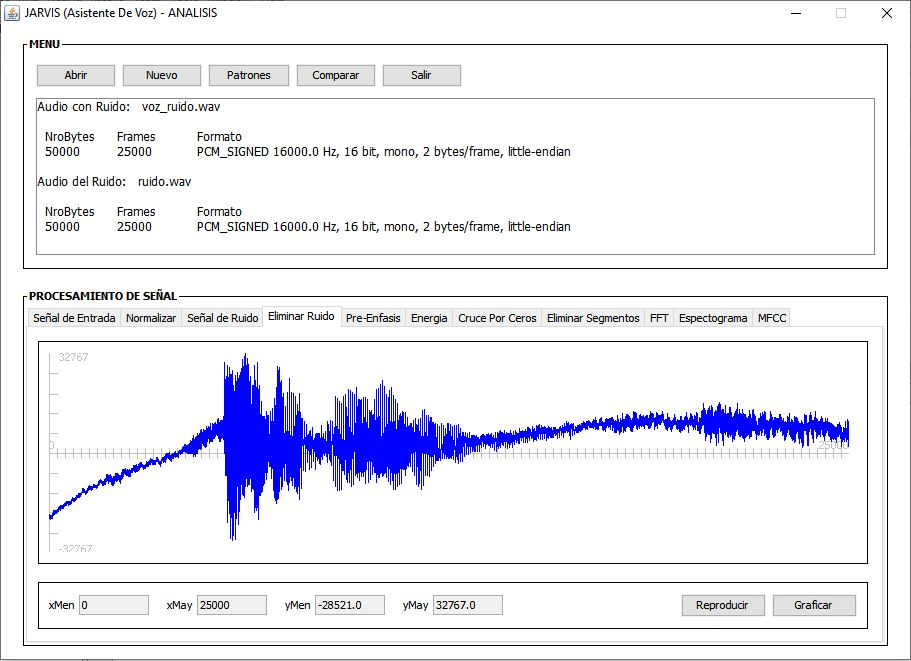
\includegraphics[width=0.65\textwidth]{Imagenes/Cap3/image080}
\end{center}
\begin{center}
\vskip -0.5cm
\caption{\small{Grafica de la señal después de aplicar LMS con $\mu$ =0.002.}}
\label{fig:figura3.80}
{\small{Fuente: Elaboración propia}}
\end{center}
\end{figure}

\vskip -1.0cm

\begin{figure}[H]
\begin{center}
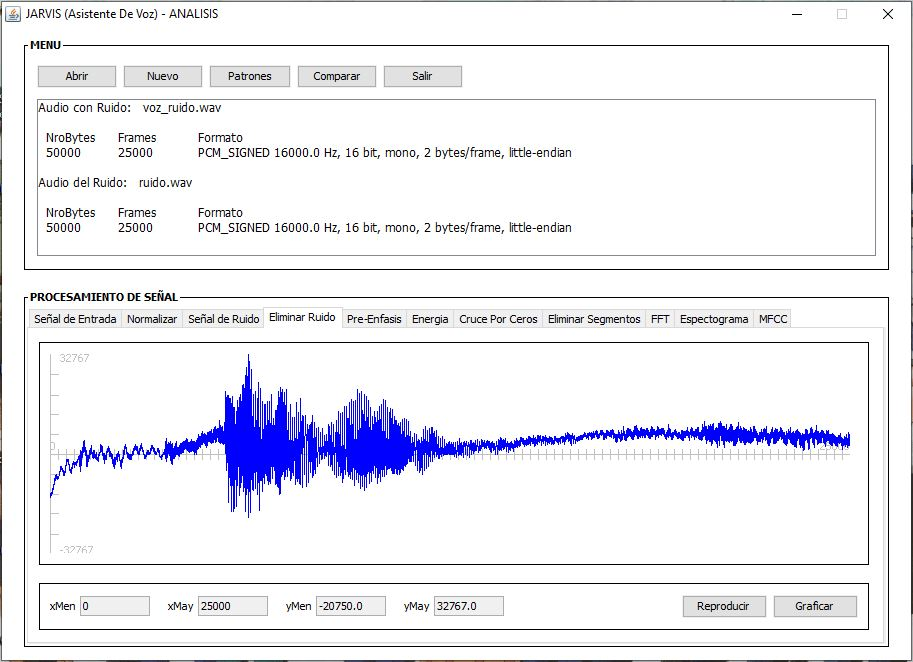
\includegraphics[width=0.65\textwidth]{Imagenes/Cap3/image083}
\end{center}
\begin{center}
\vskip -0.5cm
\caption{\small{Grafica de la señal después de aplicar NLMS con $\beta$ =0.0025.}}
\label{fig:figura3.83}
{\small{Fuente: Elaboración propia}}
\end{center}
\end{figure}

Las Figuras \ref{fig:figura3.80} y \ref{fig:figura3.83} se muestran los mejores resultados para cada algoritmo de esta prueba, podemos concluir que el mejor resultado para la eliminación de ruido lo obtuvo el NLMS con $\beta = 0.0025$, observamos que el ruido tiene una amplitud baja con respecto a la de la voz, por lo que resultará un mejor caso para la etapa de \textit{Detección de Inicio y Fin de la Señal de Voz}.

\begin{figure}[H]
\captionsetup{justification=centering}
\begin{center}
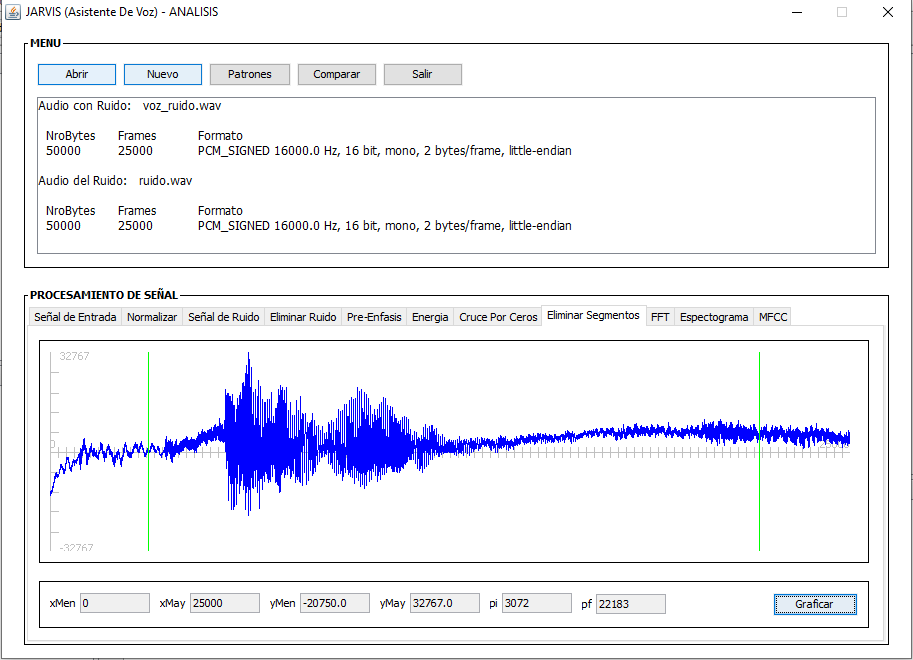
\includegraphics[width=0.65\textwidth]{Imagenes/Cap3/image084}
\end{center}
\begin{center}
\vskip -0.5cm
\caption{\small{Grafica de la señal para NLMS con \\ $\beta$=0.0025 y Rabiner \& Sambur Tipo 1 con T = 128.}}
\label{fig:figura3.84}
{\small{Fuente: Elaboración propia}}
\end{center}
\end{figure}

\vskip -1.0cm
Como vemos en la Figura \ref{fig:figura3.84} la señal no fue recortada perfectamente, el punto de fin de corte está muy lejos del final de la palabra esto se debe a que el sonido de la fuente de ruido tuvo mucho volumen pasando el rango de los 81 dBC que es el valor máximo para que funcione correctamente el algoritmo. Finalmente, podemos concluir de esta etapa de Testeo del Sistema que la configuración que tendrá el algoritmo de reconocimiento de voz para el sistema, es el siguiente:

\newpage
\begin{enumerate}

\item[•]Etapa de Eliminación de Ruido: 
\par
\hspace*{1cm} - Algoritmo NLMS \\
\hspace*{2cm} M = 128 ; \qquad $\beta$ = 0.0025 ; \qquad c = 0.0001

\item[•]Etapa de Detección de Inicio y Fin de la Señal de Voz: 
\par
\hspace*{1cm} - Algoritmo Rabinner \& Sambur Tipo 1 \\
\hspace*{2cm} T = 128

\item[•]Etapa de Entrenamiento: 
\par
\hspace*{1cm} - Filtro Preénfasis \\
\hspace*{2cm} $\alpha$ = 0.95 \\
\hspace*{1cm} - Segmentación por Hamming \\
\hspace*{2cm} V = 28 ; \qquad S = 18 \\
\hspace*{1cm} - Algoritmo MFCC \\
\hspace*{2cm} BC = 24 ; \qquad M = 15

\item[•]Etapa de Reconocimiento: 
\par
\hspace*{1cm} - Algoritmo DTW Simétrico \\
\hspace*{2cm} P = 1/2 ; \qquad R = 40 ; \qquad D = Error Cuadrático Medio \\

\end{enumerate}

\section{Fase 4. Mantenimiento del sistema}
Lo que haremos en esta etapa será implementar la configuración (funciones y parámetros óptimos) del algoritmo de reconocimiento de voz obtenida en la etapa de Testeo del Sistema, en la aplicación para el dispositivo móvil, además añadiremos a este el algoritmo el módulo de la toma de decisión, para luego poder probar nuestro sistema en un ambiente real.
\vskip 0.5cm
En la Figura \ref{fig:figura3.85} se muestra el código fuente del algoritmo para obtener el patrón característico (coeficientes MFCC) de una señal, usado en la etapa de entrenamiento.
\begin{figure}[H]
\captionsetup{justification=centering}
\begin{center}
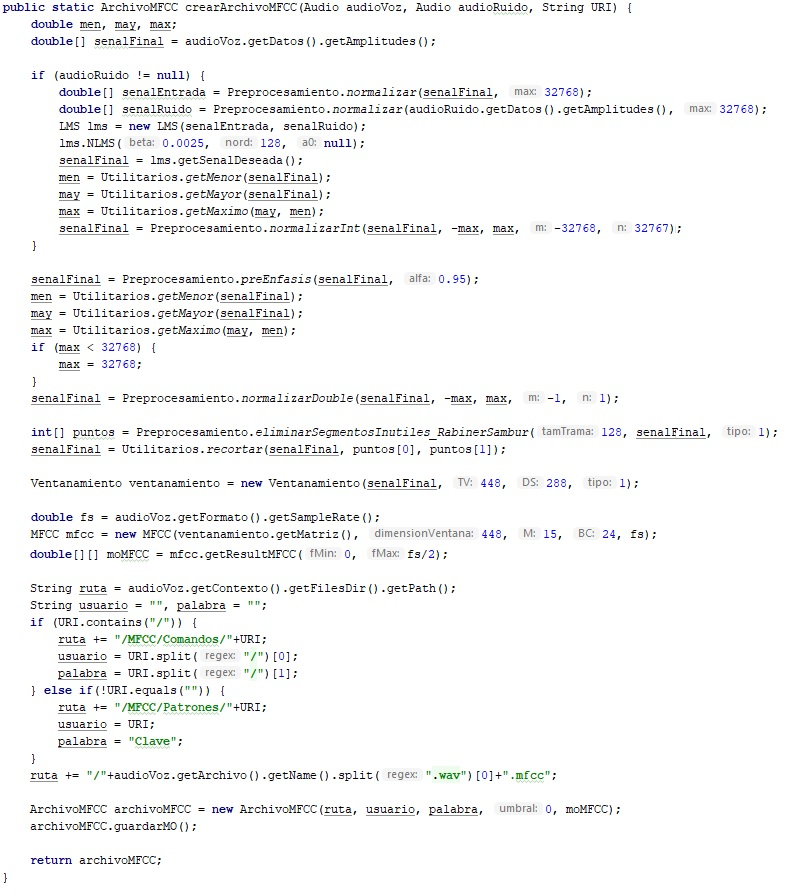
\includegraphics[width=0.85\textwidth]{Imagenes/Cap3/image085}
\end{center}
\begin{center}
\vskip -0.5cm
\caption{\small{Código fuente del algoritmo de reconocimiento de voz para la etapa de entrenamiento.}}
\label{fig:figura3.85}
{\small{Fuente: Elaboración propia}}
\end{center}
\end{figure}
\newpage
En la Figura \ref{fig:figura3.86} se muestra el código fuente del algoritmo para obtener el patron más parecido (menor medida de distancia) para una señal, usado en la etapa de reconocimiento.
\begin{figure}[H]
\captionsetup{justification=centering}
\begin{center}
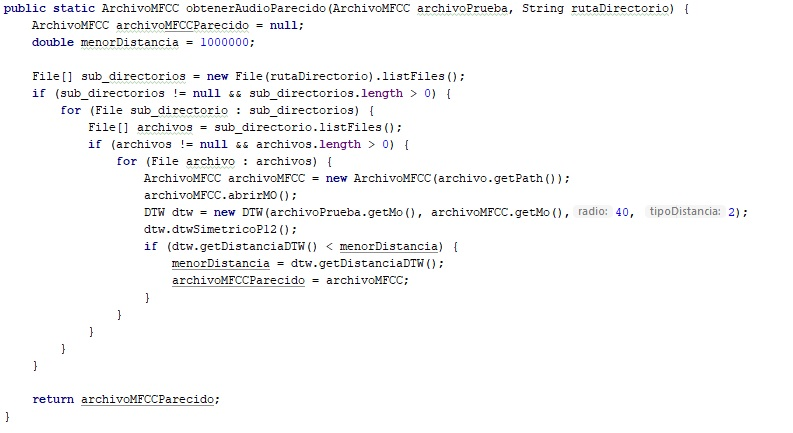
\includegraphics[width=0.85\textwidth]{Imagenes/Cap3/image086}
\end{center}
\begin{center}
\vskip -0.5cm
\caption{\small{Código fuente del algoritmo de reconocimiento de voz para la etapa de reconocimiento.}}
\label{fig:figura3.86}
{\small{Fuente: Elaboración propia}}
\end{center}
\end{figure}

En la Figura \ref{fig:figura3.87} se muestra el código fuente del algoritmo para obtener la respuesta del sistema (identificación correcta, no identificación y falsa identificación) ante la comparación de dos señales de voz, usado en la etapa de toma de desición.
\begin{figure}[H]
\captionsetup{justification=centering}
\begin{center}
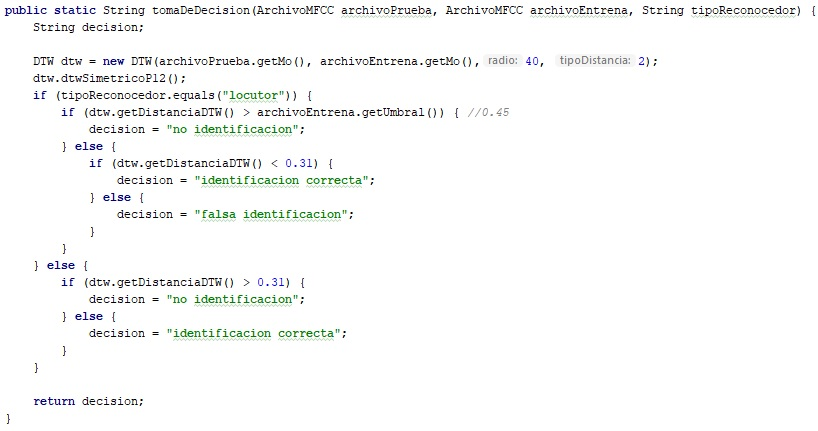
\includegraphics[width=0.85\textwidth]{Imagenes/Cap3/image087}
\end{center}
\begin{center}
\vskip -0.5cm
\caption{\small{Código fuente del algoritmo de reconocimiento de voz para la etapa de toma de decisión.}}
\label{fig:figura3.87}
{\small{Fuente: Elaboración propia}}
\end{center}
\end{figure}

En las Figuras \ref{fig:figura3.88} y \ref{fig:figura3.89} se muestran las funciones para obtener los umbrales para la toma de desición del sistema definido por las Ecuaciones \eqref{eq:ecuacion105} y \eqref{eq:ecuacion106}.
\begin{figure}[H]
\captionsetup{justification=centering}
\begin{center}
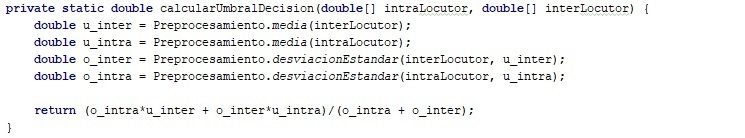
\includegraphics[width=0.85\textwidth]{Imagenes/Cap3/image088}
\end{center}
\begin{center}
\vskip -0.5cm
\caption{\small{Código fuente de la función de cálculo del umbral de decisión.}}
\label{fig:figura3.88}
{\small{Fuente: Elaboración propia}}
\end{center}
\end{figure}

\begin{figure}[H]
\captionsetup{justification=centering}
\begin{center}
\includegraphics[width=0.85\textwidth]{Imagenes/Cap3/image089}
\end{center}
\begin{center}
\vskip -0.5cm
\caption{\small{Código fuente para la obtención de los umbrales de decisión para cada patrón de entrenamiento.}}
\label{fig:figura3.89}
{\small{Fuente: Elaboración propia}}
\end{center}
\end{figure}
